\documentclass[%
        paper=a4,
	% BCOR=10mm, % Binding CORrection
	twoside,			% two sided printing
        %cleardoublepage=empty,         % empty backsides for two sided printing
        twocolumn=false,
	titlepage,			% support for title environment
	numbers=noenddot,		% numbers (in headlines) without ending points
	chapterprefix=false,            % chapter names without prefix "Chapter"
	headsepline,			% line below header
	%footsepline,			% line above footer
	headings=normal,                % size of header is normal
	fontsize=11pt,			% fontsize in points
	pagesize=pdftex,		% define typearea for pdftex usage
        headheight=46.96317pt,          % value based on MyThOS logo
        parskip=off                     % or half*
]{scrbook}

% ------------------------------------------------------------------------------
% character encoding and fonts for the document
\usepackage[T1]{fontenc} % should be loaded before inputenc
\usepackage[utf8]{inputenc}	    % unicode, newer than utf8x
\usepackage{ae}
\usepackage{aecompl}
\usepackage[T1]{url}			% web adresses with t1 style
\urlstyle{tt}					% web adresses in tt-style
\usepackage[UKenglish]{babel}

% ------------------------------------------------------------------------------
% font setup
\usepackage{microtype}
\usepackage{ellipsis}			% corrects wrong spaces after dots
\usepackage{amsmath}
%\usepackage{amsfonts}
\usepackage{amssymb}
\usepackage{latexsym}
\usepackage{dsfont}

%% bera mit euler
\usepackage{bera,amssymb,eufrak}
\usepackage[euler-digits,euler-hat-accent]{eulervm}

\setlength{\parskip}{0.5em plus 1em minus 0.5em}
\clubpenalty 2000
\widowpenalty 2000
%\setlength{\tolerance}{2000}
\setlength{\emergencystretch}{20pt}   % kann man evtl. auf 20 erhöhen
%\setlength{\hfuzz}{1pt}
\setlength{\hfuzz}{10pt}

% ------------------------------------------------------------------------------
% pdf creation
\usepackage[%
  pdftitle={MyThOS Base Architecture ver.2},
  pdfsubject={Technical Report},
  pdfauthor={Robert Kuban, Randolf Rotta},
  pdfkeywords={MyThOS}, % comma separated
  pdftex,
  colorlinks=true,
  urlcolor=red,
  citecolor=red,
  linkcolor=red,
  bookmarks=true,
  breaklinks=true
]{hyperref}

% ------------------------------------------------------------------------------
% graphics
\usepackage[usenames,dvipsnames]{xcolor}
\usepackage{graphicx}
\usepackage{subfigure}
\usepackage{tikz}
\usetikzlibrary{calc,trees,positioning,arrows,chains,shapes.geometric,%
    decorations.pathreplacing,decorations.pathmorphing,shapes,%
    matrix,shapes.symbols}

% ------------------------------------------------------------------------------
% listings
\usepackage{listings}		% include listings
\newcommand{\code}{\lstinline}
\lstloadlanguages{C++}
\lstset{
  basicstyle=\ttfamily\footnotesize,
  keywordstyle=\bfseries,
  stringstyle=\textit,
  emphstyle=\textit,
  commentstyle=\textit,
  breaklines=true,
  breakatwhitespace=true,
  breakautoindent=true,
  morekeywords={},
  numbers=left,
  numberstyle=\tiny\color{black},
  stepnumber=1,
  numbersep=5pt,
  tabsize=2,
  showspaces=false,
  showstringspaces=false,
    xleftmargin=17pt, 			% left margin where linenumbers and frames do start
    framexleftmargin=17pt, 		% left margin of frame (which will be colored)
    framesep=0pt,
    belowcaptionskip=0pt,
    captionpos=b,
    framerule=1pt
}

\usepackage{scrhack}
\usepackage{float}
\floatstyle{plain}
\newfloat{listing}{tbhp}{myc}
\floatname{listing}{Listing}

% ------------------------------------------------------------------------------
% tables 
\usepackage{multirow}
%\usepackage{ragged2e}
\usepackage{tabularx}
\usepackage{longtable}
\usepackage{booktabs}   % toprule, midrule in Tabellen
\newcolumntype{Y}{>{\raggedright\arraybackslash}X}
\usepackage{caption}

\usepackage{collcell}
\newcolumntype{L}{>{\collectcell\lstinline}l<{\endcollectcell}}
\newcolumntype{R}{>{\collectcell\lstinline}r<{\endcollectcell}}

\usepackage{bytefield}

%------------------------------------------------------------------------------
\usepackage{xspace}
\newcommand{\mythos}{\textsc{MyThOS}\xspace}
\def\cc{{C\nolinebreak[4]\hspace{-.05em}\raisebox{.4ex}{\tiny\bf ++}}}

\usepackage[textsize=tiny]{todonotes}

\usepackage{enumerate}
\usepackage{epigraph}
\renewcommand{\epigraphsize}{\footnotesize}
\setlength{\epigraphwidth}{0.618\textwidth}


% ------------------------------------------------------------------------------
\title{MyThOS Base Architecture ver.2}
\author{Robert Kuban, Randolf Rotta}

\titlehead{
\begin{center}
  \noindent\rule{1.0\textwidth}{1pt}\\[1cm]
  
\includegraphics[scale=0.5]{MyThOS_Logo}\\[0.5cm]
  \sffamily
  \small
  \begin{tabularx}{\textwidth}{lX}
    Förderkennzeichen: & 01IH130003 \\
    Vorhabensbezeichnung: & MyThOS \\
    & Modulares Betriebssystem für Massiv Parallele Anwendungen
  \end{tabularx}\\[0.5cm]
  \noindent\rule{1.0\textwidth}{1pt}
\end{center}
%\vspace{1cm}
}


\usepackage{scrlayer-scrpage}
\setkomafont{pageheadfoot}{\sffamily\small}
\lohead{%
MyThOS Base Architecture ver.2\\%
\headmark%
}
\cohead{}
\rohead{
\includegraphics[height=1.5cm]{MyThOS_Logo}}
\pagestyle{scrheadings}

%\usepackage{showframe}

% ------------------------------------------------------------------------------
% layout
\usepackage{multicol}
\usepackage{marginnote}
\renewcommand*{\marginfont}{\footnotesize}
\typearea[current]{last}		% recalculate type area

\begin{document}
\frontmatter			% start numbering pages
\maketitle
\tableofcontents
\mainmatter
% ------------------------------------------------------------------------------
% content

\chapter{Preface}

\epigraph{The only way to avoid these traps is to encourage a software culture that knows that small is beautiful, that actively resists bloat and complexity: an engineering tradition that puts a high value on simple solutions, that looks for ways to break program systems up into small cooperating pieces}{Eric S. Raymond, The Art of UNIX Programming}


\section{Issues with Previous MyThOS Designs}

\begin{enumerate}[(1)]
\item The object capabilities were present as a translation table from user-visible logical identifiers to actual kernel-level pointers. However, these translations did not cooperate with the resource management. Hence, it was possible to delete kernel objects without cleaning up all dangling references. Deletion could overlap with concurrent method calls to the deleted object.
\item The object capabilities translated just to kernel objects and any access control was implemented by pointing to a more restricted interface. Combining all relevant access rights, for example readable, writeable, delegatable, referencable, and so on, leads to a combinatorial explosion of interface variants.
\item Each execution context (user thread) required a dedicated kernel stack that was used for the entry from system calls and interrupts. These stacks were mostly unused because the kernel's task scheduling had to switch to the hardware thread's main stack anyway. Allocating and mapping these kernel stacks into the kernel space increased the thread creation overhead. 
\item All kernel objects were placed into specific expandable logical address ranges in the kernel space. The implied dynamic kernel address space management introduced dependencies to physical memory allocators for the on-demand creation of page maps. This introduced non-deterministic overheads whenever the kernel space page maps had to be updated.
\item In order to improve the scalability of the kernel's internal memory allocators, private memory pools were used at each hardware thread. Because of the limited memory capacity, these pools had to allocate from a globally shared reserve anyway. The assignment of resources to these pools and the return to the global pool required complex policies, statistics, and algorithms. Nevertheless these strategies did not match the application's actual needs.
\item The implicitly allocated kernel-space objects had no user-visible address. Hence, there was no mechanism to clean up and recycle these resources on demand. Smart pointers with reference counting were used at some places but did not cooperate well with the translation of user capabilities to kernel objects. Especially, it was easy to create cyclic dependencies that would never get cleaned up. This could have been solved with a much more restrictive process-thread model, tying the kernel and supervisors to a quite limited policy.
\item The high-level stubs for system calls tried very hard to resemble a homogeneous symmetric remote method invocation model similar to, for example, JavaRMI. This made the actual implementation of kernel objects and services overly difficult because the generated kernel-side stubs either hid too much context information, for example the calling process and numeric object handles, or pre-processed the arguments more than actually needed by the kernel object. 
\item The generator for the high-level stubs increased dependencies on complex tools like the python-clang binding. Despite all the help from modern compilers, extracting interface definitions from the kernel's C++ code had a hard time to separate interface-relevant information from unrelated definitions. This polluted the user-space client stubs with arbitrary kernel-internal definitions. 
\item Like with the widely used locks for critical code sections, all synchronisation was in the responsibility of the users/callers of kernel objects and services like the address space management. However, often the caller side did not know the exact synchronisation requirements , or the correct core, that was supposed to process the requests. Therefore, some synchronisation was overly pessimistic while some was insufficient and led to race conditions.
\item The kernel-level asynchronous communication between hardware threads was unbounded based on the on-demand allocation of message buffers. This introduces hidden overheads for the allocation and deallocation of messages. The missing flow control allowed misbehaving code to use up all kernel memory. Likewise, the asynchronous inter-process communication service allowed misbehaving applications to deplete all kernel memory.
\item The kernel operated without masking the interrupts. All data structures based on atomic operations required careful design in order to avoid deadlocks created by interrupts at intermediate steps---especially when interrupt handlers might access the same data structures. Hence, complex wait-free data structures had to be used instead of simpler lock-free and obstruction-free variants. In consequence, interrupts had to be disabled at quite some places anyway.
\end{enumerate}


\section{Many-Core Challenges with Existing (Micro-)Kernel Architectures}

\begin{enumerate}[(a)]
\item Synchronous IPC and synchronous system calls: Long running operations such as resource cleanup, e.g.\ a capability revoke, block the calling thread. In order to offload such work to another thread, a complex combination of asynchronous notifications and user-level communication via shared memory is needed.
\item Big Kernel Lock versus fine grained locking versus replication: The Big Kernel Lock is a kernel monitor, which ensures that at any point of time at most one thread operates on the kernel's data. It simply sequentialises all system calls and interrupt handling and enables the use of very efficient low-overhead data structures and algorithms. However, the parallel scalability is obviously limited. Fine grained locking and nonblocking data structures reduce the serial fraction but increase the management overhead (space for locks, frequent acquire\&release operations) considerably. Multikernel and Clustered Multikernel exploit the big kernel lock's efficiency locally and use a higher message-based coordination layer globally. The scalability depends on the throughput of the replication mechanism.
\item Read-Copy-Update: This mechanism provides a quite restricted form of transactional memory and is well suited to increase the throughput of write operations on queues, lists, and trees. Is not a general purpose synchronisation mechanism and, hence for example, most critical sections in Linux still have to rely on (spin-) locks for mutual exclusion. The delayed visibility of the newest copy and delayed deletion of outdated copies implies the need for on-demand memory allocation for new copies. This introduces a dependency to a shared memory pool for these copies.
\item Frequent address space switching: 
\item Not all microkernels are as small and simple as desirable for many-core processors: Kernel-level on-demand memory allocation and deallocation add considerable complexity. The separation between core kernel components and platform- and application-specific extensions is not always clear, which hampers the extensibility.
\item Licensing: While some kernels are available under BSD-alike licenses, we repeatedly found crucial code under GPL license, for example in code generators for stubs and data structure access.  
\end{enumerate}


\section{Key Aspects of the Presented Design}

\begin{itemize}
\item No on-demand memory allocation and deallocation inside the kernel: objects are created only through user requests (system calls) and the user supplies the needed memory pool.
\item No logical/virtual memory in the kernel space: after booting, the kernel's logical to physical address translation tables are not extended, which removes the need for on-demand page maps. The kernel operates inside a 4GiB direct-mapped address range, which removes the need to differentiate between physical and logical addresses and enables compact 32bit pointers.
\item No direct access to user-space memory: the user tells the kernel which frames will be used for sharing between kernel and user space. The kernel accesses the physical frames directly, which removes all in-kernel page faults and dependency on the user-space address translation.
\item No interrupts during usual kernel-mode execution: Just the kernel's task scheduler contains a preemption point to check for pending interrupts. All kernel tasks are very short running or decompose into multiple tasks and can be implemented more efficiently when interrupts do not need to be feared.  
\item Unified smart pointer and weak reference mechanism, includes precise tracking of resource inheritance. This is used for long-term storage of references and enables to inform all affected reference holders and tear down all contained sub-resources.
\item Unified translation from user handles to kernel objects: Separate translation table implementations for the various types of user-visible kernel objects are no longer needed. Instead the user space references any type of kernel objects through capability pointers and these are translated into kernel objects and access rights through per-process capability spaces. The capability spaces are the user's entry point to the kernel's unified resource management and prevent premature deletion of kernel objects.
\item Simplified software layers: The synchronisation mechanisms do no longer need to differentiate between purely local synchronisation and remote communication. It is no longer necessary trying to choose a appropriate memory allocators in various places all over the kernel, which often fails because information about future sharing of the allocated memory is not available. Now, only factories for kernel objects allocate memory and are passed appropriate memory allocators by the caller.
\item No implicit sharing of kernel objects between processes, user threads, and hardware threads. Through the explicit allocation of kernel objects and user-driven partitioning of the physical memory pool, the applications have full control over all aspects of sharing.  
\item Non-blocking synchronisation in shared kernel objects: A delegation mechanism based on small task objects unifies various types of synchronisation monitors and provides lightweight non-blocking mutual exclusion. The monitors automate the flow control such that no on-demand allocation of message/task buffers is necessary.
\item Unified event-style task execution model: System calls, interrupt epilogues, delegated critical sections, asynchronous method calls, and the return to user-mode execution are expressed through small tasks and are scheduled by a lightweight scheduler on each hardware thread.
\item The kernel code does not hide that all addresses are in the direct mapped part of the kernel space. Physical addresses can be easily accessed by adding the direct mapping base address and physical addresses can be obtained from kernel addresses by subtraction.
\end{itemize}

\section{Relation to seL4}

It is undeniable that the design of \mythos as presented in this document borrowed many clever ideas from the seL4 design and implementation. We are very thankful for the inspiring papers and presentations of Gernot Heiser et al. and the decades of collective experience on which this work could build upon. Many projects, for instance also the Barrelfish multikernel, learned a lot from seL4, which helped to speed up development and allow to focus on specific key aspects. Despite the many similarities, \mythos features a few interesting differences, which we hope to be very useful for the targeted HPC application scenarios:  

\begin{itemize}
\item seL4's prefix serialisation of the capability derivation tree is used in \mythos for the prefix serialisation of the resource inheritance tree. We analysed the inheritance rules and successfully separated the tree management from any type-specific knowledge about kernel objects. Kernel objects implement a simple C++ interface in order to take part in the kernel's resource management.
\item seL4's compact storage of in-kernel pointers was applied to the resource inheritance tree in order to achieve a very compact representation even on 64-bit processors. By coincidence, the 64-bit variant does not consume more memory than seL4's 32-bit variant. 
\item \mythos replaces seL4's widespread use of switch-case type dispatches by C++ virtual methods of the kernel object interface. This enables the easy introduction of new kernel objects for specific use cases and hardware-specific device support. Whether the virtual method dispatch is faster than seL4's long chains of conditional branches has to be seen. Of course, such vtable-based dispatches complicate formal verification very much. 
\item The Untyped Memory objects in seL4 use a simple watermark scheme. This simplifies verification but leaves significant (internal) fragmentation when large kernel objects like page maps require a specific alignment. The \mythos design allows for the use of in-place free lists and similar heap structures inside the Untyped Memory objects. It still needs to be evaluated which variant balances overhead and compactness well enough.
\item Through the monitors and scheduling contexts, the \mythos kernel has an understanding of the processor's distributed topology. This makes it possible to assign kernel services and application threads to dedicated cores.
\item \mythos has no big kernel lock and allows concurrency inside the kernel. Lightweight non-blocking synchronisation and delegation are used to protect shared kernel objects. However, the decision to share kernel objects between hardware threads is a pure application choice. The kernel can be operated like a multikernel or a clustered multikernel. Of course, respective implementation variants should be selected to skip superfluous synchronisation.
\item Based on the scheduling contexts, the kernel's inter-process communication supports deferred synchronous communication between different hardware threads. Most L4-based kernels support just asynchronous notifications based on inter-process interrupts between hardware threads.
\item \mythos separates the sender-side communication portal from the user thread. This allows applications to set up multiple portals per thread in order to enable multiple overlapping deferred synchronous system calls and IPC messages. We hope that this simplifies the implementation of user-level asynchronous programming frameworks.
\item The resource management around the inheritance tree, kernel objects, and factory objects is designed to simplify the introduction of new kernel objects with minimal impact on the existing base kernel.
\end{itemize}


\section{Current Limitations}

\begin{itemize}
\item Capability transfers are not implemented. Instead the supervisor should manipulate the capabilities directly in the Capability Maps of supervised applications.
\end{itemize}

\chapter{Architecture Overview}
\label{chapter:arch-overview}

\epigraph{Unix's syscalls all are synchronous. That makes them a bad target for a microkernel, and the primary reason why Mach and Minix are so bad - they want to emulate Unix on top of a microkernel. Don't do that.

If you want to make a good microkernel, choose a different syscall paradigm. Syscalls of a message based system must be asynchronous (e.g. asynchronous IO), and event-driven (you get events as answers to various questions, the events are in the order of completion, not in the order of requests). You can map Unix calls on top of this on the user side, but it won't necessarily perform well.}{Bernd Paysan, alt.os.multics, 2003.}

\noindent
This chapter discusses the global architecture and gives an overview
about the basic abstractions and dynamics of the system.
Subsequent chapters focus in more detail on individual subsystems.

The following sections follow the 4+1 view model of Kruchten~\cite{kruchten19954+}.
The first section summarises the requirements as Application View. 
Section~\ref{sec:global-logical-view} describes the logical view, which consist of common services, mechanisms, and design elements that fulfill the functional requirements.
The physical view in Section~\ref{sec:global-physical-view} discusses the deployment with respect to the placement and replication of components onto processors and hardware threads as well as the basic memory layout.
Subsection~\ref{sec:global-dynamical-view} discusses the dynamical view, which focuses on interactions inside the kernel, between applications and kernel, and between applications as well as the life-cycle management of components and the necessary scheduling.
Finally, the development view in Section~\ref{sec:global-development-view} describes implementation aspects, for example, the files and folders structure and the configuration management via code modules.

%%%%%%%%%%%%%%%%%%%%%%%%%%%%%%%%%%%%%%%%%%%%%%%%%%%%%%%%%%%%%%%%%%%%%%
\section{Application View}
\label{sec:global-application-view}

The target application domain of MyThOS is dynamic and elastic high-throughput parallel 
computing applications on many-core processors. 
%
For example, complex multi-physics simulation codes exhibit multiple coupled applications operating in turns and in parallel on shared data. \emph{Invasive computing}~\cite{InvasiveComputing,octopos} tackles the difficult load balancing by trading cores dynamically between the individual applications.
%
Similarly, new applications in big data, deep learning, and the internet of things raise the need for \emph{elastic} compute clouds~\cite{Rhoden:2011:IPE:2038916.2038941}. In addition to the dynamic assignment of cores to compute tasks, these scenarios require effective isolation and supervised communication between third-party compute codes.

The requirements from the application's viewpoint divide into three general
types of user-space activities: actual applications that perform computations,
supervisors that globally coordinate between the applications, and basic system
services that provide a shared infrastructure.
The supervisors require mechanisms to exert control over applications such as
assigning and revoking physical memory, storage in general, compute cores, and communication channels.
This includes the ability to preempt and migrate application threads as well as 
to intercept protection violations and similar events. In this way, 
policies such as the mapping of application threads to physical cores and invasive computing~\cite{InvasiveComputing} can be implemented.
Beyond this, the three types share requirements with respect to the management
of threads, address spaces, shared memory, and communication.

Application threads provide logical control flows that are scheduled for 
execution by the operating system and operate in an application-specific 
environment.
Interfaces are needed to create/delete and 
suspend/wakeup application threads.
The thread's execution environment is composed of a logical address space, 
thread-specific data (stack, basic communication buffers, thread-local data) 
inside this address space and access rights to system services and 
communication channels.    
Hence, an interface is needed to map actual memory into these address spaces and configure the processor's support for thread-local data.
On many-core processors, an additional core-local storage relative to 
physical hardware threads seems useful.

Basic communication support by the OS kernel is needed for inter-process communication (IPC) between application, supervisors, and system services, e.g., to communicate requests and set up high-level communication.
If system services are partially implemented by kernel objects instead of user-space threads, a uniform interface is needed to hide the implementation-specific differences.  
High-volume data transfers are usually facilitated via shared memory, which requires means to setup shared memory across address spaces.
In this context, asynchronous and optionally preemptive notification mechanisms
are useful in order to avoid busy polling on shared message buffers.
The actual communication between application threads is up to the application's parallel programming runtime. 


%%%%%%%%%%%%%%%%%%%%%%%%%%%%%%%%%%%%%%%%%%%%%%%%%%%%%%%%%%%%%%%%%%%%%%
\section{Logical View}
\label{sec:global-logical-view}

This section describes the logical view, which consist of common services, mechanisms, and design elements that fulfill the functional requirements of the system.

From the application's point of view, abstractions for communication with the operating system services, for communication with other applications, and for the management of their execution environment are needed. These abstractions define the overall system's style and versality.
For example, Unix-based systems expose a large number of kernel functions via the system call interface. Where a reference to a specific instance, for example a file, is needed, a numeric handle, for example a file descriptor, is passed via the call arguments and the kernel function looks up the instance in a type- and process-specific table.
Other designs focus directly on these instances and let the application communicate with them via a small set of system calls, see for example~\cite{Liedtke1996}. This style is closer to method invocations on kernel objects. A major advantage is, that the management of instances can be unified while giving the application/user more explicit control.

\subsection{Vertical Layers and Object Types}
\label{sec:vert-layer}
% problem statement
Different styles of interaction between objects can be found inside the kernel. This is caused by the differentiation between purely local actions that do not leave their hardware thread, communication mechanisms that coordinate the kernel's activities across hardware threads, and the communication between user-mode applications and kernel via system calls and invocation messages.

This section introduces vertical layers of the software architecture in order to simplify the later discussion of the respective interaction styles. The interaction styles also constrain the object model in order to lead to interoperable interfaces. A short summary of the layers and object models in shown in Figure~\ref{fig:layers}.

% \begin{table}
% \caption{Vertical layers and object types.}
% \label{tab:layers}
% \begin{tabularx}{\textwidth}{l|lYY}
% \toprule
% layer & object type & object interface & layer implements \\ 
% \midrule 
% synchronous & C++ obj. & C++ method calls,\newline immediate execution & hardware abstractions, runtime for async. layer\\ 
% asynchronous & async. obj. & Tasklet passing,\newline deferred execution & shared/distributed kernel-level services \\ 
% managed & kernel obj. & async. invoke handler, capability as weak ref. & system calls and comm. for applications \\
% application & cap. ptr. & capability invocation & applications, supervisors, user-level services \\
% \bottomrule
% \end{tabularx}
% \end{table}

\begin{figure}
  \centering
  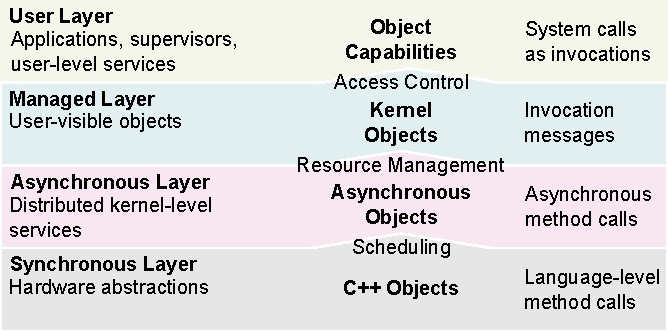
\includegraphics[scale=1]{slides/figures/layers.pdf}
  \caption{Vertical layers and object types.}
  \label{fig:layers}
\end{figure}

\begin{description}

\item[Synchronous Layer:] This is the lowest, most basic layer of the architecture. Ordinary \emph{C++ objects} are used to implement fundamental data structures and basic hardware abstraction components. These objects are used via the ordinary C++ method and function calls and their implementation is executed immediately in the current logical control flow.

This layer is responsible to provide the runtime environment that is needed by the asynchronous layer. This includes the scheduling of asynchronous activities across hardware threads and mechanisms for concurrency and locality control. \emph{Tasklet} objects provide the abstraction for asynchronous activities and \emph{monitor} objects implement asynchronous synchronisation policies such as mutual exclusion.

\item[Asynchronous Layer:] On top of the runtime environment from the synchronous layer, this layer hosts \emph{asynchronous objects} that provide communication via asynchronous method calls. In contrast to arbitrary C++ object methods, the asynchronous methods consume a Tasklet as small state buffer and a reference to an asynchronous response handler object. The actual implementation of the called method can be executed at a later time and also on a different hardware thread. The call returns by calling a respective asynchronous response method, passing along the Tasklet. 

This layer implements shared kernel infrastructure and is not directly visible to the user. Examples are the \emph{resource inheritance tree} and supporting asynchronous objects for the implementation of kernel objects.

\item[Managed Layer:]
\marginnote{See also~\ref{sec:capability-impl}}
This layer manages the resources and life cycle of \emph{kernel objects} through \emph{capabilities} as an unified smart pointer mechanism. The capabilities track the resource inheritance beginning from memory ranges over kernel objects allocated in this memory to derived weak references that point to the same kernel object. In cooperation with the memory management this inheritance enables the clean deallocation of kernel objects and recycling of the respective memory. 
Alongside the basic state information that is used by the kernel's resource management, the capabilities include generic and type-specific access rights. These are used by the system call interface to restrict the user's capability invocations. Such invocations are forwarded as asynchronous method call's to the \emph{invoke()} method of the targeted kernel object.

This layer contains all user-visible and call-able system services, which are introduced in Section~\ref{sec:kernel-objects}. A small set of system calls allows to push capability invocations from the application to the kernel objects.

\item[Application Layer:] Applications, supervisors, and other system services live in the application layer. Application threads interact with \emph{kernel objects} via \emph{capability pointers}, which are logical indexes into the thread's capability space. Communication on the application layer is possible via shared memory in the logical address spaces and via inter-process communication (IPC) services of the kernel. Libraries can introduce various middleware layers for higher-level parallel abstractions.
\end{description}

\subsection{Core Abstractions: Kernel Objects}
\label{sec:kernel-objects}

\begin{figure}
  \centering
  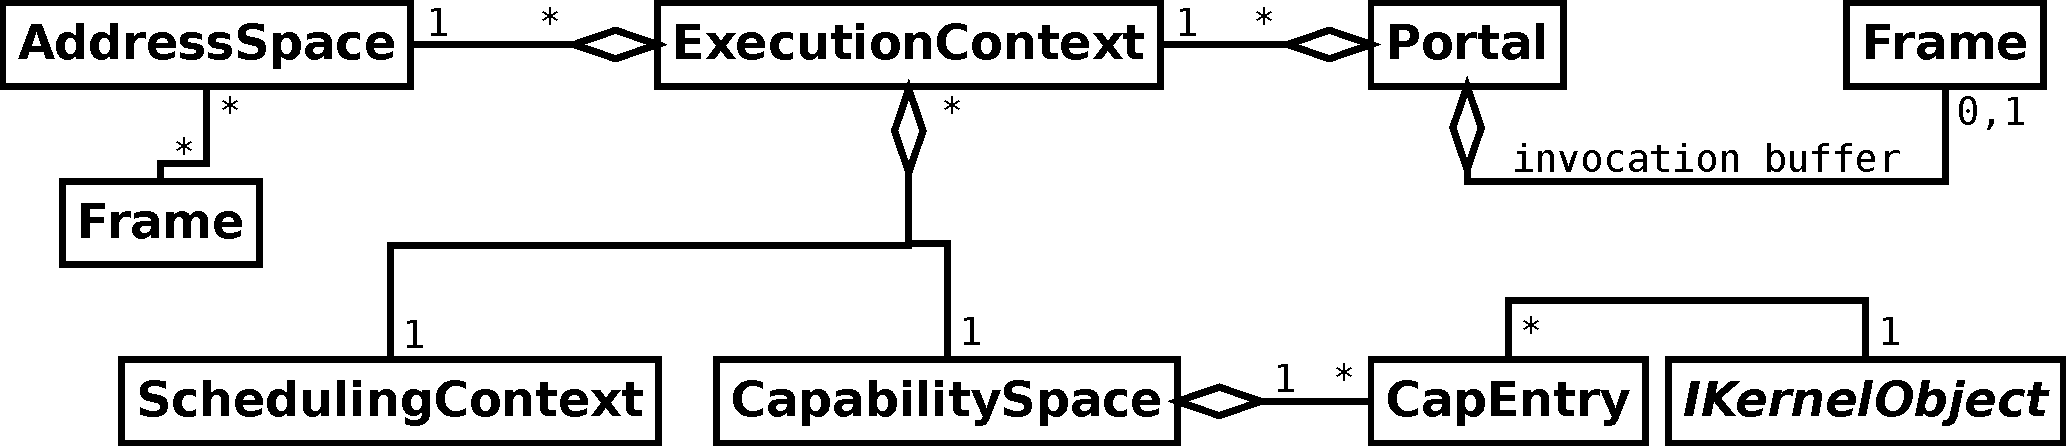
\includegraphics[scale=0.25]{fig/kernel-objects-logical.pdf}
  \caption{Interaction between the basic kernel objects.}
  \label{fig:kernel-objects-logical}
\end{figure}

\emph{Kernel objects} are the smallest components with a managed life cycle. Figure~\ref{fig:kernel-objects-logical} shows a class diagram of the interactions between the core kernel objects. 

\begin{description}
\item[Address Space:]
\marginnote{See also~\ref{sec:address-space-phys}}
The logical address space configuration, that is the translation from logical to physical addresses and the access protection, is represented through Address Space kernel objects. They allow to manipulate the protection flags, map physical memory frames into a logical address space, and unmap address ranges. The Address Space is responsible to react to the deletion of mapped frames, which happens through the resource revocation mechanism and unmaps the frame. The TLB invalidation on all affected hardware threads has to be implemented by the owner of unmapped or revoked frames because the user-level code has to keep track of the used address spaces anyway.

\item[Capability Space:] These manage the application's access to kernel objects by implementing a mapping from numerical capability pointers to capability entries. These entries contain the pointer to the kernel object, meta-data such as access rights, and information about the inheritance history for the resource management.  

\item[Execution Context:] User-mode threads are represented by Execution Contexts. Each execution context is associated with an address space, a capability space, and a scheduling context. It is responsible to track the execution state (waiting, running, preempted\ldots) and the user-mode processor state (register contents, the thread-local storage configuration\ldots). The address space, capability space, and scheduling context can be shared between many threads and arbitrary combinations are possible.

\item[Scheduling Context:]
\marginnote{See also~\ref{sec:locality-control}}
Scheduling contexts manage the processing time of execution contexts on hardware threads. It is their responsibility bring ready execution contexts into actual execution by scheduling them on a selected hardware thread. 
In the basic variant of \mythos, each scheduling context represents a single hardware thread and the associated execution contexts are scheduled cooperatively only on this thread with FIFO order. Thread migration is achieved by rebinding execution contexts to other scheduling contexts.

\item[Portal:] 
\marginnote{See also~\ref{sec:portal-dyn}}
Portals facilitate the deferred synchronous \emph{communication} between execution contexts as well as between applications and kernel objects. Each execution context needs a portal in order to issue capability invocations, send and receive IPC requests, and send responses. Portals hold a capability to an \emph{invocation buffer} frame, which is used as shared message buffer between application and kernel. Each portal is associated with one execution context, which is resumed whenever a message arrives at the portal.

\item[Frame:] In order to map physical memory into an address space, especially to established shared memory across address spaces, a handle to such physical memory regions is needed. These are represented by frames as contiguous well-aligned ranges of physical addresses. The frame objects are responsible for tracking the memory's use in address spaces and enforce effective revocation by unmapping themselves from all affected address ranges. Frame capabilities can be inherited into subranges of the frame.

\item[Untyped Memory:]
\marginnote{See also~\ref{sec:kernel-space-management}}
Appropriate (physical) memory is needed in order to create new kernel objects. These memory ranges cannot be frames, because this would allow to map the memory of kernel objects into user-level address spaces. Hence, untyped memory is used as origin of the available physical kernel memory. Like frame objects, untyped memory objects represent contiguous ranges of physical addresses. They are responsible to manage the used versus free parts of the range. Resource inheritance is used to split free untyped memory into smaller portions. This is the key ingredient to the user-controlled distributed concurrent allocation of kernel objects. 

Converting untyped memory into actual kernel objects is achieved via factories. The initial factory implementation is responsible for all the basic kernel objects described in this section. The creation of custom, application-specific kernel objects can be facilitated via additional factory kernel objects or by extending the initial factory implementation.
\end{description}

\paragraph{Discussion.}
All kernel object that are purely invoked by the user through capabilities can easily be replaced by portals. This forwards the invocation to a user-space supervisor, which just has to implement the interfaces that the client expected and respond with according result messages. Likewise, a supervisor can establish man-in-the-middle proxy portals between applications and use these to monitor and manipulate all communication and capability transfers. On the opposite extreme, performance-critical services can be moved from the user-space supervisors into dedicated kernel objects without any visible differences for the supervised applications.

Table~\ref{tab:kernel-object-concepts} gives an overview of related concepts in other operation systems. Nova's Protection Domains~\cite{Steinberg:2010:NMS:1755913.1755935} are the fixed combination of an Address Space and a Capability Space. This might be caused by Nova's recursive page mappings. Similarly, Unix systems combine both into processes and enforce that each process always contains at least one user thread. In comparison, enforcing this tight combination requires to implement respective policies inside the kernel while the benefits are small. One motivation between the Unix process+thread combination was the easier memory cleanup when threads exited. This is addressed by \mythos in a more unified way through the resource inheritance and revocation mechanisms.  

In seL4~\cite{Heiser:2016:LML:2912578.2893177} following naming scheme is used: Execution Contexts are Thread Control Block (TCB), Capability Spaces are composed of Cnodes. The seL4 Endpoints are similar to \mythos Portals on the receiver side. 
However, \mythos Portals are used at the client and server side to send and receive requests and responses. Sending messages via portals is deferred synchronous and transparently works across hardware threads. The client-side portals enable a limited degree of asynchronous operation by using multiple portals from within the same execution context.

The seL4 design exposes the individual page table structures as Page Directory, Page Table kernel objects and so on. These objects just verify that page tables are constructed correctly while leaving other policy aspects such as, for example, sharing or replication of address space segments to the user. The adress spaces in \mythos follow this example because it provides better control over address space sharing and simplifies the kernel. Note that the current seL4 design does not seem to support the sharing of page tables and address space fragments.

Finally, seL4 combines the management of usable memory and factory-alike allocation inside the untyped memory objects. With a fixed set of kernel object types such as in seL4, this strategy is sufficient. However, a separate allocator is easier to implement in order to support custom kernel objects and replaceable implementation variants of the basic kernel objects.

\begin{table}
\caption{Comparable concepts in seL4, Nova and Unix-based systems.}
\label{tab:kernel-object-concepts}
\begin{tabularx}{\textwidth}{lYYY}
\toprule
MyThOS & seL4 & Nova & Unix\\
\midrule
Address Space & Page Table & \multirow{2}{*}{Protection Domain} & \multirow{2}{*}{Process} \\
Capability Space & Cnodes & & \\
Execution Context & TCB & Execution Context & Thread/TCB \\
Scheduling Context & Domains & Sched. Context & Scheduler \\
Untyped Memory & Untyped Memory & frame pool & frame pool \\
Frame & Frame & pages & mapped files \\
Portal & Endpoint & ? & Sockets etc. \\
\bottomrule
\end{tabularx}
\end{table}

\subsection{Concurrency Control: Tasklets, Monitors, Lock-Free Algorithms}
\label{sec:concurrency_control}

% problem statement
In a system with many concurrently running hardware threads, multiple threads can perform system calls in parallel. This introduces a consistency challenge because one thread could manipulate or delete a kernel object while another thread tries to use it. 
In addition, interrupt signals and traps from the processor and devices can preempt the execution of a hardware thread and jump into kernel mode. Preemption of user-space activities looks very similar to entering the kernel via system calls. But preemption of kernel-mode execution can introduce subtle deadlocks and inconsistencies. 
Hence, a concurrency control strategy is needed that ensures consistency of all kernel state.

% our solution
The \mythos kernel does not allow on-demand allocation. In consequence, no message objects, state copies, or kernel threads can be allocated on the fly. The concurrency control has to operate with statically allocated resources. This excludes unbounded asynchronous messages, read-copy-update mechanisms, and cooperative kernel threads for lock-based critical sections. The kernel should not wait busily in fine grained locks. Event-style execution models can be a useful alternative if all aspects of the system design and implementation respect their limitations and constraints. This has the additional benefit, that single-stack kernels need an event-based model anyway.   

\begin{itemize}
\item All asynchronous operations have to be deferred synchronous cycles. Requests transfer the logical control flow and responses return it.
\item Transitional states and the transitional use of internal resources has to be protected by a flow control mechanism. The next incoming request can be processed just after the all outstanding responses of previous deferred synchronous cycles have been processed.
\item There is just a finite number of entry points into the kernel (system calls and interrupts) and each entry point can initiate just a finite number of logical control flows.
\item Forking of logical control flows requires the ownership of statically allocated resources.
\end{itemize}

In MyThOS, \emph{asynchronous objects} are the main synchronisation mechanism throughout the kernel, providing mutual exclusion, operation ordering, flow control, and bounded asynchronous communication. These objects provide \emph{asynchronous methods}, which are called like C++ methods but are actually executed later and possibly on a different hardware thread.

\begin{description}
\item[Tasklets:] 
\marginnote{See also~\ref{sec:tasklet-impl}}
The signature of asynchronous methods follows a specific pattern: a reference to a \emph{Tasklet} object is passed as temporary storage for the asynchronous execution state. The Tasklet objects have a fixed structure that enables enqeueing into queues, reflecting about source and destination of the task, and a handler function with a limited space for additional state data or arguments.

\item[Monitors:] 
\marginnote{See also~\ref{sec:locality-control}}
Inside the asynchronous methods, \emph{monitor} objects are used to implement the actual synchronisation and communication. Different variants are available to choose between simple mutual exclusion, multiple reader/single writer, response-before-request synchronisation patterns. The monitors do not need dynamic memory management because they use the forwarded tasklet argument to manage their processing state and communication. 
\end{description}

It is the monitors responsibility to bring enqueued tasks into actual execution on a suitable hardware thread. As example implementation, each monitor is bound to a hardware thread and all Tasklets are enqueued into a task queue at this thread. This ensures mutual exclusion. Priorities like preferring the processing of responses over beginning of new requests can be implemented by a respective priority hierarchy of task queues at each hardware thread. A different implementation, similar to delegation queue locks, uses a Tasklet queue inside the monitor. Whenever a new task is enqueued as first task the hardware thread has mutually exclusive access and can process the task directly or enqueue the monitor into the threads task queue.

\paragraph{Discussion.}
The seL4 kernel is in a very similar situation because it disallows on-demand allocation too. Their solution is to disallow concurrency and preemption inside the kernel. Hence, no critical section are present and a kernel monitor is also not necessary. This strategy exploits that all system calls are very quick and the interrupt latency is small if there are just a few hardware threads. With many-core processors the number of hardware treads that compete for the big kernel lock might be too large and severely limit the systems scalability. Therefore, \mythos trades latency of individual system calls for higher scalable throughput of the overall system. 

The life cycle of a Tasklet can be interpreted as a credit-based flow control: Client objects can issue asynchronous calls only if they own a currently unused Tasklet. The request call passes the Tasklet credit to the server object and, there, it can be used for further internal asynchronous processing. Finally, the response call returns the Tasklet and the associated credit back to the client, which enables the client to issue a new asynchronous request. 

The Tasklet life cycle can also be interpreted as a logical control flow. The request call forks the logical control flow and the Tasklet is used as message from client to server. Inside the server, the Tasklet stores the logical control flow's state. Finally, the response call finishes the logical control flow and the Tasklet acts as message from server to client.

Note that asynchronous methods are not forced to use monitors. If their duty can be achieved via wait-free data structures or similar atomic memory operations, they can be used instead. Asynchronous objects may use read-copy-update mechanisms internally and just return the tasklet by immediately calling the response method. The important point is, that this implementation decision is transparent to all users of such asynchronous objects.

The monitors are implemented on the synchronous layer where just ordinary synchronous C++ method calls but no mutual exclusion or locking mechanisms are available. Here, synchronisation and communication primitives of the hardware have to be used. For example, atomic compare-and-swap, fetch-and-add, and exchange operations on shared memory are sufficient to implement the wait-free FIFO queues needed for the monitors. 

\paragraph{Related Work.}
Many operating system kernels split the handling of preemptive interrupts into a synchronous prologue and an asynchronous epilogue, which is executed before returning to the user mode. In the asynchronous model of \mythos, the prologue calls an asynchronous method that acts as epilogue. The called object's monitor takes the role of the kernel's monitor on an object granularity. Therefore, the prologue needs a Tasklet and can reuse it for scheduling the next epilogue only after the previous epilogue was executed and has returned the Tasklet. Because overlapping interrupts are aggregated anyway, the interrupt source can be masked until the tasklet is returned. This corresponds to masking the interrupt source until the end of the epilogue.

Some operating systems, like Linux and Mach, used a big kernel lock to prevent concurrent entry into kernel-mode execution. In order to increase the scalability on multi-core processors, the big kernel lock has been replaced by fine grained locks on individual data structures or subsystems, lock- and wait-free data structures~\cite{Boyd-Wickizer:2010:ALS:1924943.1924944}, and read-copy-update transactions~\cite{McKenney2002} that retain consistency without delaying execution.
Kernel-mode interrupts are handled by splitting the reaction into a prologue and epilogue. The prologue is executed immediately by the processors preemption mechanism and appends a respective prologue, which is executed before leaving kernel-mode.    

Most L4-based operating system kernels use a big kernel lock to protect all kernel objects against concurrent access and, except for selected preemption points, interrupts are disabled as well. This is sufficient for a small number of hardware threads because the time actually spent inside the kernel is very short~\cite{Heiser:2016:LML:2912578.2893177}. 
However, this does not scale to larger numbers of hardware threads. The multikernel design obliterated any concurrency inside the kernel~\cite{BAU09}. Each hardware thread operates only on local private kernel objects and, thus, does not need to care about concurrency. Instead, all concurrent actions across hardware threads are outsourced to user-mode. However, as the authors of~\cite{BAU09} note, this introduces additional context switches for non-local IPC, a user-mode capability management responsible for supervised capability transfer between cores, and just shifts the concurrency challenges into these supervisors. The Barrelfish OS uses message passing via shared memory for all communication between the monitor application instances, which act as supervisor and local scheduler. 
In order to reduce the local replication of kernel objects in shared caches, the clustered multikernel design~\cite{vonTessin_12} groups multiple hardware threads into a shared kernel that is protected with a big kernel lock.

\hspace{0px}\marginnote{See also~\ref{sec:credit-flow-dyn}}
The monitors can be interpreted as actors~\cite{Hewitt:1973:UMA:1624775.1624804} that send Tasklets as messages between each other. The request-processing-response cycle between asynchronous objects is inspired by the TinyOS communication model and credit-based flow control schemes.  Instead of unlimited asynchronous message queues like in actor models, the degree of asynchronous activity is bounded by the limited amount of statically allocated Tasklets. TinyOS components limit the degree of asynchronous activity on the receiver side through statically allocated task objects. Unlike such bounded mailbox, the \mythos Monitor's can receive an unlimited amount of tasklets without failing or blocking.

\subsection{Dynamic Resource Management through Capabilities}
\label{sec:log:capabilities}

% problem statement
One of the main problems that a kernel has to solve is the management of dynamic resources---especially the dynamic allocation and deallocation of objects in the kernel's memory. Which and how much memory is an application allowed to use? What happens if the kernel's memory reserve is depleted? Which kernel objects are affected when deleting an object? When is it safe to delete objects and which are still used by an application?

% our solution
\mythos solves these problems through three principles. First, all kernel objects are designed to operate without any on-demand allocation. For example, the asynchronous communication layer \marginnote{Sec.~\ref{sec:concurrency_control}} pre-allocates all needed message buffers inside the callers of asynchronous objects. Likewise, the IPC portals communicate with pre-allocated invocation buffers. Hence, the system's normal operation is not impacted by hidden memory management overheads and cannot fail due to depleted resources. 

Second, just the creation and deletion of kernel objects involves dynamic memory management. The respective memory pools are represented via Untyped Memory kernel objects. When an application wants to create a kernel object, it first has to own an Untyped Memory capability with sufficient free space. \marginnote{Sec.~\ref{sec:boot-dyn}} The boot sequence hands over the initial Untyped Memory. In combination, this steers the applications' use of kernel memory and using up all memory does not affect unrelated applications.

\begin{figure}
  \centering
  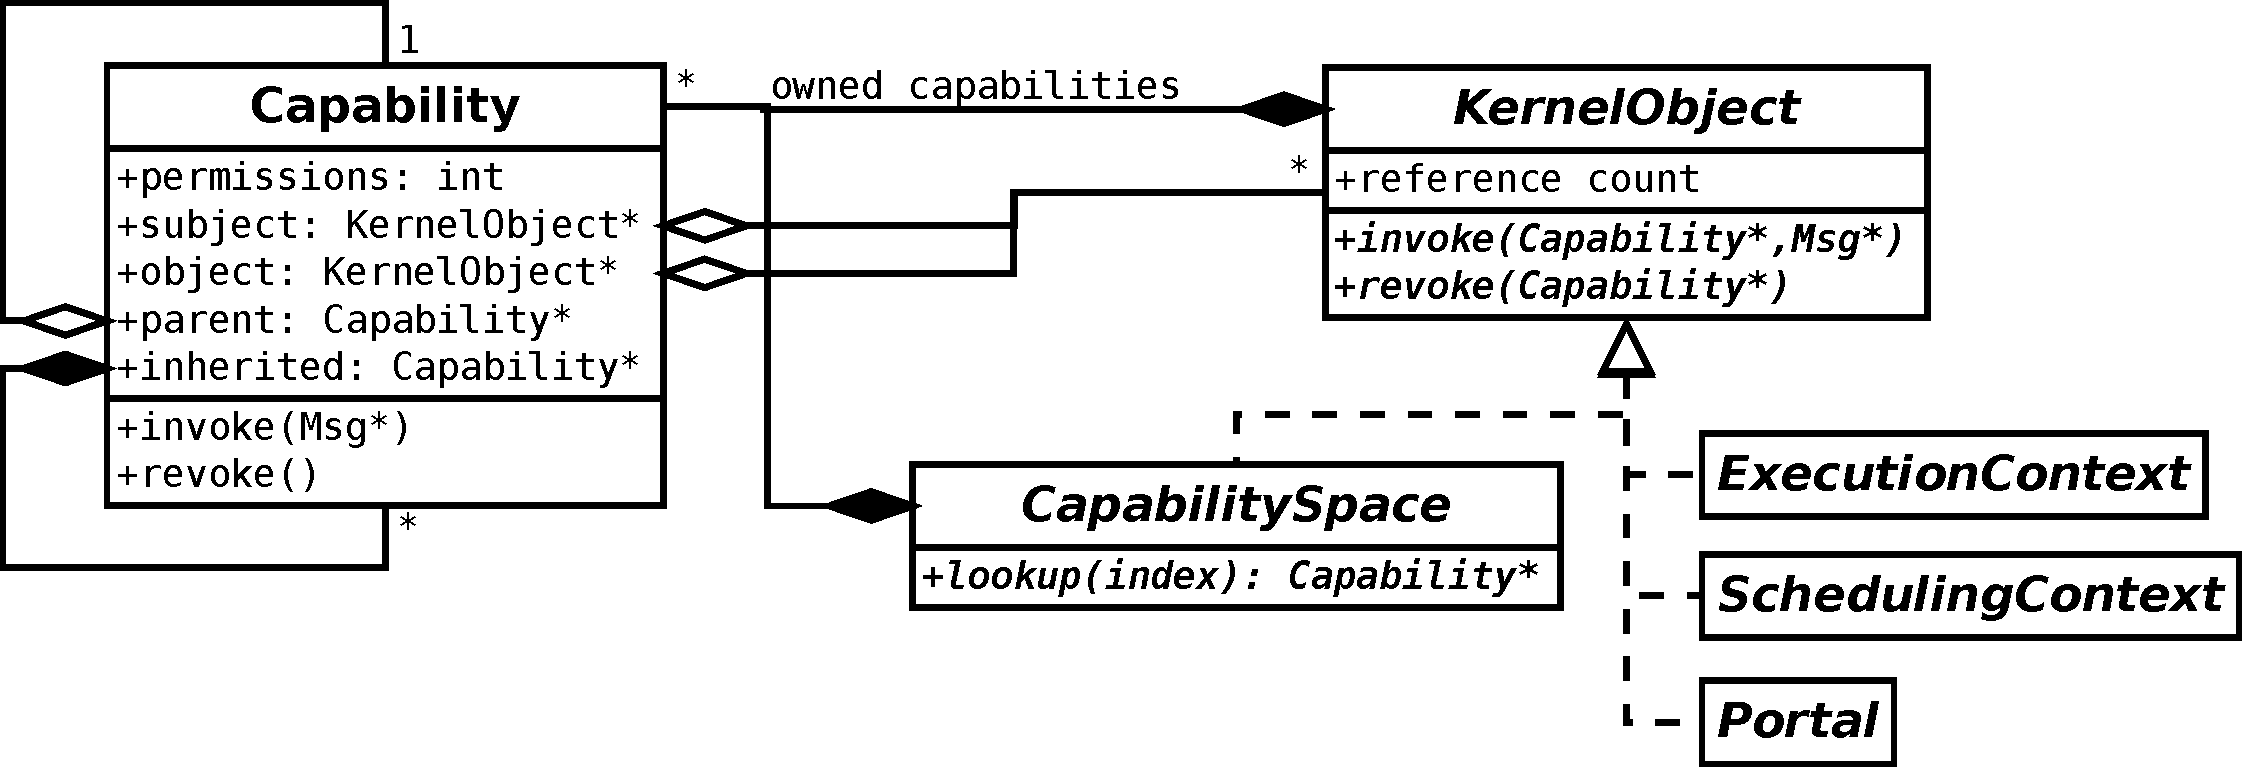
\includegraphics[scale=0.25]{fig/capability-model.pdf}
  \caption{Conceptual interactions between capabilities as smart pointers and kernel objects. The implementation stores just a subset of these pointers.}
  \label{fig:capability-model}
\end{figure}

Finally, based on the concept of object capabilities, the resource inheritance tree implements smart pointers and weak references to kernel objects in combination with tracking the object's resource inheritance. \marginnote{Sec.~\ref{sec:capability-impl}} Figure~\ref{fig:capability-model} shows a conceptual model of the interactions between capabilities and kernel objects. When a kernel object is allocated from an Untyped Memory, a respective Original Capability is created that points to the kernel object and has the Untyped Memory as parent. Therefore, the inheritance tree enumerates all objects that are contained inside the memory region and allows to force the deletion of the contained objects. Likewise, all long term references to kernel objects are stored as children inside the inheritance tree.  

The inheritance acts as a weak reference mechanism with the added benefit of being able to inform the affected subjects about the ongoing deletion. By removing all inherited capabilities, the kernel ensures on behalf of the user that no new asynchronous activities can be started on the object. On top of this mechanism, the deferred deletion support of the asynchronous objects layer ensures that objects are not deleted before all deferred activities have completed.

\begin{figure}
  \centering
  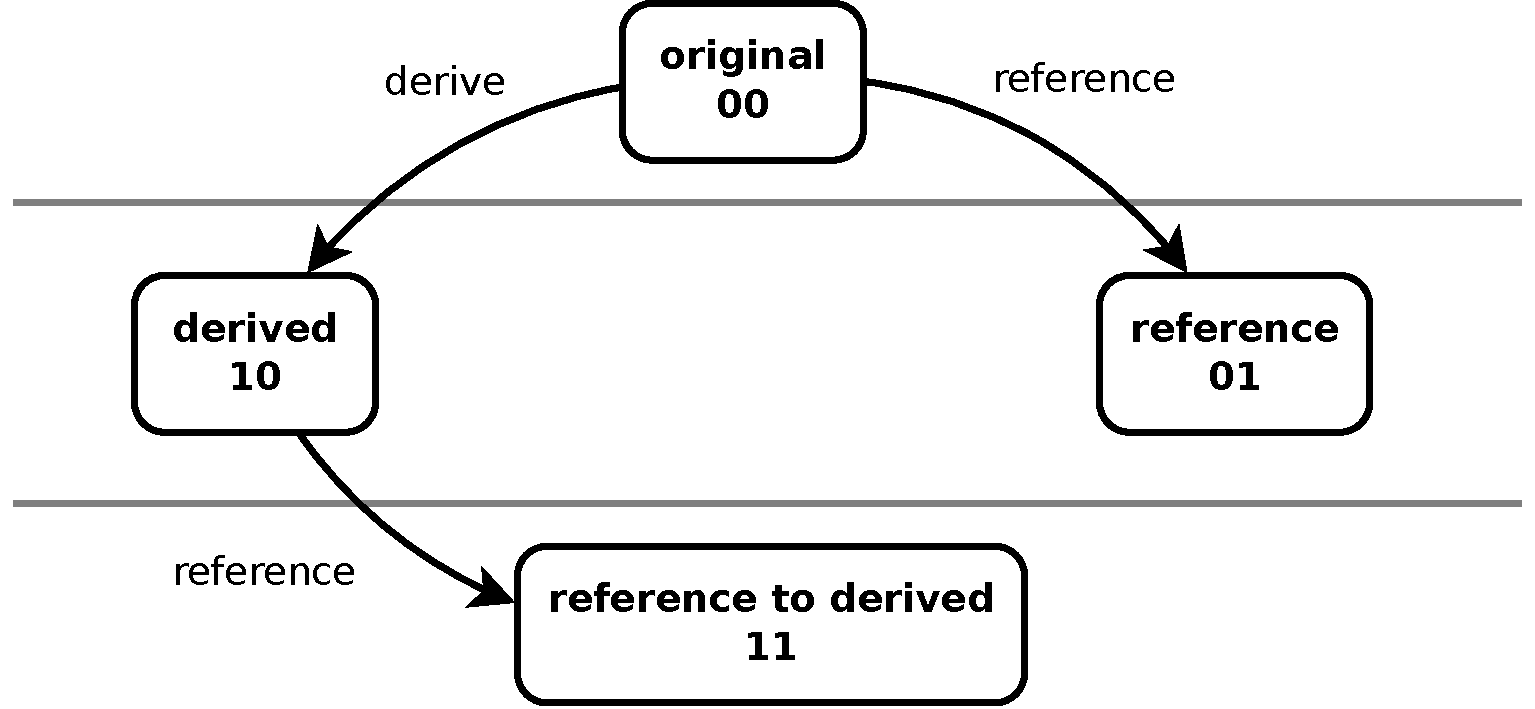
\includegraphics[scale=0.25]{fig/DerivedReferenceBits.pdf}
  \caption{Capability Types and their relations. References to derived capabilities can be revoked without revoking other derived capabilities and references to the parent.}
  \label{fig:cap-types-sem}
\end{figure}

There are four different Capability types with a different purposes. Figure \ref{fig:cap-types-sem} illustrates the four types and their relations.
Consult Section \ref{sec:capability-impl} for the role of the Capability types in implementation the Resource Inheritance Tree.

\begin{description}
\item[Original Capabilities:] \emph{manage the life-time} of Kernel Object. When a Kernel Object is created, its Original Capability is created. Whenever the Original Capability is deleted, the Kernel Object will be destroyed. As the \emph{single owner} of an Kernel Object, the Original Capability can only be referenced or derived, which creates a \emph{child} in the Resource Inheritance Tree.

\item[Reference Capabilities:]
 always are a child of an Original Capability and a weak reference to the object its parent manages. Reference Capabilities allow to \emph{share access to an original capability}, such as the right to create Derived Capabilities, without transferring the ownership of the object. Reference Capabilities can be copied, which creates another Reference Capability as a \emph{sibling} in the Resource Inheritance Tree.

\item[Derived Capabilities:] always are, like the Reference Capabilities, a child of an Original Capability and a weak reference to the object its parent manages. Unlike Reference Capabilities, Derived Capabilities cannot be copied, but only be referenced, which creates a Reference Derived Capability as a \emph{child} in the Resource Inheritance Tree. Derived Capabilities facilitate \emph{right management} by grouping references.

\item[Reference Derived Capabilities] always are a child of an Derived Capability and a weak reference to the object its Original Capability manages. Reference Derived Capabilities can only be copied, which creates another Reference Derived Capability as a \emph{sibling} in the Resource Inheritance Tree.

\end{description}

\paragraph{Discussion.}
This design is heavily inspired by the seL4 capability model~\cite{Heiser:2016:LML:2912578.2893177, GrosvenorWalker2016}, which uses capabilities as resource and access control mechanism. We solved implementation details with respect to the handling of concurrent inheritance tree manipulation and the representation of weak references to mapped frames and mapped page maps differently.
%
seL4 has Original and Derived Capabilities, but introduces a additional layer through Batched Originals for Endpoints.

The capability paradigm of Miller et al.~\cite{Miller2005} differentiates between subjects, objects, permissions, and invocations. 
\emph{Subjects} are the smallest units of computation that can hold access rights and \emph{objects} are the smallest units to which access rights can be provided. 
A \emph{direct access right} gives the subject the permission to invoke the behavior of the object.
In this sense, the kernel objects take the role of capability subjects and objects. 
The user cannot access capabilities directly, that is their instance data structures as C++ object. Instead, a capability space maps from numerical indexes to capability entries. Some capability entries are stored inside other kernel objects and can be used only indirectly. 


\subsection{Physical Memory and Address Space Management}
\label{sec:memory-impl}

Virtual memory with access control is the most important hardware-level protection mechanisms. Thus, any manipulation of the hardware's address translation tables has to be supervised by the operating system. Otherwise, applications might be able to map foreign physical memory into their own address space and compromise the consistency of the overall system. 

The current x86-64 processor architectures support up to three different frame sizes (4KiB, 2MiB, 1GiB) and the address translation employs a four-level page table structure. The following kernel object types are used to represent them:

\begin{description}
\item[Frame:] A frame represents a contiguous range in the physical address space that is backed by some kind of memory or a memory-mapped device. The range is restricted to certain sizes and respective alignment in order to reduce implementation overhead. Currently these are 4KiB, 32KiB, 256KiB, 2MiB, 16MiB, 128MiB, 1GiB, and 8GiB.

It is not useful to dynamically allocate additional kernel objects whenever smaller frames are derived from a large frame. These objects would inherit resources from \emph{both} the original Frame and an Untyped Memory, which violates the resource inheritance tree. Instead, the \emph{flyweight} pattern~\cite{gof} is used, that is Frame capabilities point to the same statically allocated Frame kernel object.

\item[MemoryRegion:] For frames that lie outside of the kernel's initial Untyped Memory, a respective base for the flyweight Frame object is needed. These are allocated as MemoryRegion objects and provide the shared Frame object for all frames that are derived from this region.  

\item[PageMap:] Each page map represents an individual table in an address space structure. Page maps are bound to a specific level during their creation. When mapping a frame or a page map into a page map's entry, the kernel checks the frame size and page map levels. One can map either a page map of the next lower level or a frame of the same level.

The top level table is called \emph{page map level 4} (PML4) and each of the 512 entries represents 512GiB of the logical address space. The PML4 entries point to \emph{page map level 3} tables (PML3 aka page directory pointer table PDP) where each entry can represent a 1GiB page or point to the next level. The entries of the \emph{page map level 2} tables (PML2 aka page directory PD) can represent a 1MiB page or point to a \emph{page map level 1} (PML1 aka page table PT), which contains 512x 4KiB pages.

\item[MappedFrame, MappedPageMap:] 
The owner of a frame retains the right to revoke the frame, which equates to unmap the frame from all affected page maps. The same is true for mapped page maps. In consequence, references from the frames and page maps to their mapped entries are needed. At the same time, page maps reference up to 512 mapped frame or page maps. This many-to-many relation has to be updated when existing mappings are overwritten, page maps are deleted, or frames are revoked. 
Therefore, \mythos page maps include the storage for one weak reference per entry and these are implemented through respective capability entries. 
Again, the flyweight pattern is used to share the kernel object between all mapped frames and mapped page maps. 
\end{description}

\paragraph{Discussion}
The seL4 implementation uses similar abstractions for Frame, MemoryRegion, and PageMap objects. Their 32-bit variant uses some clever tricks in order to fit the physical offset relative to the memory region, the virtual address, access rights, and an address space identifier into the capability's meta-data. Unfortunately, this strategy result in too large capability entries on 64-bit systems. \mythos shifts some of the information about mapped frames into the page map.

In addition, an indirection through a 2-level address space lookup table is used in seL4. This indirection is necessary because mapped frame capabilities are stored in capability spaces instead of the page map. When the address space is deleted, seL4 has thus no direct mechanism to update the respective mapped frame capabilities. Instead, they later hit on a zombie entry in the address space table. \mythos stores the mapped frame capabilities inside the PageMap kernel objects, which allows for straight forward updates. This design allows to map page maps and frames into multiple address spaces, which enables shared memory and page map sharing. The downside is, however, that storage for the weak references is wasted when just a few entries are actually mapped.

The deletion of a Mapped-type Capability does not force a \emph{TLB invalidation} on all the hardware threads that use the mapping. In implementing such an behavior would imply traversing large portions of Inheritance Tree in order to find every EC that had access to the mapping, a costly operation that would be carried out redundantly for larger address space reconfigurations.
For \emph{HPC applications}, this does not matter, as the application manages itself and is able to issue TLB invalidations only when necessary.
In other scenarios, the \emph{supervisor} that manages the address space must track all user-threads that share that the mapping and invalidate the TLB when in doubt.

Exokernels~\cite{EnglerKaashoekOToole1995} allow the user to directly read tables and only control write access. In later iterations, \mythos might allow mapping the hardware PML tables read-only in order to provides low-cost access for bookkeeping purposes.

\subsection{User Access through Capability Spaces}
\label{sec:log:capability-spaces}

% problem statement
Applications need some access path to kernel objects and not all applications should be able to access any kernel object. Hence, a translation from a per-process or per-thread name space to the process's kernel objects is needed. It should be possible to share these translation fully or partially between threads and between processes. For the compute cloud scenario, it is useful to hand access to kernel objects from the supervisor to unprivileged applications while keeping the final control of the kernel object in the supervisor. Finally, a mechanism is needed to safely delete kernel objects and revoke access rights.

% our solution
\mythos uses an object capability model that brings together the kernel-internal resource management and the various user-to-kernel translation tables. On the resource management level, capabilities are smart pointers to kernel objects combined with some meta-data about access rights and resource inheritance information for clean deallocation. The translation from user-level capability pointers to actual capabilities and kernel objects is facilitated through capability spaces. Each execution context (user thread) is assigned to one capability space. 

\begin{description}
\item[Capability Map:] In order to balance the storage consumption and the actually used name space, the capability spaces are implemented as radix trees.\footnote{aka compact prefix trees, \url{https://en.wikipedia.org/wiki/Radix_tree}} The root and intermediate tree nodes are implemented by \emph{capability map} kernel objects. 
Each capability map has a fixed power-of-2 size in order to work with static memory allocation. In addition, each map can have a guard prefix bit pattern in order to skip intermediate maps in sparse capability spaces.

\item[Capability Pointer:] The user-space applications and supervisors use \emph{capability pointers} as a numerical index into their own capability space. These pointers are a 32bit integer and the root capability map interprets the most significant bits of the pointer. First, the guard bits are checked and, if they match, they are shifted out to the left. Then depending on the map's size, the first most significant bits are used as index into the own capability entry table and are shifted out to the left as well. The capability entry points to a kernel object and the object's \texttt{lookup()} method is used to implement the recursive descend. Leave objects check that the remaining capability pointer is zero. Only the lookup method of lookup references repeats the procedure on the next lower tree node.  
\end{description}

\paragraph{Discussion.}
The node versus leave ambiguity is solved in seL4 by using a separate depth argument in system calls that manipulate the tree structure \cite{GrosvenorWalker2016}. In \mythos, the same applies to system calls that manipulate the capability map structure.


%%%%%%%%%%%%%%%%%%%%%%%%%%%%%%%%%%%%%%%%%%%%%%%%%%%%%%%%%%%%%%%%%%%%%%
\section{Physical View}
\label{sec:global-physical-view}

The physical view discusses the deployment with respect to the placement and replication of components onto processors and hardware threads as well as the basic memory layout.

\subsection{Locality Control via Monitors and Scheduling Contexts}
\label{sec:locality-control}

% problem statement
With a large number of hardware threads and non-uniform hardware topology, it becomes increasingly important to  control the placement of both data and tasks.
For example, access to remote memory in a NUMA systems can degrade  performance of a system considerately by delaying serial program phases and congesting memory interconnects.
Even worse, there are low-level operating system tasks that can only be executed on certain hardware threads: configuration registers such as the address space (CR3), devices such as the LAPIC, and configuration operations such as cache flushing and TLB invalidation can only be accessed by the affected hardware thread.

% our solution
On the asynchronous layer, locality control is exerted through the \emph{monitor} objects. Because monitors provide the interface for the asynchronous execution of method calls, they can forward these calls to kernel-level task schedulers on other hardware threads. Various policies can be implemented and configured via the monitors. This ranges from unconditional delegation to a fixed hardware thread, over load balancing across groups of threads, to opportunistic delegation~\cite{FatourouKallimanis2012} in order to improve the cache locality. The delegation to fixed threads can be used to bind operating system services to dedicated processor cores.
On the other end, monitors for purely thread-private asynchronous objects do not not need additional concurrency control mechanisms because the single physical control flow serializes the execution implicitly.

On the managed and application layers, the locality of user-level threads is controlled through the \emph{scheduling context} of an execution context. These are responsible for bringing runnable execution contexts into actual execution on an appropriate hardware thread. The scheduling context implementations use the monitor concept of the lower layers to implement these policies. The simplest variant is bound to a fixed hardware thread. All execution contexts that use such a scheduling context are run on this hardware thread. More complex scheduling contexts can implement load balancing across local groups of hardware threads. 

\paragraph{Discussion.}
\hspace{0px}\marginnote{See also~\ref{sec:multikernel-phys}}
In both multikernels~\cite{BAU09} and clustered multikernels~\cite{vonTessin_12}, sharing of kernel structures is restricted to small local subsystems such as individual threads or cores. This greatly reduces the need to further control the locality of kernel-level objects. 
Because operating system services and device driver are implemented in user mode, their placement can controlled on the level of execution contexts. Likewise, data locality for applications can be achieved by mapping local memory.

Corey \cite{Boyd-WickizerChenChenEtAl2008} allows applications to control the locality of kernel subsystems or devices by binding them to physical cores (\emph{pcores}). Moreover, control over sharing of kernel structures, such as file descriptor tables, can be use in order to exploit cache locality.

Shared memory microkernels and pure multikernels have no concept of locality: kernel objects and user threads simply exist and all inter-process communication is performed synchronously within the same hardware thread, that is within the same location. All cross-core scheduling is achieved solely at the user level via shared memory user-level communication. For example, the supervisor application on a hardware thread receives the message to schedule a specific application and, then, does a local IPC to this application. Also, supervisor applications may implement preemptive scheduling by using the local interrupt controllers in order to interrupt other hardware threads. The respective interrupts handlers switch to the local supervisor, which, then, can switch to the actual implementation.
In order to provide cross-core IPC at the kernel level, the kernel requires an own concept of locality such as the Scheduling Contexts in \mythos.

\subsection{Kernel- versus User-Level OS Services}

% problem statement
For a specific operating system service, it is often not obvious whether its more efficient if implemented inside the kernel as kernel object, inside the application as library, or as a separate user-space deamon.
Liedtke's principles for L4-style microkernels~\cite{Liedtke1996}, urge to move as much as possible outside of the kernel except for basic isolation and communication mechanisms. 
However, frequent context switching between applications, service deamons, and kernel impairs the efficiency because of the simple cores of many-core architectures.
In addition, the main challenge shifts from fast local IPC to fast coordination across cores and hardware-threads because of their large number.


% our solution
One key feature of MyThOS is the support for kernel-level services and drivers in the form of custom kernel objects. 
This allows to move performance-critical components that cannot be implemented as application-level library into the kernel. 
Due to the microkernel inheritance, the basic kernel objects are sufficient to run a fully featured software environment.
Hence, custom kernel objects are optional and should be designed based on actual performance bottlenecks.

Apart from less frequent context switches, custom kernel object might benefit from the kernel's lightweight synchronisation and communication framework. 
The flexibility is gained by two strategies: Applications interact with service deamons and with kernel objects via \emph{capability invocation} without seeing the difference. Such invocations can be processed by a custom kernel object or can be forwarded to a user-mode deamon by a portal.
On the other hand, custom kernel objects can act as proxies in order to forward kernel-internal asynchronous requests to a portal into user mode by translating them into invocation messages.

% discussion and comparison
% TODO
% User-space drivers are the core feature of L4 microkernels \cite{Heiser:2016:LML:2912578.2893177} and microkernel research is generally aimed to move not only services, but all policies out of the kernel.
% Exokernels \cite{EnglerKaashoekOToole1995} \todo{library os}
% \mythos' design enables to further explore the placement of system subsystems in kernel versus user space.

\subsection{Logical Address Spaces: Kernel versus User Space}
\label{sec:address-space-phys}

% problem statement
It is necessary to differentiate two principal types of logical address spaces. The \emph{kernel space} is used by the operating system kernel with full access permissions whereas the \emph{user space} is used by applications with user-mode execution. The construction of user spaces is supervised and restricted by the kernel in order to enforce isolation and protection between independent applications. 

Some hardware architectures switch between completely independent kernel and user address spaces on each system call. However, x86-based processors use a shared approach where each address space contains both a kernel and a user space in order to reduce the overhead of system calls. The difference is achieved by a access permission flag that protects kernel-space pages from access during user-mode execution. On x86-64 architectures, the actually 48-bit logical address space has a natural separation into a lower 128TiB half from \texttt{0x0} to \texttt{0x7FFF\,FFFF\,FFFF} and an upper 128TiB half from \texttt{0xFF80\,0000\,0000\,0000} to \texttt{0xFFFF\,FFFF\,FFFF\,FFFF}. 

% our solution
\mythos, like most operating systems, uses the upper half as kernel space and the lower half as user space. This affects the Page-Map Level 4 table (\texttt{PML4}), where just the 256 lower entries are writeable for the user-space management while the upper 256 entries have fixed values that point to the kernel-space's Page-Map Level 3 tables (\texttt{PML3} aka PDPT). These are shared across all hardware threads and are rarely modified by the kernel as discussed in Section~\ref{sec:kernel-space-management}. When creating PML4 objects, the upper 256 entries are directly filled with the kernel space default entries. Therefore, later manipulation of the kernel space is transparent to all address spaces and does not require to touch every PML4 object.

\paragraph{Discussion.}
Some operating system designs propose a single-address space approach for the applications. There, all applications share the same address space layout, that is the same translation from logical to physical addresses. Just the access permisions vary between the applications. One advantage is, that pointers are globally unique because all applications see the same memory at that address. One example is Multics, which used segments to describe access permissions and the segment selector was part of the pointers instead of separate registers like on x86.

On x86 architectures in 32bit mode, segments can be used to put multiple applications into the same logical address translation while hiding this fact from the application's code~\cite{SomaGerofiIshikawa2014}. However, x86-64 in 64bit mode simply ignores the base addresses of code, data, and stack segments because almost all operating systems were not using segments anyway.

\subsection{Kernel-Space Memory Management: Physical Memory}
\label{sec:kernel-space-management}
% problem statement
In order to be independent of the user address space layout, the kernel has to map the memory of all kernel objects and everything that is accessed from within kernel-mode execution into the kernel space. Access to user space addresses is possible in principle but requires to track which address space the address belongs to and handle page access exceptions. All objects and data structures need to placed appropriately into the kernel space, \marginnote{Sec.~\ref{sec:boot-dyn}} whether they are created during the boot sequence or dynamically allocated and deallocated during the system' lifecycle.

% our solution
All of the kernel's memory allocation is facilitated through Untyped Memory kernel objects. Based on the firmware's memory map, the initial untyped memory is created and, then, used to allocate all initial data structures---not just initial kernel objects. The remaining untyped memory is passed via a capability to the root application.

The kernel-mode code operates on physical addresses. This removes the need to establish dynamically kernel-space page tables, which would require a kernel-space memory management for the on-demand allocation of page table structures. Of course, the processor architecture does not allow to access the physical addresses directly. Therefore, a contiguous \emph{direct mapped range}, similar to an identity mapping, is initialised in the kernel-space during the boot sequence. Physical addresses are accessed by using them as offset into this range.

This direct mapping segment covers the whole physical memory or at least a large enough portion to provide space for the later kernel objects. The covered range is handed as untyped memory to the user. Any additional memory is handed as frame objects to the user. This ensures, that the kernel can directly access all kernel objects without having to fear page access faults.

The kernel can implement an optional memory protection scheme in order to detect bugs earlier. Most parts of the direct mapped range are read\&write protected until they are explicitly used for allocation via an untyped memory or via a temporary access to specific physical addresses. This requires separate tables with reference counters in order to prevent revoking access concurrently. These reference counters are held per 2MiB page. Access to smaller objects is simply extended to the enclosing 2MiB aligned range.

The only user-space memory that is accessed by the kernel are the portal's invocation buffers. Here, seL4's strategy is applied in order to avoid all the hassles with kernel-mode page faults: the kernel accesses the buffer directly via its physical address, which is known through the frame object that was registered as buffer at the portal. The user maps the same frame into its user-space. Additional care is necessary to differentiate frames inherited from untyped memory against frames that are not accessible via the kernel's direct mapped range. When registering a buffer frame at a portal, the portal has to check whether the physical address range lies within the direct mapped range. Alternatively, the frame capabilities can contain a kernel access flag that shows which frames are accessible to the kernel.

Custom kernel objects might need to access additional regions of the physical address space, for example to implement device drivers. These ranges are not part of the direct mapped range and, hence, mapping them into the kernel space requires dynamic allocation of page table structures. Note that the mapping is created on user request during the creating of these custom kernel objects. Hence, the user can provide the needed untyped memory.

\paragraph{Discussion.}
Linux and Unix-based systems have to deal with kernel-mode access to user-space addresses because of the design of many system calls from the POSIX interface. First, each access to user space was protected by a software-implemented page table walk to check whether the address is accessible. This proved to be very slow and mostly unnecessary. In addition, it is not secure against concurrent manipulation of the page tables. Thus, the Linux kernel replaced these checks with a lazy page fault strategy. Just a selected set of functions implements user-kernel data transfers. The page fault interrupt handler checks whether the faulted instruction is part of one of these functions and, in this case, jumps to a respective handler code, similar to the C++ exception mechanism. While efficient and effective, this approach does not answer what the kernel should do when such a page fault happens. It increases the number of possible error conditions that have to be handled by the kernel. 

The differences between synchronous and asynchronous IPC are quite relevant for non-local communication. Support for unbounded asynchronous IPC messages, like in Mach, would require dynamic memory management for the unbounded cross-core message queues. Instead, \mythos provides just bounded asynchronous communication in the form of deferred synchronous IPC via pre-allocated portals. The number of messages in flight is bounded by the existing portals and all necessary data structures were allocated together with these portals.     

\subsection{Core-Local Memory: FS/GS Segment Base}
% problem statement
Multiple hardware threads share the same kernel-space address layout. However, each hardware thread requires a few thread-specific data structures such as local task queues and state information about the currently active user thread or execution context. Global variables, that is outside of function bodies and class definitions, and static member functions cannot be used for these structures because, then, all hardware threads would access the same instance instead of their own. Hence, a fast lookup mechanism is needed that translates logical identifiers into the respective hardware-thread-local instances.

% our solution
This situation is very similar to thread-local storage in application threads and uses the same hardware support. The main difference is, that the kernel's core-local memory is relative to the physical position, that is the hardware thread, whereas the application's thread-local storage is relative to the logical control flow, that is the execution context.

\mythos uses the base address of the x86 architecture FS and GS segments. This enables fast access to thread-local storage via segment-relative load and store instructions. For historical reasons, the segment descriptors can only hold 32-bit base addresses. These can be used as thread-specific 32-bit offset with the logical identifier as 64-bit base. However, special model specific configuration registers in x86-64 processors allow to override the segment descriptor's base address with a 64-bit address.

The base kernel requires only a limited set of core-local variables that are known at compile time. Because the maximal number of hardware threads is also known when linking the kernel image, a sufficiently large core-local memory segment is reserved in the kernel image. The static addresses to these core-local variables point to the instances of thread 0. The GS segment base contains a 32bit displacement for the hardware thread's instances. Any GS-relative memory access to core-local variables thus uses the sum of the first thread's address to the variable and the actual thread's GS displacement. 

This strategy does not require additional address mappings in the kernel-space. In principle, dynamic allocation of additional core-local variables is possible: Unused parts of the linked core-local segment can be used and additional segments can be allocated from untyped memory at run-time. This works because the GS base address always is a displacement offset relative to the beginning of such segments.

\paragraph{Discussion.}
Several options are available to implement such local storage lookup. Basically, the global logical identifiers are an offset into a thread-specific address range. On some architectures, the compiler reserves a register and this contains all the time the fixed thread-specific base address. Unfortunately, this wastes an expensive register that is more useful for actual computations. The thread-specific base address can also be placed at the bottom of each stack and by limiting the stack size and alignment, the bottom's address can be calculated from the current top of the stack. This costs additional computations and memory lookups while constraining the stack size. 

Core-local memory is used by all shared memory operating system kernels. The multikernel design avoids this issue by using a separate kernel address space per hardware thread, which makes all global and static variables core-local. Nova seems to use a dedicated address range in the kernel space. This range is mapped to different physical memory for each hardware thread and, thus, static variables in this range are core-local. However, this prohibits the sharing of PML4 tables across hardware threads. Either, the user would have to create separate page tables on each hardware thread like in a multikernel or the kernel would have to allocate and synchronise core-local PML4 tables implicitly for each logical address space.
 

\subsection{Multikernel Support}
\label{sec:multikernel-phys}
% problem statement
What is needed in order to implement a multikernel or a clustered multikernel based on \mythos? In a multikernel, each hardware thread runs its own kernel instance and does not share kernel objects with other hardware threads. Hence, no concurrency control is needed except for dealing with interrupts. A clustered multikernel shares a kernel instance in a small group of hardware threads. This balances the utilisation of locally shared hardware resources such as caches and TLB versus the contention caused by concurrent kernel activities. 

% our solution
The kernel instance is defined completely through its kernel address space layout. Multiple instances can be created during the boot sequence \marginnote{Sec.~\ref{sec:boot-dyn}} by creating multiple kernel space page tables. The kernel's code segment can be shared because it is read-only. The kernel's segment for global variables and static object instances has to be mapped to separate physical memory and initialised by copying from the first hardware thread. Similarly, the segment for the core-local memory needs to be replicated and mapped to separate physical memory. Finally, the direct mapped range is replicated but maps to the same physical addresses. Mutually exclusive use of this memory is ensured via separating the untyped memory per kernel instance. The kernel trusts the user-mode supervisor to not share the untyped memory across kernel instances.

The supervisor on top of each kernel instance is responsible for establishing shared user-space memory across kernel instances for communication and to implement remote capability transfers. When receiving a frame capability, the respective untyped memory range has to be converted into a local frame kernel object. This is simplified by handing the complete untyped memory range to all supervisor instances and let them coordinate who is using which part. 

% discussion and comparison
% TODO?

%%%%%%%%%%%%%%%%%%%%%%%%%%%%%%%%%%%%%%%%%%%%%%%%%%%%%%%%%%%%%%%%%%%%%%
\section{Dynamical View}
\label{sec:global-dynamical-view}

This section focuses on interactions inside the kernel, between applications and kernel, and between applications as well as the life-cycle management of components and the necessary scheduling.

\subsection{Error handling: IPC Messages to Supervisor}
\label{sec:error-dyn}

% problem statement
The error handling differentiates between asynchronous exceptions and synchronous errors. Asynchronous exceptions preempt the execution of user- or kernel-mode execution and jump to the kernel's interrupt handling. Synchronous errors are detected by assertions during normal operation, for example when a system call fails due to insufficient access rights.
Both situations require a recovery strategy that forwards the exceptions and errors to appropriate handlers.

% our solution
Synchronous errors appear during system calls or are related to (deferred) synchronous calls. They are passed to the application via a normal system call return with the error encoded in the return values.

Asynchronous exceptions arise from interrupts, processor traps, and all faults that cannot be tracked back to a synchronous system call. Exceptions during user-mode execution are transformed into an invocation message and sent to a \emph{exception handler kernel object}. This object is selected based on the affected execution context and is configurable. The basic variant uses a portal that activates an execution context, which can be used to implement supervisor hierarchies. The user-mode handler receives the exception message, can inspect and handle the causes and optionally restart the affected execution context.

Because of concurrent state changes, exceptional situations can occur during kernel-mode execution. These are detected through assertions like synchronous errors but cannot be associated with a specific, currently active system call. For example, a response message can hit a revoked or mis-configured client portal. This exception is not interesting for the server side and, thus, has to be handled by the client's exception handler in the same style as asynchronous exceptions.

\paragraph{Discussion.}
Unix systems use a signal mechanism to jump into a handler function in the context of the affected thread. Signals are used for both asynchronous exceptions, for example the kill signal, and synchronous exceptions, for example a memory protection fault. This forced jumps inside a single user thread pose some serious problems with respect to stack space and interrupt-alike preemption. 
Windows NT uses separate handler threads for asynchronous exceptions. Synchronous exceptions are translated into localised signal handlers very similar to the C++ exception mechanism but with the option to retry the affected instruction.
\mythos, like many microkernels, hands control over the exception handling to supervisors instead of implementing a fixed policy. This exception handler could then, for example, implement the affected execution context's jump to an exception code like in Windows or C++.
% TODO: citation for supervisor hierarchy


\subsection{Concurrent Object Deallocation}
\label{sec:async-deletion-dyn}

% problem statement
In a concurrent system, races between object usage, such as method calls and access to member variables, and object deallocation can easily occur.
\marginnote{See also~\ref{sec:log:capabilities}}
The capability-based weak references mechanism cleans up long-term references before any object deallocation. However, temporary references in messages and concurrent control flows, for example between capability lookup and using the object, could still lead to race conditions and premature deallocation.

% our solution
Our solution delays the destruction of objects until all temporary references and in-flight messages are cleared. First, kernel objects are deallocated only when the Untyped Memory they were allocated from is recycled. Before this happens, all long-term references are cleared through revoking all inherited capabilities in the resource inheritance tree.

In order to deal with outstanding messages, pending responses, and references contained inside in-flight messages, the kernel object's Monitor
\marginnote{See also~\ref{sec:concurrency_control}}
tracks both the number of temporary references and pending messages of the object. Object destruction is facilitated through an asynchronous method and the Monitor executes this call after all temporary references and pending messages are finished. Because all references on the capability layer are already revoked, no new temporary references or pending messages can be created.

This leaves short-term references in concurrent kernel control flows. For example, another hardware thread could have successfully looked up the object pointer before the capability was revoked but still have not issued its request and, hence, is invisible to the object's Monitor. To resolve this race between a thread increasing the counter after reading a soon deleted capability and the deallocation of the object, the memory is only recycled after all hardware threads have either left the kernel or returned to the task scheduler once.

A hardware thread that is not inside the kernel can hold no short-term references. Likewise, returning to the hardware thread's task scheduler ensures that all activities that could have held a short-term reference have completed and have updated the Monitor's reference count. This situation is detected lazily by scheduling a tasklet at every hardware thread that is in the kernel at the time of the Untyped Memory's recycling and waiting for the execution of these tasks. To this end, a broadcast ring of asynchronous objects is used. Hardware threads that are not currently inside the kernel are skipped in order to avoid waking up sleeping threads or needlessly interrupting applications.

% discussion and comparison
\paragraph{Discussion.}
Reference counting is a well-known concept for lifetime management of objects. The employed approach is very similar to the Deutsch-Bobrow method of reference counting.\todo{cite}
One major problem of reference counting in a non-distributed context are cyclic references that are usually avoided by using weak references to break the circle.

In \mythos, the general lifetime of an object is managed by the original capability, and all other capabilities are basically weak references. However, as capabilities are not counted, creating an temporary reference or entering the Monitor races with the destruction of the object.
%
To resolve this race, the broadcast-based mechanism has been introduced.
This mechanism is very similar to \emph{basic RCU deletion schemes}~\cite{McKenney2004, McKenneyWalpole2007} which delay the deletion of copies by rescheduling on every hardware thread. If frequent recycling of Untyped Memory is needed, enhanced RCU schemes may provide further ideas on how to increase the throughput.

Multikernels like Barrelfish prohibit shared kernel objects and, hence, no invisible temporary references should exist. Similarly, seL4 and clustered multikernels use a big kernel lock to prohibit concurrency inside the kernel, which eliminates data races.

\subsection{Credit-based Flow Control}
\label{sec:credit-flow-dyn}

% problem statement
The amount of memory in many-core architectures is quite small in relation to the number of hardware threads. With asynchronous programming models, an even larger number of logical control flows exists.
Therefore, assigning each control flow a practically infinite, hence ``large enough'', message/context buffer is not feasible. Conversely, dynamic memory allocation for buffers injects additional runtime dependencies  and, thus, latencies into the communication.
Last but not least, the \emph{system throughput is limited} by the maximal throughput of the interconnect and the maximal throughput of the execution units. Once one of them is saturated, being able to create further messages or control flows does not increase the overall throughput any further.

% our solution
In \mythos, these difficulties are avoided by incorporating the statically allocated bounded message buffer into the design of the asynchronous objects model:
\hspace{0px}
\marginnote{See also~\ref{sec:concurrency_control}}
\emph{Tasklets} serve both, as a \emph{buffer} to hold a message or a control flow context, and as a \emph{token} to implement \emph{credit-based flow control}.
Because each call to an asynchronous method consumes a Tasklet, the number of messages and control flows originating from a single asynchronous object is bounded by the number of Tasklet that it owns. New asynchronous activities can be started only after the Tasklet was returned through a call to a response method.
Passing the Tasklet is \emph{explicit and visible to the programmer}. This forces the designers and developers to reason about the implications of asynchronous calls.

Inside asynchronous objects, the passed tasklet is used to store all information about the issued method call. The tasklet is scheduled through the object's Monitor for mutually exclusive execution and the actual implementation of the called method calls an asynchronous response method on the caller's continuation object in order to pass along or return the Tasklet and flow control credit.

A more complex Monitor is needed if incoming asynchronous requests lock object-internal resources such as additional Tasklets for parallel communication with multiple other objects. In this case, new requests can be executed only after the previous request is completed, that is after the request's processing received all internal asynchronous responses. In such situations, a Monitor implementation is used that queues incoming new request separate from incoming response messages. Response processing is prioritised and the oldest of the pending requests is executed only after the previous request was declared as finished.     

\paragraph{Discussion.}
In TinyOS, the server objects have to supply the task objects for bounded asynchronism, which simplifies the flow analysis. However, in multi-threaded environment, the concurrent client requests would, first, have to allocate one of these task objects via a wait-free dispatching data structure and, then, have to enqueue the task to a shared wait-free scheduler queue. \mythos uses static allocation of Tasklets at the client object in order to reduce the need for dynamic dispatching. Many simple asynchronous object own no or just a single Tasklet.


\subsection{Portal: States and Operations}
\label{sec:portal-dyn}

%problem statement
Capability invocation is the main mechanism for user-mode applications to interact with the kernel objects and to initially communicate between applications/processes, for example between worker process and supervisor. Portals \marginnote{See also~\ref{sec:kernel-objects}} are the key component for capability invocation and inter-process communication. This section describes the system calls that enable sending and receiving invocation and discusses the Portal's respective life cycle.

\begin{figure}
\begin{center}
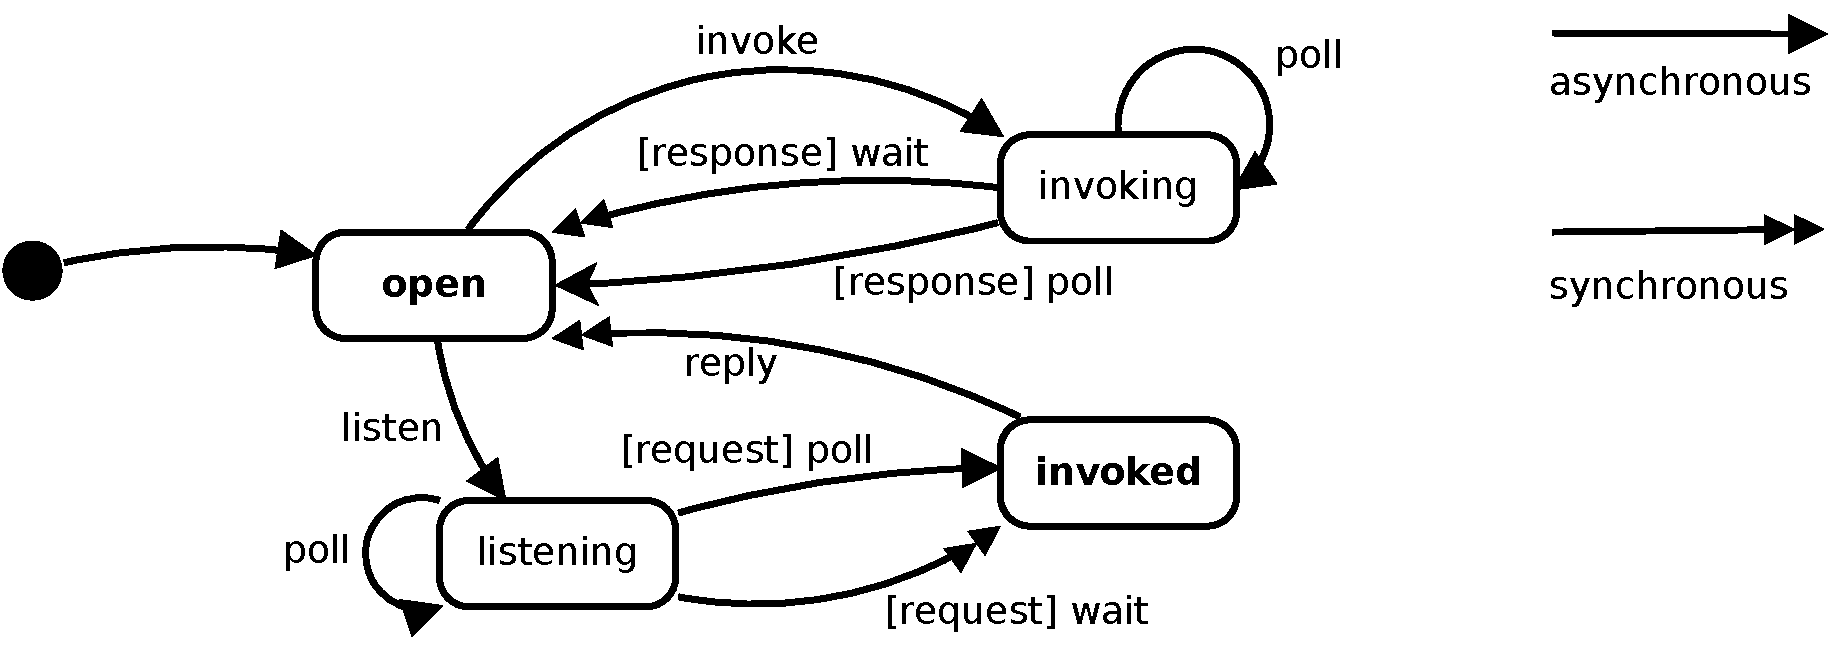
\includegraphics[scale=0.25]{fig/portal.pdf}
\caption{User-visible states of the Portal object.}
\label{fig:portal:state}
\end{center}
\end{figure}

Figure~\ref{fig:portal:state} shows the Portal's states and transitions. Initially, the Portal is in the \emph{open} state and can be configured to either listen for incoming requests or to send a request in the form of an invocation message. The Portal returns to the \emph{open} state by sending a reply in the \emph{invoked} state or by receiving a reply from the \emph{invoked} state. The \emph{invoke}, \emph{listen}, \emph{wait}, and \emph{reply} transitions are triggered through system calls of the Portal's owner. The synchronous transitions return from the system call after the operation completed whereas the asynchronous variants return immediately. 

The message data is stored in an \emph{invocation buffer}, which is shared memory between the application and the Portal on the kernel side. Applications should write to the invocation buffer only when the Portal is in the \emph{open} or \emph{invoked} state. However, this is not enforced by the operating system because non-conforming applications would just interfere with their own operation. The kernel objects that read from the invocation buffer first copy the needed values before checking their validity. Hence, concurrent manipulation of the invocation buffer is ignored.

The following system calls directly interact with the owner's Portal. For convenience and in order to reduce the number of system calls, combined system calls such as \emph{invoke+wait} are available.

\begin{description}
\item[invoke(portal, uctx, dest):] the content of the invocation buffer is sent asynchronously as an invocation to the specific destination \texttt{dest}, which is a capability pointer into the caller's capability space. In general, any kernel object that implement the invoke operation is a valid destination. When used for communication between applications, the destination will be a Portal. The \emph{user context} \texttt{uctx} is an opaque pointer (64bit integer) that is returned by \texttt{wait()} and \texttt{poll()} on arrival of the reply. It is used by the user-space runtime environment to associate received messages with the respective communication channel.
 
\item[listen(portal,uctx):] this asynchronous operation switches the portal to receive mode and allows the Portal to write into the invocation buffer. Otherwise, only the application is allowed to write. Again, the user context \texttt{uctx} is returned by \texttt{wait()} and \texttt{poll()} when a request was received.

\item[reply(portal):] is a synchronous operation that returns after the invocation buffer is copied into the other side's invocation buffer. The operation will succeed quickly because the other side has to wait for the reply already. If the other side's Portal is not ready to receive the response or does no longer exist, the reply operation fails immediately. This ensures that misbehaving clients cannot delay the supervisor's control flows.

\item[bind(portal,ec):] rebinds the Portal to a different Execution Context, which will receive future invocation and reply messages of the Portal. This operation can be issued in any state and just selects the Execution Context that will be resumed by incoming messages. There is a race between rebinding and receiving a message. Whichever is processed first decides which Execution Context handles the message. However, applications that perform rebind in such a receiving state should be prepared to handle the message in both Execution Contexts anyway.   

\item[wait()$\rightarrow$uctx:] is a synchronous operation that blocks until a message on any Portal bound the Execution Context has arrived. The message can be either a invocation or a reply, and may has been arrived on any portal that is in the \emph{listening} or \emph{invoking} state. The user context \texttt{uctx} of the respective \texttt{listen()} and \texttt{invoke()} calls is returned. The \texttt{wait()} call can be interrupted without receiving any message. In that case the value 0 is returned as user context and the error number is set.

\item[poll()$\rightarrow$uctx:] works like \texttt{wait()} but returns immediately if no received messages were pending.
\end{description}

The combination \texttt{invoke+wait} is synchronous and returns when any message was received on one of the execution context's Portals. In contrast, \texttt{invoke+poll} is asynchronous and returns immediately. If a received message was pending in one of the Portals, the respective user context value is returned.

Note that \emph{poll} races with enqueuing a message on the Portal. If a application requires not to miss an incoming message, it must use \emph{wait} instead.

\todo{explain send-wait-reply-wait sequence}

\todo{how to remove in-flight messages when the sender's capability to the destination is revoked before delivery?}

% TODO discussion

\subsection{Execution Context: States and Operations}
\label{sec:execution-context-dyn}

% problem statement
Execution Contexts \marginnote{See also~\ref{sec:kernel-objects}} represent user-mode application threads by combining a reference to a logical address space, a reference to a capability space, a reference to a scheduling context, and an interface to the user-mode processor state such as register contents. The execution state is modified by three factors: synchronous system calls, synchronous exceptions/traps, asynchronous preemptive interrupts. This section describes the life cycle of Execution Contexts and their interaction with communication and notification mechanisms.

\begin{figure}
\begin{center}
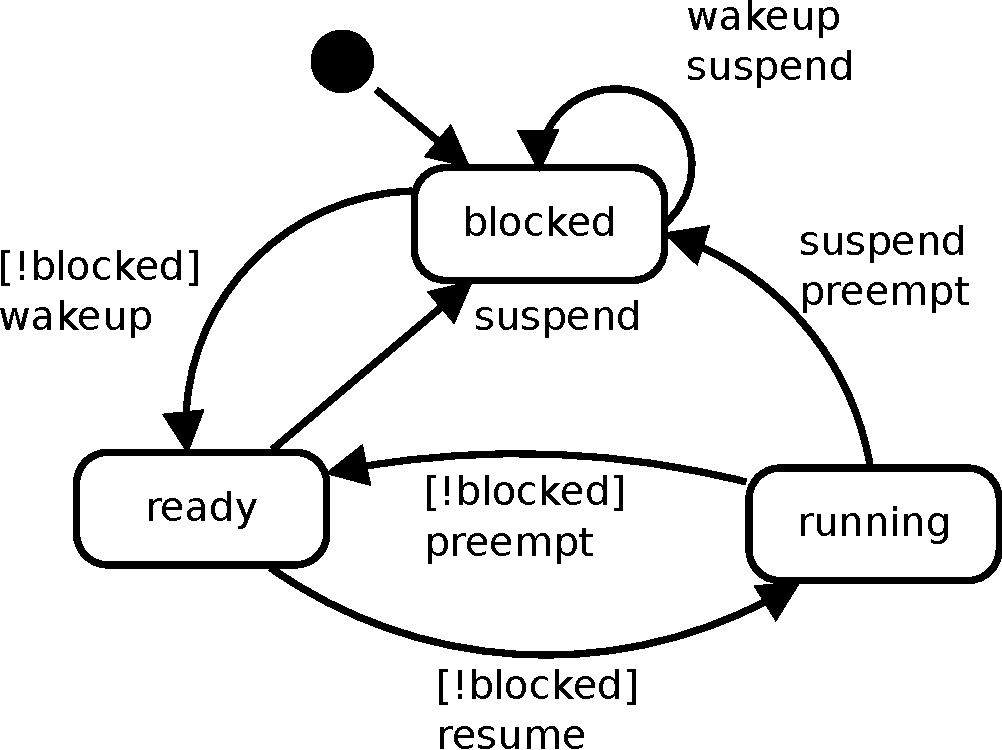
\includegraphics[scale=0.25]{fig/ExecutionContext.pdf}
\caption{State machine for an Execution Context.}
\label{fig:portal:state}
\end{center}
\end{figure}

% our solution
Figure~\ref{fig:portal:state} summarises the states and transitions of Execution Contexts. Initially, the Execution Context is \emph{blocked}. When it transitions to \emph{ready}, the associated Scheduling Context is informed, which is responsible to schedule the Execution context on a hardware thread. Once this hardware thread returns from the kernel mode into the Execution Contexts user-mode execution, the state changes to \emph{running}. An Execution Context can be in this state only on a single hardware thread at any time. When the hardware thread enters the kernel again, the Execution Context's state transitions into the \emph{blocked} or the \emph{ready} state.

Synchronous system calls enter the kernel-mode execution from the Execution Context's user-mode thread and the Execution Context is blocked until the call has completed. The main set of system calls is presented in Section~\ref{sec:portal-dyn}.
Synchronous exceptions and traps are caused by the user-mode execution, enter the kernel, and block the Execution Context until the exception is handled. The exception handling is discussed in Section~\ref{sec:error-handling}.
Asynchronous preemption is caused by interrupt signals received from devices and by inter-processor interrupts (IPIs) that were sent from other hardware threads. This enters kernel mode as well but does not automatically block the Execution Context. 
Finally, an Execution Context can be marked as blocked via an invocation message, for example, from a supervisor. This does not interrupt the running execution but prevents any future return to user mode from interrupts, exceptions, or system calls.  Therefore, a supervisor should first block the execution context and then raise an IPI in order to suspend a Execution Context preemptively.

In conclusion, a number of distinct reasons can block the Execution Context and multiple reasons may overlap. A field of \emph{block flags} is used to represent these reasons. Only after all block flags are cleared, the Execution Context transits into the \emph{ready} state. Therefore, after each update of one of the block flags, the overall state is checked. The following block flags are used:

\begin{description}
\item[No Scheduling Context:] This flag is set when the Execution Context was not yet bound to an Scheduling Context or the Scheduling Context was revoked. Without a Scheduling Context, the kernel does not know how and where to run this Execution Context.
\item[No Address Space:] This flag is set when the Execution Context was not yet bound to an Address Space or the Address Space was revoked. Without an Address Space, the kernel cannot switch into the correct logical user address space.
\item[Faulty] This flag is initially set to show that its processing state is not fully configured. It is also set by synchronous exceptions and cleared by the exception handler. Any supervisor that holds a reference to the Execution Context can set this flag in order to prevent its execution.
\item[Waiting] This flag is set by the \texttt{wait()} system call and is cleared when an associated Portal receives a message.
\end{description}

Execution Context are not blocked when no Capability Space was assigned or it was revoked. Without a Capability Space, almost all system calls will fail. However, the system call entry code has to check for the presence of a Capability Space anyway. It might happen that some application or supervisor revokes a Capability Space while threads are still using it. In this case, the next system call has to detect the missing capability space and has to fail gracefully.   

The implementation of Execution contexts uses a more general internal interface to the block flags based on bit fields and masks. The following methods are available on Execution Contexts. Not all of them are accessible through invocation messages. 

\begin{description}
\item[suspend(bitfield)$\rightarrow$bitfield:] or-combines the old block flags with the given bit field and returns the old flags. When this blocks the Execution context from the \emph{ready} state, no additional action is needed. The Scheduling Context checks the block flags before switching to the \emph{running} state. While in \texttt{running} state no preemption is done automatically. This can be issued by the supervisor separately.

\item[wakeup(bitmask)$\rightarrow$bitfield:] resets the block flags according to the given mask. If the block flags are all cleared, the Execution Context is scheduled via the \emph{Scheduling Context}.

\item[isRunnable()$\rightarrow$bool:] returns true if none of the block flags is set.

\item[preempt():] if the Execution Context is in the \emph{running} state, a kernel-internal doorbell interrupt is sent to the hardware thread that currently runs the Execution Context. The preemption request is handed to the respective Scheduling Context, which uses the kernel's asynchronous infrastructure to issue the interrupt signal.

\item[dequeue():] if the Execution Context is enqueued for execution in a Scheduling Context, this operation removes it from the queue. The implementation reuses capabilities as queue and weak reference mechanism in cooperation with the Scheduling Contexts. 
\end{description}

In order to forcefully stop an Execution Context, its supervisor has to first set one of the block flags and then send a preemption. Normally, this would return from the user-mode execution into the kernel and, then, see the block flag in order to not reschedule the Execution Context. However, the targeted Execution Context could have been scheduled for execution without running yet. Hence, the Scheduling Context has to check the block flags before switching to the user mode.

There is potential for a race condition between running, blocking, and preempting the Execution Context. Either the preemption could be dropped because the thread is not running yet or the blocking reason could be missed because the thread already runs. This is resolved as follows: The target hardware thread first sets the state to \emph{running} and then checks the block flags. The other side updates the block flags first and then calls \texttt{preempt()}, which looks for the \emph{running} state.

The \texttt{dequeue()} is not necessary during normal operation, because Execution Contexts that became blocked after enqueuing are ignored lazily. However, rebinding to a different Scheduling Context and deleting Execution Contexts require an immediate mechanism.

% TODO discussion

\subsection{Interrupt Handling and the Scheduler Monitor}

% Die interrupt handler müssen rausfinden können, ob sie die ersten im kernel sind oder nicht. Wenn sie die ersten sind, sind sie für die Aufgabenabarbeitung zuständig, ansonsten erzeugen sie nur Epiloge in Form von Tasklets.
% Der Monitor muss auch durch die Systemcalls betreten werden, spätestens wenn sie anfangen wollen, Tasklets abzuarbeiten. bei syscall_leave wird dann auch der monitor verlassen.
% Der Monitor ist eine core-locale variable, kein big kernel lock.

\subsection{Monitor Example}


This section describes the interface and dynamic behavior of a homed monitor with separate \emph{request} and \emph{response queues}. All asynchronous methods protected by the monitor are executed on a specific hardware thread, the \emph{home place} of the monitor. The monitor prioritizes response messages in order to prevent blocking to many in-object resources with requests.

\begin{description}
\item[request(tasklet, function)] increases the request counter atomically by one. If the counter has been zero, this request uses the supplied tasklet to schedule the function at the home place. Otherwise, it enqueues the function on its internal \emph{request queue}
\item[response(tasklet, function)] increases the request counter by one and uses the supplied tasklet to schedule the response method on the home place. If the counter has been zero, this response uses the supplied tasklet to enqueue the function at the home place. Otherwise, it enqueues the function on its internal \emph{response queue}.
\item[requestDone()/responseDone()] atomically decreases the request counter by one. If the response counter reaches zero, there are no pending requests and responses. Otherwise, it first checks the \emph{response queue} and schedules it the response if any is found. If there is no pending response, a pending request from the \emph{request queue} is scheduled on the home place.
\item[acquireRef()] increases the reference counter by one.
\item[releaseRef()] decreases the reference counter by one. If the reference counter reaches zero, there are no further references.
\end{description}

\paragraph{Discussion.}
The monitor presented here provides concurrency and locality control by allowing execution only on its home place. 
More sophisticated monitors may support delegation locking schemes in order to relax the locality constraints, or reader-writer synchronization. Additional waiting queue can be added in order to support condition variables.


\subsection{Kernel Entry and Exit}
\label{sec:entry-dyn}

There are various reasons why a user-thread may enter the kernel: synchronous and asynchronous system calls, hardware exceptions (traps) or interrupts.
Fortunately, on implementation level, there are only two main mechanism to enter the kernel: interrupt and system calls. In the rest of the section, both are called an \emph{entry event}.

In \mythos, the only the information required to continue the execution of a user-thread is the processor state. As described in Section \ref{sec:execution-context-dyn}, a Execution Context can even be blocked for multiple reasons at once.
However, the entering reason determines what processor state is expected by the user-level code when it continues running.
For a \emph{system call}, it is expected that the processor state is \emph{modified} to reflect its return value. This further implicates that the value to be stored depends on the system call and reflects what may be returned.
\emph{Portal operation system calls} \marginnote{See also~\ref{sec:portal-dyn}} can either return no value, an error code, or a user context pointer.
For example, \emph{wait} and \emph{poll} operations on a Portal are expected to return a \emph{user context}, whereas other portal operations will only return error codes. 
For an \emph{interrupt}, it is important that the saved processor state is \emph{preserved}.

\begin{table}
\begin{center}
\begin{tabular}{l|ll}
\toprule
 & blocking & non-blocking \\
\midrule
interrupt & page fault & hardware timer \\
system call & invoke (async.) & wait (sync.) \\
\bottomrule
\end{tabular}
\caption{Combinations of different entry methods and blocking semantic.}
\label{tab:entry_block}
\end{center}
\end{table}

\mythos separates blocking from the reason the kernel has been entered.
As illustrated in Table \ref{tab:entry_block}, the method of entering the kernel and blocking are to two separate concerns and can occur in various combinations.
Moreover, a Execution Context might enter the kernel for a non-blocking reason, but is concurrently suspended by its supervisor.

\paragraph{Entry Event Handling}

\begin{figure}
\begin{center}
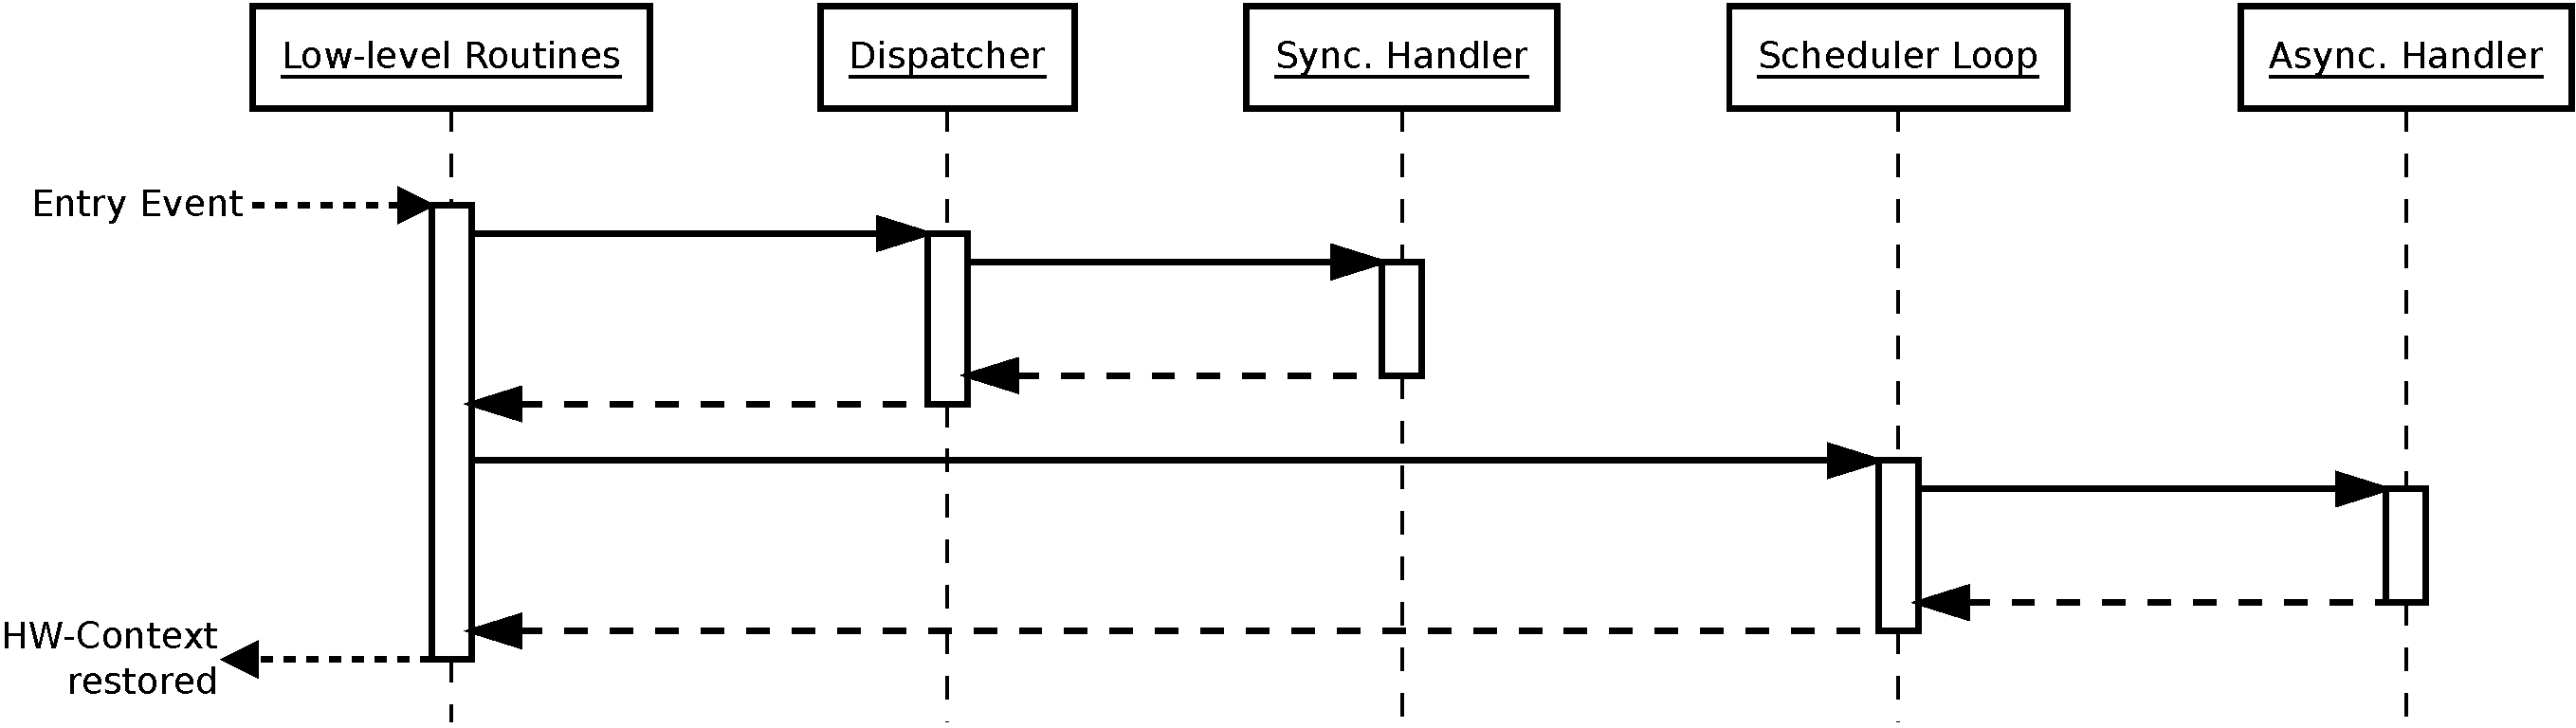
\includegraphics[scale=0.25]{fig/entry.pdf}
\caption{Kernel entry and exit sequence.}
\label{fig:kernel-entry}
\end{center}
\end{figure}

Both event types look very similar from the operating systems perspective. They both stop the execution of the user-thread currently running, start as synchronous events, and may schedule asynchronous event handlers. Figure \ref{fig:kernel-entry} illustrate the complete entry event handling from entering the kernel till exiting the kernel.

\begin{description}

\item[Kernel Entry Routine (sync):]
User-level interrupts automatically switch to a kernel stack and then store parts of the hardware context on the stack.
System calls are issued by a user thread and must to manually switch to the kernel stack and store the hardware context. Therefor, in contrast to interrupts and by convention, some parts (registers) of the hardware context are used for passing system call parameter, known to be volatile, or used to return a result value.

Both kernel entry routines save the hardware context and the entry reason into a context object pointed to by a hardware-thread-local variable. Typically, this object will be part of the current EC.
The kernel entry routines are \emph{synchronous}, implemented in \emph{assembler} and call a global dispatcher.

\item[Global Dispatcher (sync):]
For both event types, there is a global dispatcher that looks up a synchronous handler based on the \emph{interrupt number}, respectively \emph{system call number}.
The dispatcher then reads a reference to the current Execution Context from a hardware-thread-local variable and calls the handler, passing the Execution Context reference.

The global dispatchers is \emph{synchronous}, implemented in \emph{C++}, called by the kernel entry routine and calls a synchronous handler.

\item[Synchronous Handler (sync):]
The synchronous handler is the first thing that must know about the semantics of the event. It may decode parts of the hardware context in order to extract parameter or error codes, and selects what can be returned by a system call. The synchronous handler may call arbitrary synchronous methods or manipulate the stored hardware context in order to handle the event, but must not block.

If the handler requires to issue asynchronous calls in order schedule a an asynchronous handler, it must first acquire a Tasklet. There are two possibilities: either the event is related to the hardware thread (hardware exception or system call) or to a specific interrupt handler (async. interrupt).
In the first case, the handler can synchronously obtain a Tasklet from the current EC, which will be marked as blocked until the Tasklet is returned.
In the second case, the handler must own at least one Tasklet, and either masks its interrupt source or must accumulate additional interrupts until the Tasklet is return until a Tasklet is returned.

\item[Scheduling Loop (sync) / Asynchronous Handler (async):]
After the asynchronous handler returns, the dispatcher enters the task loop, that possible execute the asynchronous handler or other asynchronous tasks. The task executed may alter the state of the current execution context and its hardware context.
After all local tasks have been completed, the kernel returns into the kernel exit routine with the next runnable EC.

\item[Kernel Exit Routine (sync):]
The kernel exit routine does not depend on the entry event type of the last EC or next runnable EC. It simply restores the user-threads hardware context therefore exits the kernel.

The kernel exit routine is \emph{synchronous} and implemented in \emph{assembler}.

\end{description}


\paragraph{Discussion.}
\cite{DravesBershadRashidEtAl1991} introduces the Continuation model after discussing two different models:
The \emph{process model} have a separate kernel stack for each process.
% Thus, Creating a new Execution Context implies the allocation of new kernel stack.
The \emph{interrupt model} uses a single kernel stack for every entry into the kernel. When a thread would block in-kernel, it saves its whole contest, hence the stack.
In contrast, the \emph{continuation model} only stores a smaller context when resuming a system call.
% \cite{Warton2005} shows how the continuation model can improve the improve the performance of the L4 kernel.

As the event-based in-kernel programming model in seL4, OKL4 and Nova \cite{Heiser:2016:LML:2912578.2893177}, \mythos programming model only requires one stack per hardware thread. Logical control flow is represented by asynchronous object state and Tasklets, which enable \mythos to only store the processor state and the method of entering in order to resume a Execution Context later on.

\subsection{Boot Sequence}
\label{sec:boot-dyn}
% problem statement
The user-visible part of the system begins at the initial user thread, which usually is the first supervisor. In order to reach this point, it is necessary to initialise address spaces, start up the other hardware threads, create first kernel objects, and load the initial user thread.

% our solution
The boot sequence is performed in a sequence of stages that initialise subsequent layers of the kernel architecture.
%
\emph{Stage 0} is loaded and executed by the platform's boot loader or firmware in the raw physical address space. It creates an initial page table that contains the lower and higher half kernel codes at the correct logical addresses. Then, it switches to the x86-64 long mode and jumps to the higher half kernel code. 

The \emph{Stage 1} sets up the final kernel address space without the lower half kernel, because the lower half will be used as user space. This stage also sets up additional mappings as needed and configures sensible access rights. Its advantage over the previous stage is, that it can already use all of the kernel's code.

After switching to the final kernel address space, the \emph{Stage 2} is executed on the first hardware thread (aka Bootstrap Processor, BSP). It configures the root Untyped Memory object by setting the managed physical address range and inserting all free ranges that are backed by usable memory. For this purpose it can be necessary to parse the platform's memory table. The GDT, Core-Local Memory, Local APIC, and initial objects for all hardware threads are allocated from the root Untyped Memory. Finally, this stage uses the LAPIC to start up all other hardware threads and switches to the hardware threads actual kernel stack.

The \emph{Stage 3} is responsible for loading the initial user thread. This is part of the kernel as binary blob with a \texttt{text}, \texttt{bss}, and \texttt{data} segment with fixed logical addresses and limited size. A respective address space is created by allocating Page Maps, creating Frames out of the current physical position of the binary blob, and mapping these Frames at the predetermined logical addresses. The initial Capability Space is created by allocating Capability Maps and filling in all Scheduling Contexts (one per hardware thread), an initial Portal for system calls, the remaining Untyped Memory, and references to the own Execution Context, Address Space, and Capability Space. Then, the Execution Context's register set is initialised with the code entry point as instruction pointer and additional registers for the number of Scheduling Contexts and Untyped Memory objects. A user stack is not needed yet, because the supervisor can set the stack frames up on its own.     

\emph{Stage 4} is initiated by scheduling the initial user thread on the bootstrap hardware thread. All other hardware threads are still in their scheduling loop and wait. The initial user thread performs system calls through its Portal in order to configure its Address and Capability Spaces, create more Execution Contexts and so on. An initial communication channel to the external management service on the host computer is needed. This has to be provided by the Stage 3 setup. The implementation of this channel depends on the platform. Based on commands and data from this channel, the initial user thread loads applications and schedules them on the desired Scheduling Context.

% discussion and comparison
% TODO sigma0 in L4

%%%%%%%%%%%%%%%%%%%%%%%%%%%%%%%%%%%%%%%%%%%%%%%%%%%%%%%%%%%%%%%%%%%%%%
\section{Development View}
\label{sec:global-development-view}

This section describes implementation aspects, for example, the files and folders structure and the configuration management via code modules.

\subsection{Compile- and Run-Time Dependency Injection}
\label{sec:dependency-injection-impl}

% problem statement
Whenever objects or software components are created by instantiating classes, the question arises how the new objects will interact with the outside world. They require connections to other used services and usually also some context-dependent configuration. These dependencies can be fulfilled by queries to omnipresent directory services, by conventions, or via configuration methods and constructor arguments. 

% our solution
In order to simplify all aspects of instantiation, \mythos applies the principle of \emph{dependency injection} throughout all levels of the architecture and source code. This implies that no object or software component shall search on its own for its dependencies through global variables or omnipresent directory services. Instead, all dependencies and configuration is injected by the creator through constructor arguments and dedicated configuration methods.

This strategy separates the code responsible for instantiation and configuration from the
component's implementation. This helps to reduce the component's assumptions about its usage environment and protects against premature policy decisions.

\begin{description}
\item[Run-time value injection:]
During object creation, the creator passes pointers to used objects and configuration data by value via constructor arguments and additional configuration methods. This is the most commonly used form of dependency injection.

\item[Compile-time template injection:]
In C++, objects are created by instantiating classes and generic class definitions expose template arguments that need to be filled with actual type names and constants. This provides a mechanism for a template type based dependency injection. For example, in order to remove the overhead of virtual methods, the types of used objects can be injected alongside with the pointers to these used objects. This strategy is applied wherever type polymorphism is needed only for configuration but not during the actual execution. 

\item[Compile-time code injection:]
\marginnote{See also~\ref{sec:code-modules-impl}}
Some definitions and constants cannot be injected via template arguments and, sometimes, overuse of template arguments impedes the readability just a bit too much. In these situations, static code injection is applied by including generic header files that will provide the missing definitions. The build configuration management has to supply actual contents for these header files.
\end{description}


\subsection{Source Code Composition: Code Modules}
\label{sec:code-modules-impl}

% problem statement
Early work with \mythos showed that a single runtime-only configuration 
strategy is not sufficient. Some components
depend on specific hardware and compiler support, some performance
critical options require a static compile-time configuration.
At the same time, subtle differences between various platforms (xeonphi, quemu, bochs, gem5\ldots) and the desire to evaluate implementation variants required the ability to replace and recombine code fragments.

% our solution
% source files versus modules versus subsystems
\mythos avoids the conditional C preprocessor spaghetti by applying
the principle of dependency injection to the source code organisation.
Similar to grouping tightly related objects into components, related source files are grouped into \emph{modules}.
In this setting, the kernel objects of \mythos are the user-visible components and modules provide the class definitions that are needed to create the objects of these components. 

\begin{figure}
  \centering
  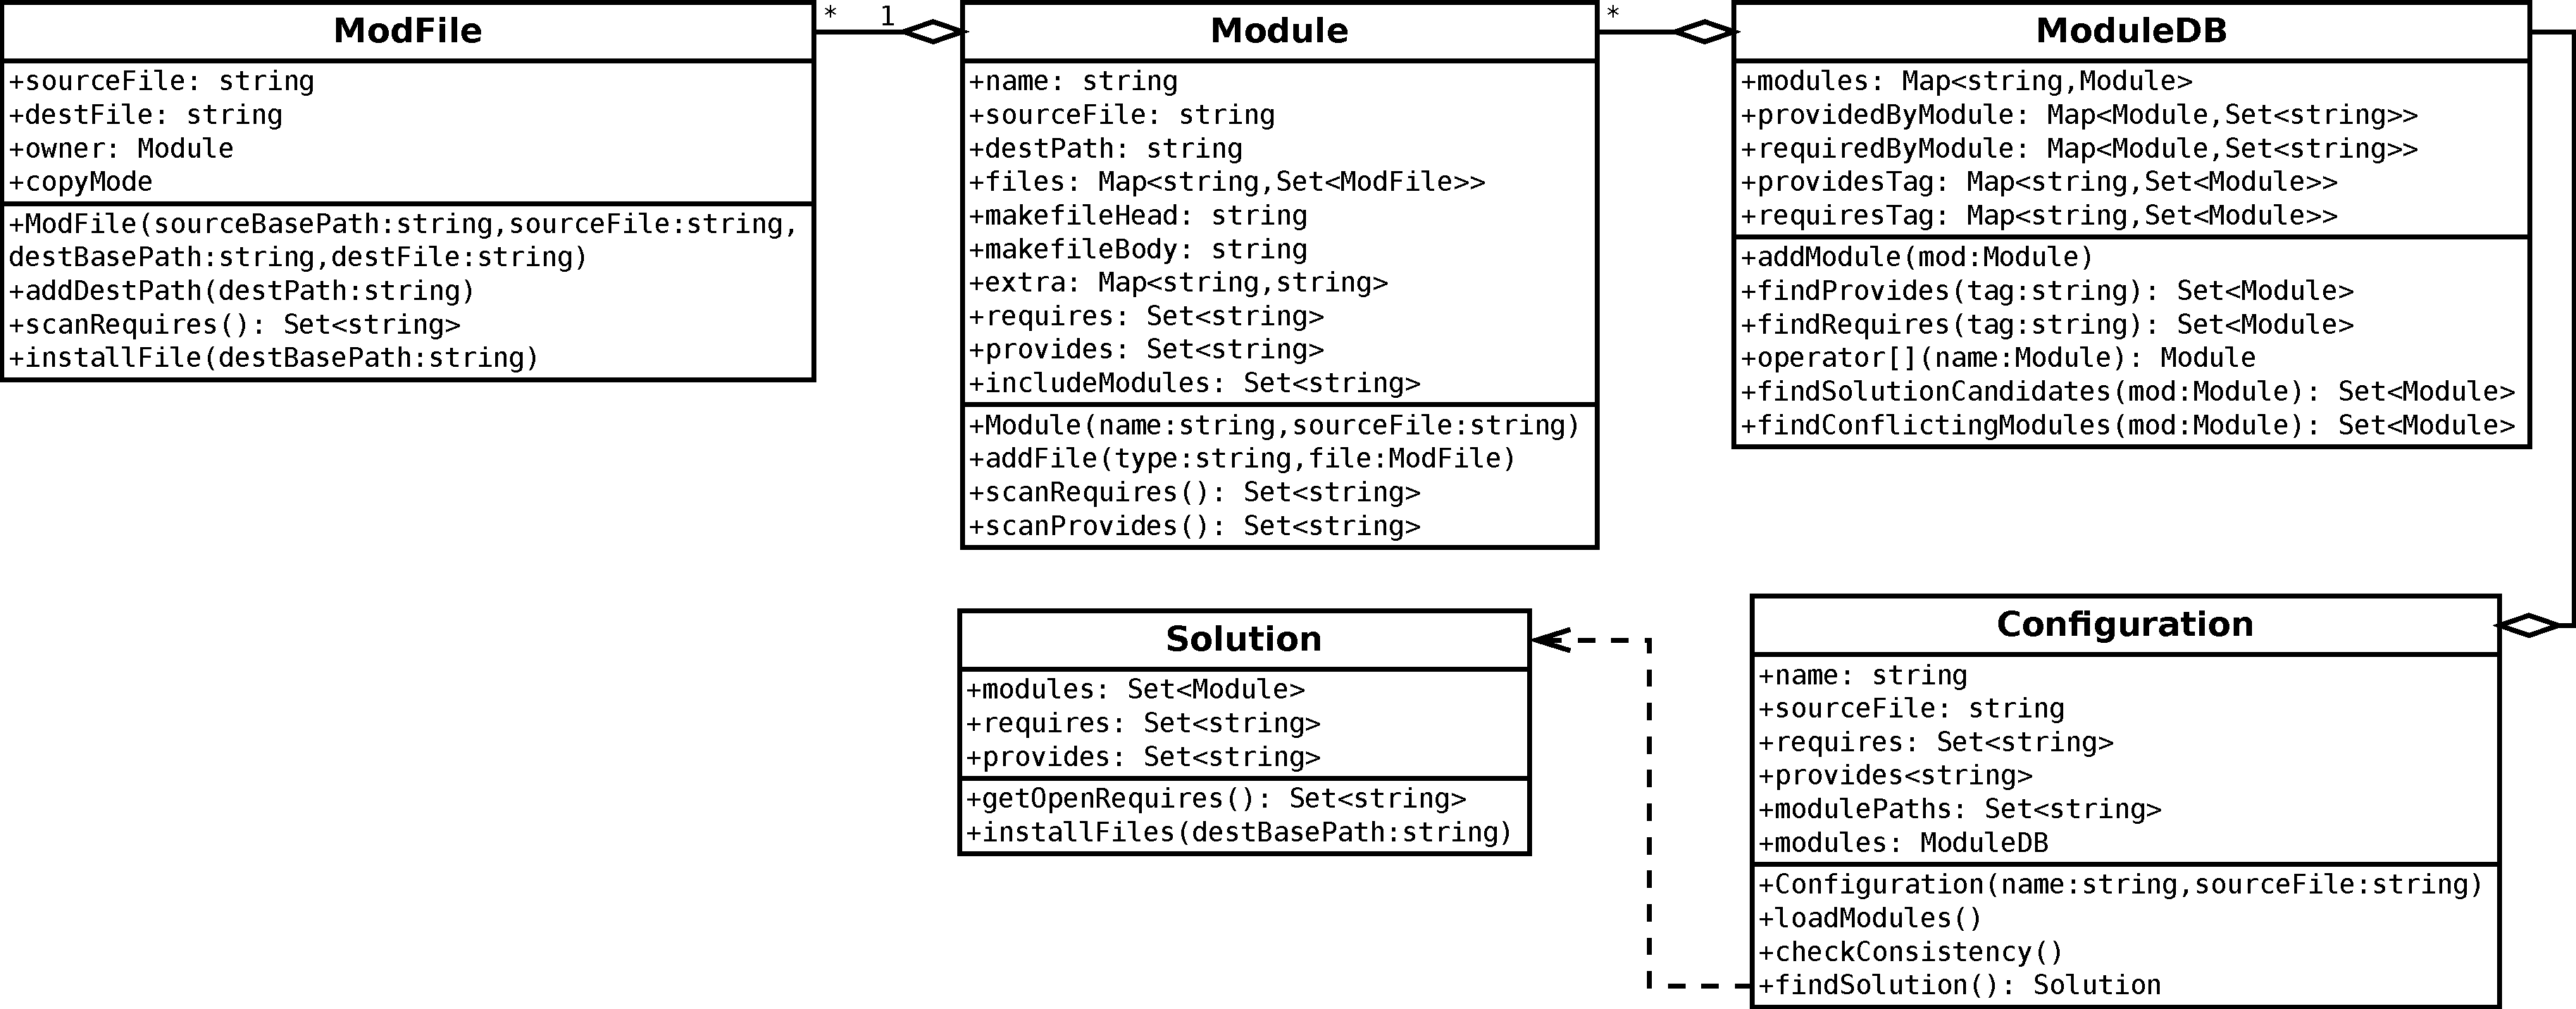
\includegraphics[scale=0.25]{fig/mcconf.pdf}
  \caption{Data model of the module and build target description.}
  \label{fig:mcconf-model}
\end{figure}

The build process is configured by the combination of \emph{module specifications} and a \emph{target specification}. Figure~\ref{fig:mcconf-model} gives an overview of the underlying data model. Basically, each module provides a set of source files and requires a set of files. For example, such dependencies can be header files with type definitions or source files with a specific implementation variant of a global function. Most dependencies are extracted automatically from the \texttt{\#include} directives in the provided source files. 

The target specification lists a set of requested modules or files. A simple resolution scheme is used to resolve dependencies: a list of missing files is collected from the requested modules and then additional modules are selected one by one if they provide one of the missing files. Two modules conflict when they provide files with the same destination name. In that case the dependency resolution reports an error and the developer has to manually select one of the possible modules by editing the target specification. In order to reduce the tedious work of selecting large groups of related module variants individually, the respective variants depend on a artificial \emph{tag} as resolution filter and the target specification provides this flag. For example, all modules that target the XeonPhi depend on \texttt{platform:knc} and all modules specific for the x86-64 architecture depend on \texttt{cpu:x86-64}.

\begin{lstlisting}[float, label=lst:module, caption=An example module specification.]
[module.boot-memory-multiboot]
  requires = ["platform:multiboot"]
  incfiles = ["boot/memory/Stage3Setup.h"]
  kernelfiles = ["boot/memory/Stage3Setup.cc", "boot/memory/Stage3Setup.cc", "boot/memory/Stage3Setup-multiboot.cc"]

[module.boot-memory-gem5]
  requires = ["platform:gem5"]
  incfiles = ["boot/memory/Stage3Setup.h"]
  kernelfiles = ["boot/memory/Stage3Setup.cc", "boot/memory/Stage3Setup.cc", "boot/memory/Stage3Setup-e820.cc"]

[module.boot-memory-knc]
  requires = ["platform:knc"]
  incfiles = ["boot/memory/Stage3Setup.h"]
  kernelfiles = ["boot/memory/Stage3Setup.cc", "boot/memory/Stage3Setup.cc", "boot/memory/Stage3Setup-sfi.cc", "boot/memory/Stage3Setup-knc.cc"]
\end{lstlisting}

Listing~\ref{lst:module} shows three example modules that provide the same header file \texttt{Stage3Setup.h} together with with different implementation source files. Instead of selecting one of the variants explicitly, build target specifications declare that they provide one of the platform tags, for example \texttt{platform:knc}. Then, just a single variant has all dependencies fulfilled and will be selected automatically to fulfil the boot codes dependency on \texttt{Stage3Setup.h}.

With respect to the layout of files and folders, modules are grouped into folders based on their respective subsystem with one sub-folder per module. These module folders contain a \texttt{modules.mcconf} file or several \texttt{.conf} files containing module specifications. The pathes to source files are relative to the position of the module specification. The target specifications contains a relative path to the root of the module folders.

The build process works as follows: given a target specification, the \texttt{mcconf} tool reads all module specifications, selects additional modules in order to fulfil open requirements, and then copies the references source files into the target folder. The configuration tool also generates a \texttt{Makefile} that contains rules for the compilation of the kernel source files and the linking of the final kernel image. Then, \texttt{make} can be used to compile and link the configured kernel. For this purpose, module specifications can contain Makefile fragments.

% TODO: Sometimes mcconf selects modules to solve other modules' dependencies and hits dead ends. The detailed log shows the reasons, e.g. needed header files. It would be nice if the command line output would directly tell these reasons as a kind of dependency backtrace. For this purpose, we have to record the reasons in each selected module during dependency resolution.

The top level source folder structure is roughly based on the horizontal layers. The folder name \texttt{tag} is reserved for \emph{tags}, a symbolic requirements do not refer to a file and is used to specify a configuration without the need to manually pick each platform-dependent module.

\begin{description}
\item[util] contains language level helpers and meta programming as well as logging facilities and generic data types.
\item[cpu] contains synchronous hardware abstractions.
\item[async] implements the runtime for asyncronous objects.
\item[objects] contains the implementation of concrete kernel objects and their runtime environment.
\item[boot] contains platform-dependent boot implementation, initializations and glue code.
\item[mythos] contains the interface  and definitions to be shared between kernel and user space.

\item[runtime] contains the user-space runtimen environment.
\item[lib] contains shared application code that is not part of the operating system.
\item[app] contains individual applications.
\end{description}

The modules folder structure mirrors the structure of the source folder. Each module lives in its own subfolder, shared code is extracted into modules with the suffix ``-common''. There is an additional \emph{build} folder that contains modules facilitating the build process, for example by adding appropriate compiler flags to the makefile.

\paragraph{Discussion.}
% C++ objects versus components versus kernel objects
A \emph{software component} is a C++ object or a group of C++ objects that work
tightly together to provide a specific service and that share the same life cycle.
Although less relevant for \mythos, components should be designed with substitute-ability, reusability, and composition in mind. 
The difference between arbitrary language-level C++ objects and components are the more restricted rules governing the component's interfaces, life cycle, and interactions. Language-level objects are used to implement components but also to implement data structures, containers, communication channels, function objects, messages and so on.

The seL4 kernel uses some clever Makefile constructs in order to copy the platform- and process-specific files into the right place. Dependency injection is applied by including header files at generic locations, for example \texttt{arch/types.h}, that are not actually present in the source code. The actual files are created during the build process by generators or by copying specific implementations, for example \texttt{arch/x86/types.h}. 
%
The Fiasco.OC kernel uses a mix of a custom C++ preprocessor and the Linux kernel's preprocessor-based configuration tool. 

\subsection{Interacting Asynchronous Objects via Tasklets}
\label{sec:tasklet-impl}

\epigraph{It has therefore recently been suggested that one should combine a shared variable and the possible operations on it in a single, syntactic construct called a monitor. It is, however, too early to speculate about what this approach may lead to.}{Per Brinch Hansen: Concurrent Programming Concepts, 1973.}

% problem statement
The asynchronous objects' responsibility is to implement delayed and delegated execution as base mechanism for the kernel's concurrency and locality control. Main challenges for any asynchronous execution are the encoding and decoding of the desired action into messages, the storage and transfer of these messages, and the storage of the dynamic processing state.     

% our solution

\begin{lstlisting}[float, label=lst:async-object, caption=An example asynchronous object.]
class Adder {
public:
  void add(Tasklet* msg, AdderResponses* res, int a, int b) {
    monitor.exclusive(msg, [=](Tasklet* msg){this->addImpl(msg,res,a,b);} );
  }

private:
  MutexMonitor monitor;

  void addImpl(Tasklet* msg, AdderResponses* res, int a, int b) {
    // do something ... then respond
    res->addResult(msg, a+b);
    monitor.release();
  }
};
\end{lstlisting}

Listing~\ref{lst:async-object} shows an example implementation of an asynchronous object. The \texttt{Adder} provides the asynchronous method \texttt{Adder::add()} that allows two add two integer numbers.
Given a Tasklet \texttt{msg}, a pointer \texttt{a} to an Adder instance, and a pointer \texttt{r} to a matching response handler object, the asynchronous method is called with \lstinline|a->add(&msg, r, 1000, 1)|. In line 4, the call and its arguments are captured into a C++11 anonymous function (aka closure, lambda expression) and passed to the Adder's monitor (line 4). The monitor uses the passed Tasklet to schedule the delayed and possibly remote execution of the anonymous function. The actual implementation \lstinline|Adder::addImpl()| in line 10 performs its work and, then in line 12, calls one of the result handler's methods, passing along the Tasklet for the asynchronous execution of the handler method. In line 13, the monitor is informed, that the request processing has finished. This is necessary for the asynchronous object deletion. \marginnote{See also~\ref{sec:async-deletion-dyn}}

All execution is non-blocking and, hence, waiting synchronously for results of calls to asynchronous methods is not possible---and not necessary. Instead, \emph{request} methods also retrieve a reference to a response object that acts as continuation and sink for the result data. Such \emph{response} methods consume the tasklet and results as arguments but have no argument pointing to another response handler.

\begin{figure}
  \centering
  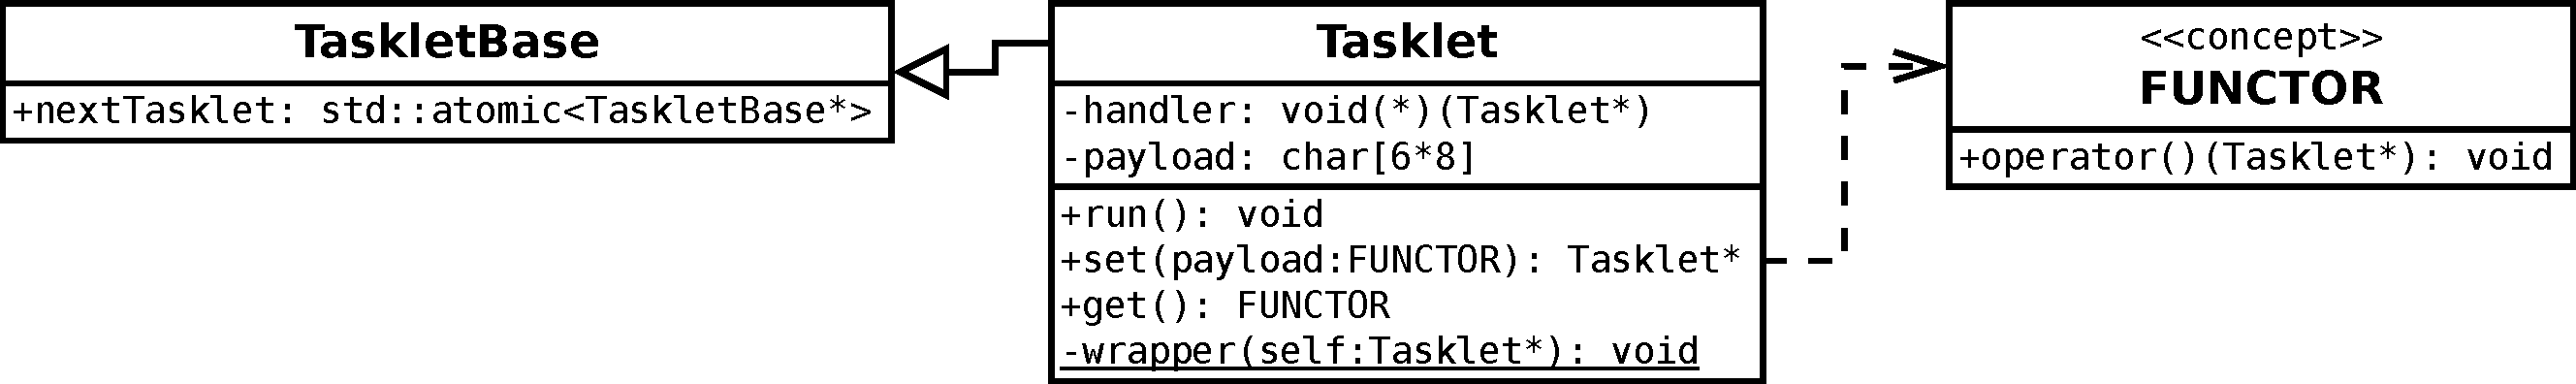
\includegraphics[scale=0.25]{fig/tasklet-class.pdf}
  \caption{Class diagramm of the Tasklet implementation.}
  \label{fig:tasklet-class}
\end{figure}

Figure~\ref{fig:tasklet-class} shows the Tasklet's class diagram. The base class contains an C++11 atomic variable that is used by monitor implementations to manage task queues without dynamic memory management. The pointer is in a separate base class in order to simplify the usage of small dummy objects for the queue management. 

The Tasklet class itself contains a C function pointer very similar to \emph{active messages}. This handler function is responsible for executing the actual function object that was stored through the \lstinline|set()| method in the payload. Instead of the function pointer, a virtual method could have been used. This would consume the same space but adds a second memory lookup via the vtable pointer. The Tasklet implementation contains a generic static implementation for these handler functions.

The size of the payload is chosen such that Tasklets are exactly one x86-64 cacheline large (64 byte). This leaves four 64-bit words for direct call arguments. Any additional arguments have to be passed via a pointer to an argument structure, which is provided by the caller.

\paragraph{Discussion.}
Often, user threads or coroutines are used to store the dynamic processing state. These are based on a separate stack for each of the currently active executions. The separate stacks allow to suspend and resume the current execution at arbitrary points by switching between stacks. While very convenient, a major drawback is the need to reserve a sufficient amount of large enough stack in advance. Suspending an execution usually requires to switch to a new coroutine or thread in order to be able to begin the next pending execution. This again requires dynamic memory management.

Message passing as a middleware layer tends to hide the allocation and deallocation of message buffers in order to increase the conceived convenience. This introduces a hidden dynamic memory management and adds considerable send and receive overhead. The \mythos design avoid both by using Tasklets as caller-provided message buffers and, hence, can be used with no or very simple caller-internal allocation mechanisms. 

Decoding retrieved request and response messages involves figuring out what should be done with the message and, then, to unpack the attached payload into usable, correctly typed arguments. A method call dispatcher would interpret a logical identifier in order to choose which code to execute. This usually introduces multiple conditional branches into the execution path. Instead, Tasklets as active messages use a single unconditional jump. 

Encoding and decoding the arguments requires a client and a server stub code. The publicly visible asynchronous method fulfills the role of the client stub and the anonymous function acts as server stub. The use of C++11 lambda expressions shifts the tedious work of argument encoding and decoding into the C++ compiler. This exploits that the caller and callee code is compiled by the same compiler and resides in the same kernel image.

\subsection{Managing the Resource Inheritance Tree}
\label{sec:capability-impl}

% problem statement
Storing the complete resource inheritance tree can be very space consuming and most of the information is never used. This reduces the system's efficiency through increased cache and TLB trashing and complicates the concurrent update operations on the inheritance tree. In addition, not all possible inheritance operations have a well-defined meaning. For example, what should happen with the children when a capability that has derived children is copied? Who is responsible for the object deletion when the root capability of an object is copied?

% our solution
\mythos uses a set of rules to restrict the types of capabilities that may be derived to create children and which may be copied to create siblings in the inheritance tree. The basic idea is to maintain a strict \emph{contained-in} relation between the kernel objects and their children. For example, a Portal that was allocated from an Untyped Memory is contained within the address range of the Untyped Memory.

Now, just \emph{references} to kernel objects require separate handling because they represent the same address range as the capability they were derived from. The basic idea is to use a flag in the capability in order to mark it as weak reference. This allows to revoke all references and inform the affected capability subject or object.

However, supervisors may want to transfer access capabilities, which are weak references too, to other applications and retain the option to revoke these individually. For example, a different clients retrieve Portal references to the same portal. In order to keep the different clients apart, these references do not inherit from the original portal but from an intermediate \emph{derived} capability. 
Thus, two flags in the capability are used to represent \emph{original}, \emph{reference}, \emph{derived}, and \emph{reference to derived}. 

\begin{figure}
  \centering
  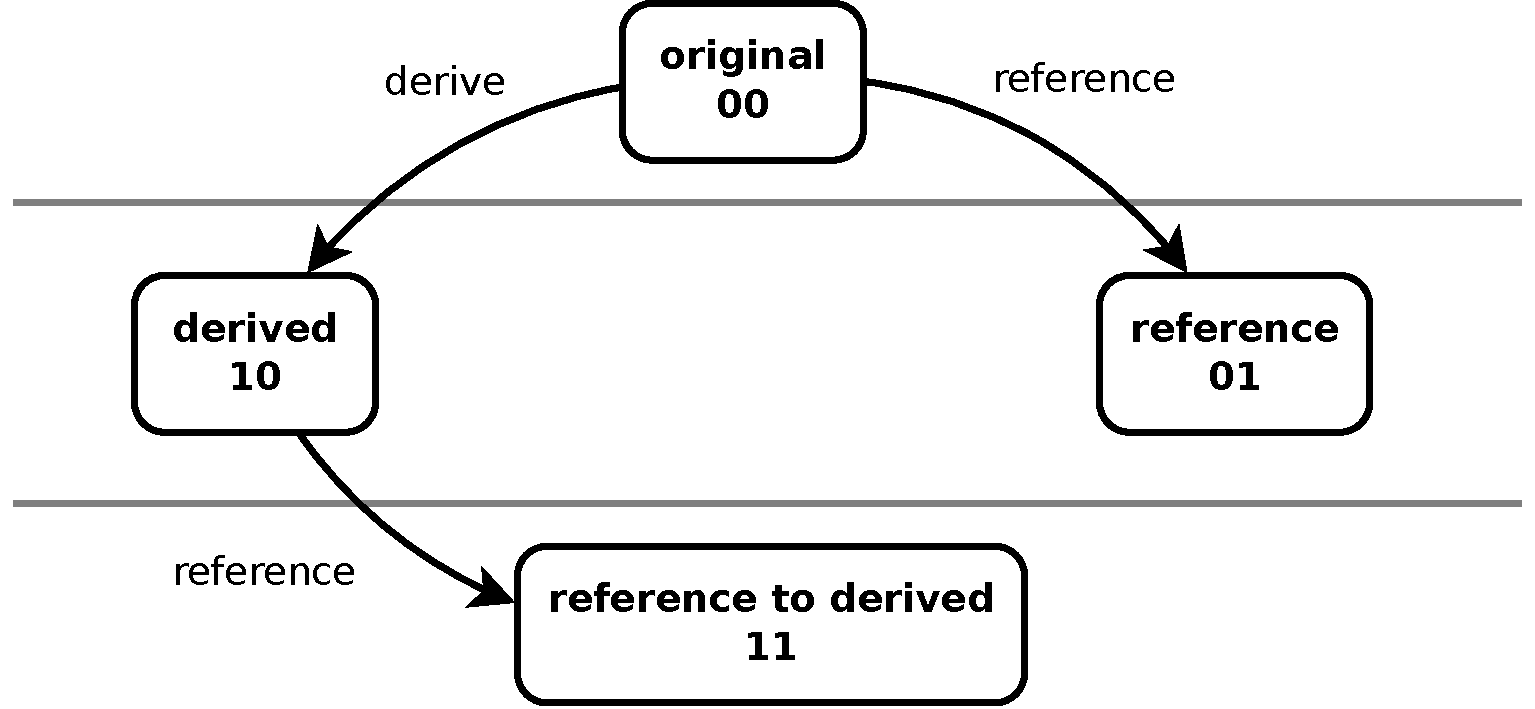
\includegraphics[scale=0.25]{fig/DerivedReferenceBits.pdf}
  \caption{Derivation and reference capability flags. References to derived capabilities can be revoked without revoking other derived capabilities and references to the parent.}
  \label{fig:cap-types}
\end{figure}

This derivation and reference scheme is illustrated in Figure \ref{fig:cap-types}. For example, the original capability can point to a Portal. A reference to the original enables the holder to operate on the Portal as if owns the original. The actual access rights can be restricted through the reference's meta-data. The derived capability of the Portal can be used to hand out derived references to a client application. These can be revoked by revoking the derived capability.  

The same rules are required to differentiate Frames, mapped Frames, derived Frames, and mapped derived Frames. The mapped frames are weak references and are mainly used by the Page Maps to track the usage dependencies between address spaces and frames. The derived frames are used to hand out the right to map frames without loosing the ability to revoke just these mappings.

The above rules have following implications: inheritance from a capability creates a child if the new capability is (a) a reference to an original capability, (b) a reference to a derived capability, (c) a derivation from an original capability, or (d) an original capability that is a real subset of the parent original capability. 
Inheritance creates a sibling in the tree if the new capability is (e) a reference created from a reference, (f) a derivation created from a derivation, or (g) an original capability that has the same address range as its parent capability.
All other cases are prohibited and the rights management may further restrict the inheritance.
% \mythos does not allow the case (g) in order to reduce the amount of reference counting in kernel objects.

\begin{figure}
  \centering
  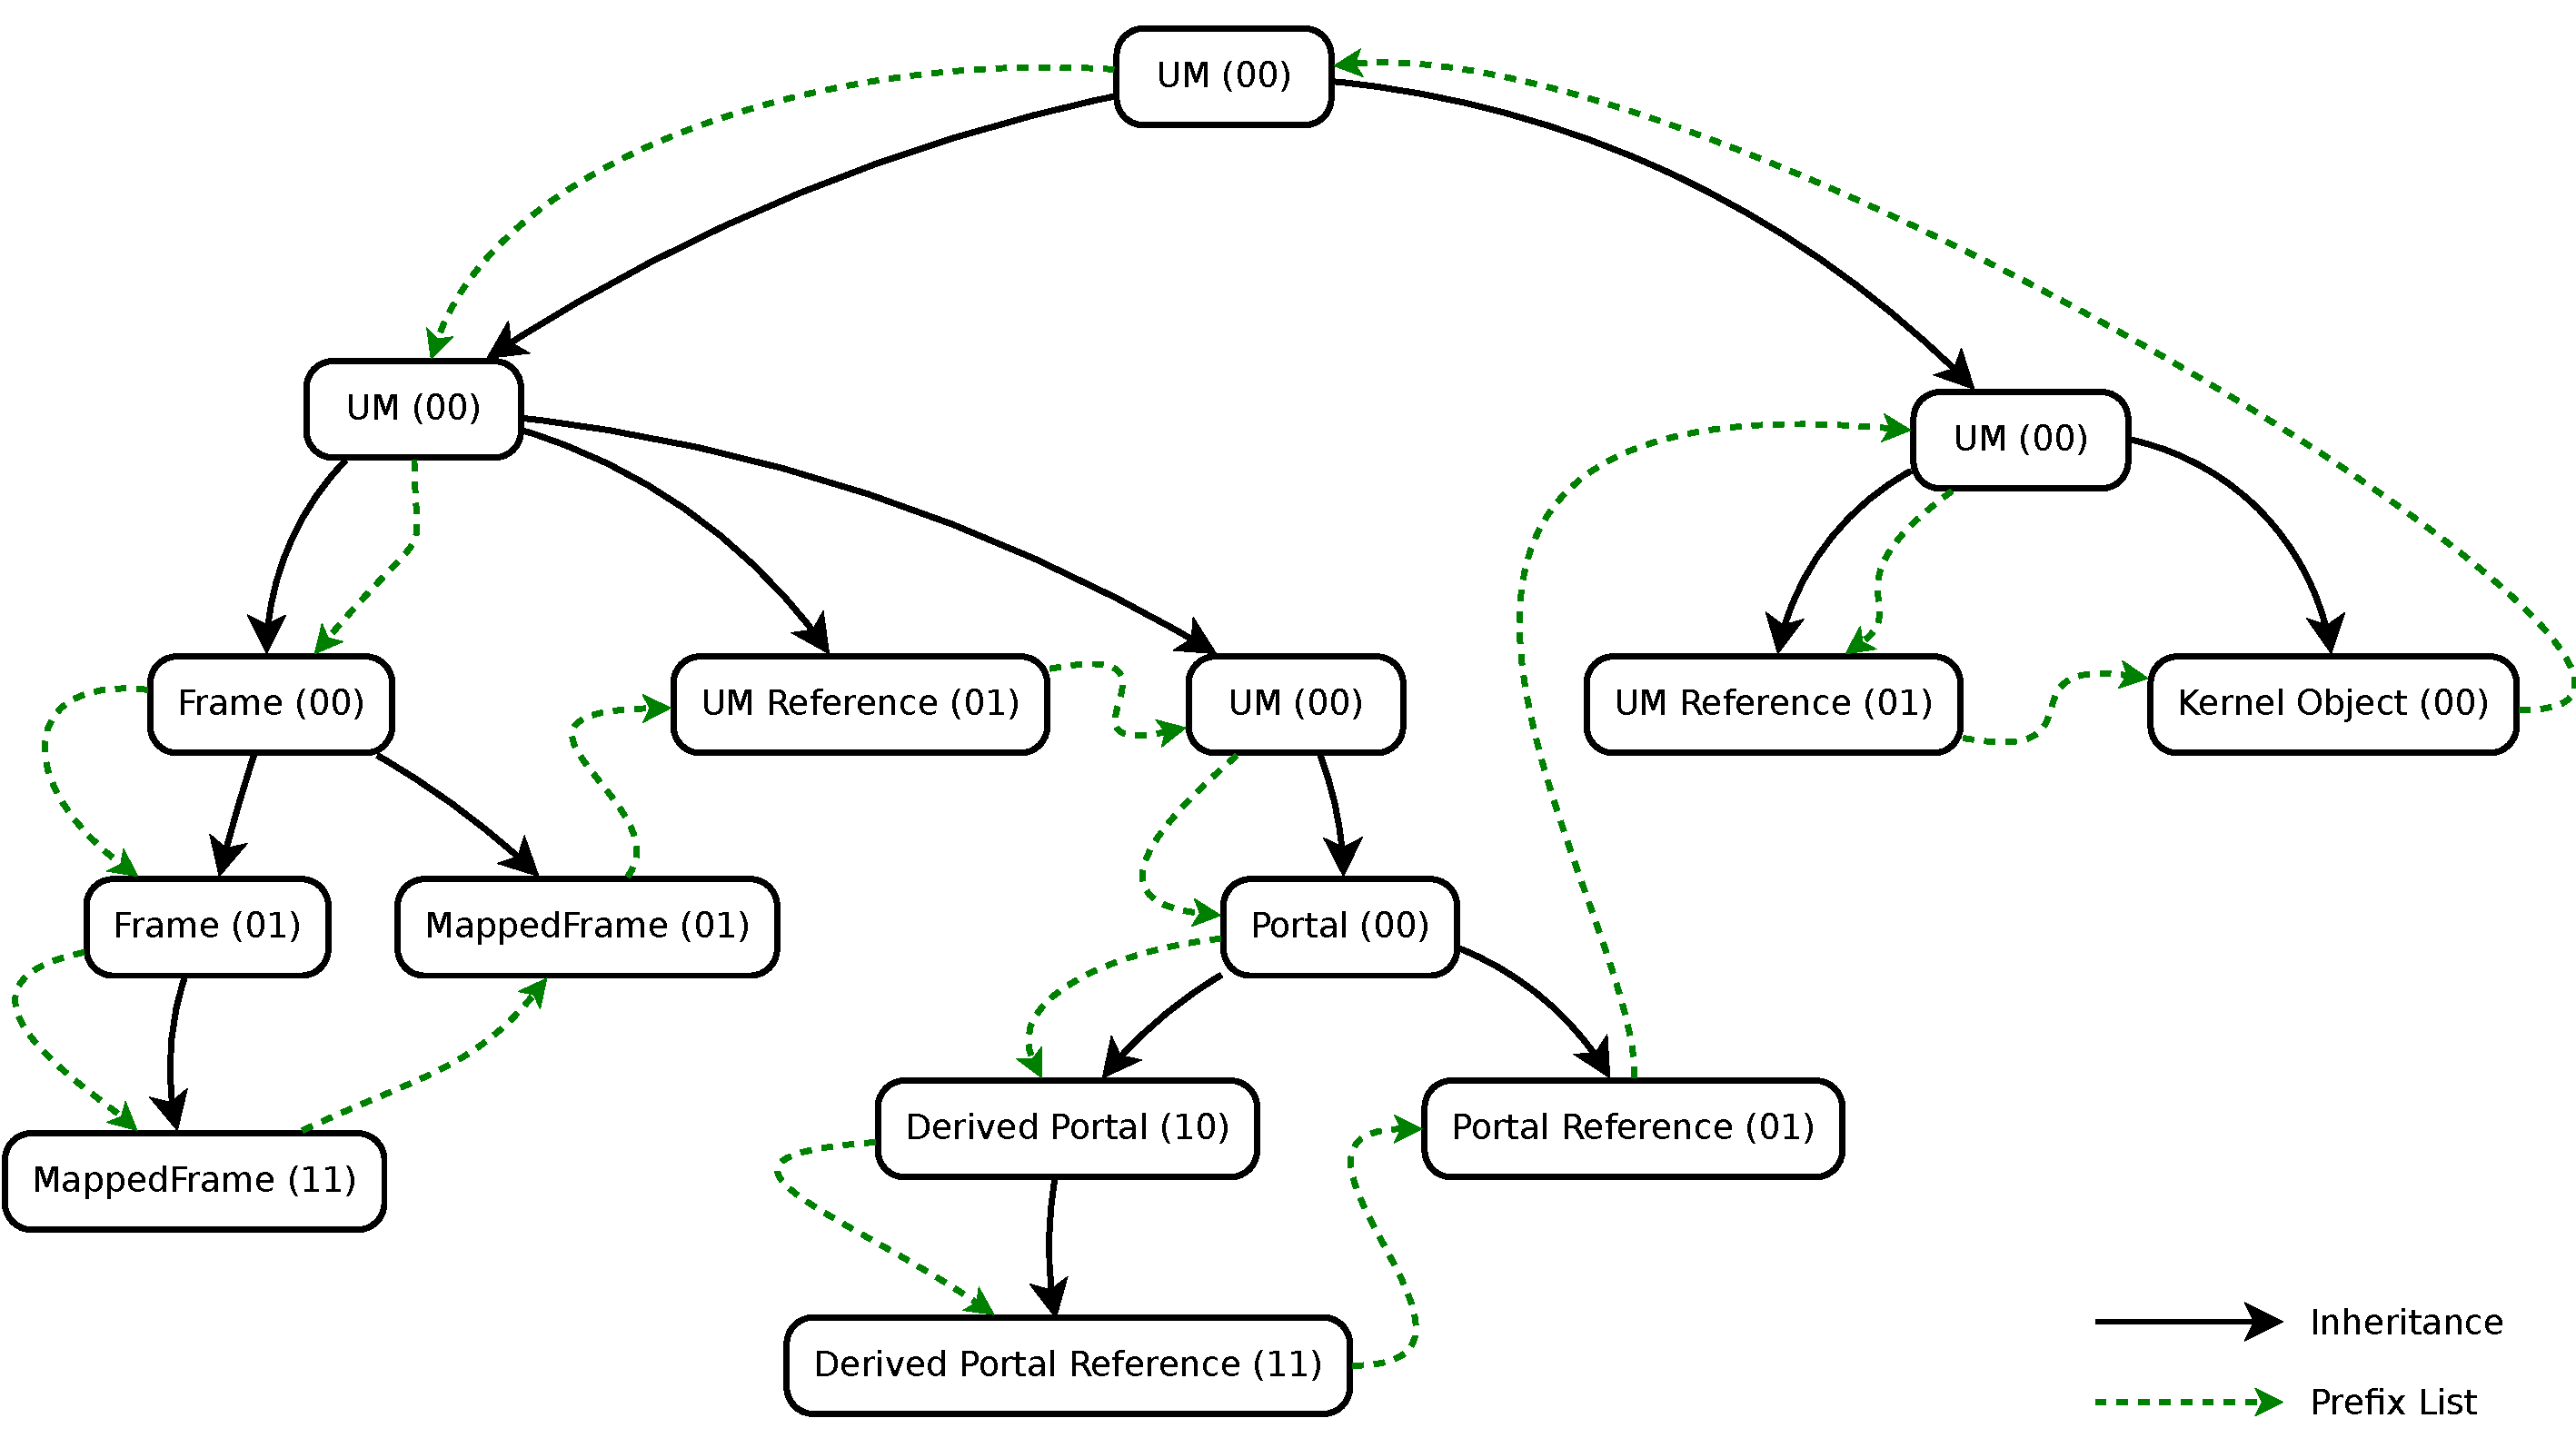
\includegraphics[scale=0.25]{fig/cap-tree.pdf}
  \caption{An example resource inheritance tree. UM is Untyped Memory. The two digits mark original, derivation and reference capabilities. The dotted arrow shows the actually stored prefix serialisation.}
  \label{fig:kernel-object-cap}
\end{figure}

In combination, this allows to store just the \emph{prefix serialisation} of the inheritance tree in a double linked circular list. Figure~\ref{fig:kernel-object-cap} gives an example. The root of the tree is the initial Untyped Memory object that represents all of the kernel's usable memory and is statically owned by the kernel. The circular list avoids to deal with the special case of the list's end. Children are inserted directly behind the parent into this chain. In order to insert a sibling behind a capability, it would be necessary to skip all existing children. Instead, a sibling is inserted before the capability that it inherited from, which equally ensures that both stay within their parent's subtree.

The parent-child relation is not stored explicitly because the objects and properties of the capabilities are sufficient to decide this relation. This is just needed for the revocation of access rights and deletion of kernel objects. By construction, all children are directly behind the parent in the chain. The subtree ends when reaching a capability that cannot be a child of the subtree's root. This \emph{is-child-of} test is successful if (a) the address range owned by the child is a real subset of the parent's range, or their ranges are equal and (b) only the child has the reference flag, or (c) only the child has the derived flag.

\begin{figure}
  \centering
  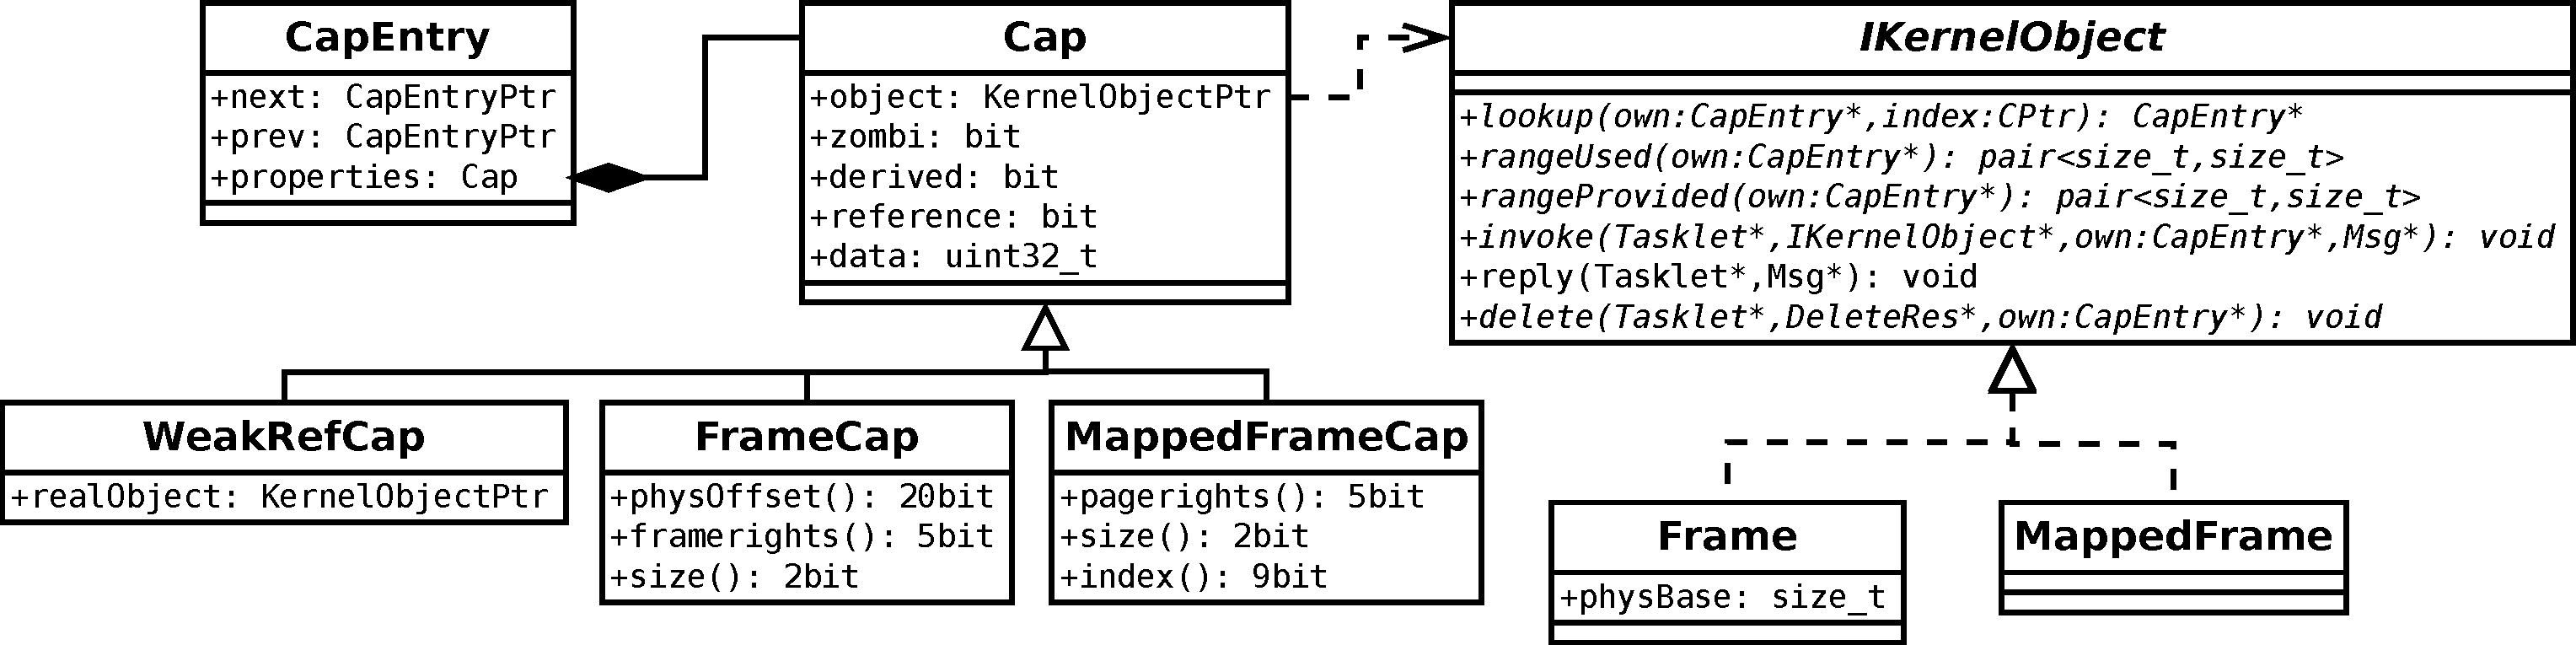
\includegraphics[scale=0.25]{fig/kernel-object-cap.pdf}
  \caption{Class diagram of the prefix-serialised resource inheritance tree.}
  \label{fig:kernel-object-cap}
\end{figure}

Figure~\ref{fig:kernel-object-cap} shows the class diagram of the inheritance tree. The capability entries \texttt{CapEntry} store the double-linked chain and the meta data \texttt{Cap}. The meta data is designed to fit into a 64-bit register. The first 32 bit contain a compressed pointer to the kernel object that is the capability's object. The capability's subject, that is, the holder of the capability entry is not stored by default. The kernel object has to provide the actual information for the inheritance tree management. Most important are \texttt{rangeUsed} and \texttt{rangeProvided} for the \emph{is-child-of} test. The second 32 bit contain arbitrary type-specific meta-data that is processed only by the kernel object. For this purpose, a pointer to the capability entry is passed to all respective methods.

Because of the limited size of the kernel space and the 8-byte alignment of all objects, pointers can be represented with just 29 bits. The remaining three bits are used for status flags such as zombi, derived, and reference. Frames store a 4KiB aligned offset into a 4GiB address window, which requires just 20 bits. The base address of the window is stored in the Frame object.

Weak reference capabilities, for example mapped frames in a page map, require additional consideration. On revocation, the \texttt{delete()} method of the capability's object pointer is called in order to inform the affected kernel object. If this points to the original referenced object, a weak-reference flag and a pointer to the actual subject (the reference holder) is needed in the meta-data. In many cases, it is easier to replace the capability object by a helper kernel object that is part of the subject and knows how to clean up the revoked reference. For example, the object of \texttt{MappedFrameCap} points to a respective kernel object that is part of a \texttt{PageMap}. This leaves more space for other meta-data.

\paragraph{Discussion.}
The idea of using the prefix serialisation of the inheritance tree was inherited from seL4's implementation. They differentiate between capabilities on untyped memory, \emph{original} capabilities that can only be derived from, and \emph{derived capabilities} that can only be copied~\cite{GrosvenorWalker2016}.
Unlike our presented solution, their \emph{is-child-of} test inspects the types of the capabilities and applies type-specific rules. Our solution requires just a call to a virtual method in order to query the type-specific address range calculation and everything else is independent of the kernel objects.

Ideally, it would suffice to compare the managed address range of the parent against the used address range of the child only if both are original capabilities. In most cases, the reference and derivation capabilities that follow in the chain have to be children. Unfortunately, the Untyped Memory nodes in the inheritance tree can contain original capabilities as well as own references and derivatives. Hence, the range comparison is mandatory. We do not optimise away this comparison because it is used just during revocation, which is not expected to be fast anyway.

\subsection{Operation Implementation in the Inheritance Tree}
\label{sec:capability-ops} 

Even given the structure of the Inheritance Tree, described in Section \ref{sec:capability-impl}, and the approach to safely delete individual objects, described in Section \ref{sec:async-deletion-dyn}, it is non-trivial to implement high-level operations on Capability considering these operation might be executed parallely.

There are three major categories of operations to consider: The \emph{read operations} read a capability in order to create a reference or call a asynchronous method. The \emph{local operations} locally update the Inheritance Tree, like \emph{derive}, \emph{reference}, but also \emph{moving} a capability into another entry.
The \emph{global operations} consists of operations that may delete whole subtrees of the Inheritance Tree, such as \emph{delete} and \emph{revoke}.

There are several race conditions between operations from different or the same category. The value of a Capability is only updated atomically, and can be marked as a zombie to prevent reader from using the value. A simple solution to resolve the races between writers is protecting the whole Inheritance Tree with a global mutex. However, this serializes all operations which manipulate capabilities.

\begin{figure}
  \centering
  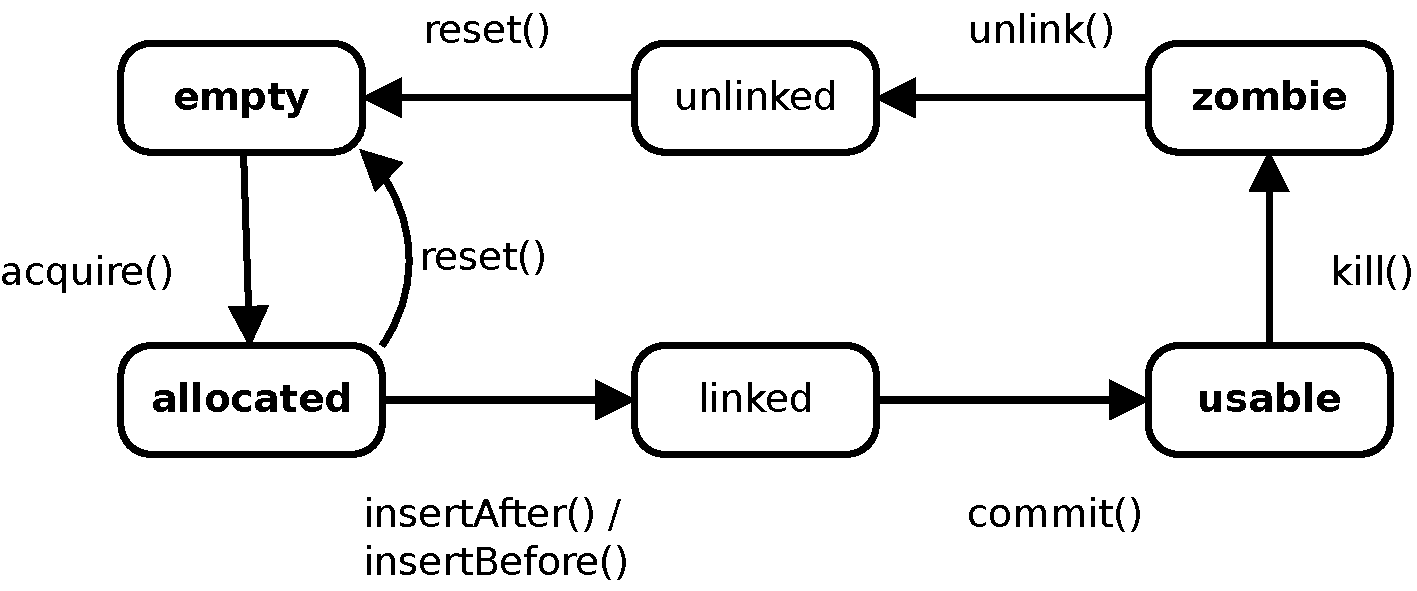
\includegraphics[scale=0.25]{fig/capability-states.pdf}
  \caption{States of the capability object and related operations. State visible from observing only in the capability value are bold.}
  \label{fig:cap-states}
\end{figure}

In order to implement a finer grained locking, individual entries in the inheritance tree (CapEntries) must provide a lock. Similar to the \emph{overhand locking} technique, entries must lock itself and the previous entry in order to be removed. When travesing the list, the lock on the previous entry is release before acquiring the lock on the next entry.

Independant from the locking process, every capability entry has additional states that describe its lifetime cycle, and are illustrated in Figure~\ref{fig:cap-states}:

\begin{description}
\item[empty] In this state, the Capability entry is not linked into the Inheritance Tree, contains no pointer to an object, and has no additional flags set. Such an entry can only be \emph{allocated}.
\item[allocated] After being allocated, the is claimed to be used to store a capability. After allocating the slot, a can try to acquire furter resources, e.g. memory. If that fails, the entry is \emph{reset} into the \emph{empty} state.
\item[linked] This state is the same as the allocated state, but the entry is linked into the tree. After it has been linked, it must be \emph{commited} before the current control flow suspends.
\item[usable] The usable state is the only state in which a subject can access the object through the capability. A usable capability always contains the pointer to a invokable Kernel Object.
\item[zombie] This is a state where the capability still contains the pointer to an kernel object. This enable to revoke the right to access an object immidiately.
\item[unlinked] This state is the same as the zombie state, but the entry is removed from the tree. Unlinking the entry can be used as a sequencer in order to determine who will delete the object.
\end{description}

\paragraph{Read operations} just load the capability value atomically and check whether the capability is usable, before the pointer value is used to either create a counted reference or issue a request to the object. Races between these requests and delete operations are resolved by the protocol described in Section \ref{sec:async-deletion-dyn}.

\paragraph{Local operations} manipulate the Inheritance Tree locally and synchronously, thus the can hold locks during the their execution. However, to avoid race conditions with long-running global operations, these local operations must inspect the state of the capability entry and abort if a race is detected. For example, a zombie capability can not be derived nor moved. In order to facilitaty the implementation of the global operations, certain entries can also be pinned to prevent their capabilities from being moved.

\paragraph{Global operations} potentionally manipulate large portions of the Inheritance Tree and potentionally run for a long time. In order to prevent long-term active waiting, global operations only lock the entrys they are currently manipulating. Races with read or local operations are resolved by setting approbiate flags, such as the zombie flag of the capability or the pinning flag of the entry. Global operation must also take special care to synchronize with each other.


\subsection{Delete and Revoke Operation}

Delete and Revoke are both global operations that potentially manipulate large portions of the Inheritance Tree and can lead to the deletion of objects. This section presents some of the difficulties encountered and the solution implemented. The main difference between the revoke and the delete operation is that revoke does not require the deletion of the capability the operation is started on. Here, this capability is called the operation's \emph{root capability}, which is not to be confused with the root capability of the Inheritance Tree.

\paragraph{Problems}

\begin{itemize}
\item working with ranges (esp. revoke)
\item concurrent deletion on subtrees
\item cap entries in kernel objects
\item deleting objects deletes itself
\item deletion order in a single deletion object
\end{itemize}

\paragraph{Solution}

A synchronous delete function that can be called recursivly. The function is only allowed to be called by the deletion servive or a the synchronous revoke capability handler of a kernel object.

\begin{enumerate}
\item starting from the root capability, scan throught all children and mark them as zombie.
\item starting from the root capability, do a depth first search in order to find leaf capabilities and revoke them.
\item If a original capability is revoked, add the object to the deletion list, then call delete recursively on every entry contained in the object.
\end{enumerate}

After the synchronous phase has terminated, the deletion service issues the deletion broadcast and then asynchronously deletes the objects on the list in a FIFO order. Each call to the delete function first inserts all child capabilities in a leaf-to-root order and, after that, deletes entries in the object to be deleted. Therefore, the complete list is in a leaf-to-root order, as object inserted to the list after another object are either unrelated or higher in the Inheritance Tree. In conclusion, these objects will be deleted in the correct order.

\subsection{Invocation Buffer}
\label{sec:invocation-format}

The invocation buffer is 512 byte buffer in a Frame created from Untyped Memory. Therefor it is read-  and writeable  by the kernel using direct mapped memory. The overall invocation process is not concerned with the semantics of the Invocation Buffer. However, Capability Transfer demands to distinguish Capability Pointers from plain binary data. On the other hand, Invocations on Kernel Objects require a calling, respectively, marshaling convention\marginnote{See also~\ref{sec:invocation-handling}}. Table \ref{tab:invocation-format} shows how the Portal operations interact with the Invocation Buffer.\marginnote{See also~\ref{sec:portal-dyn}}

\begin{description}

\item[Message Tag]
The message tag (32bit) consists of a Label, the message length, the number of referenced capabilities and a mask.

%{\centering
\begin{bytefield}{32}
\bitheader[endianness=big]{0-31} \\
\bitbox{16}{\tiny Label} &
\bitbox{7}{\tiny Message Length} &
\bitbox{3}{\tiny Extra Caps} &
\bitbox{6}{\tiny Unwrapped Mask}
\end{bytefield}
%}

The \emph{Label} (16bit) is not interpreted by the message transfer. Invocations to kernel objects use this value as message descriptor similar to a system call number. The response message stores the error code in the Label.
%
The \emph{Message Length} (7bit) holds the length of the message as number of 4-byte words. It is used to copy less data in small messages. The message's receiver usually can infer the payload size from the message's label. 
%
The \emph{Extra Capability} (3bit) field holds values from 0 to 6 and describes how many capability are transferred in the cap.\ array.
%
The \emph{Unwrapped Mask} (6bit) determines which capabilities from the extra cap.\ array shall be unwrapped (in) and which capabilities have been unwrapped (out).

\item[Message] The message is a oblique byte array with a size of 480 bytes. Its is not interpreted by message transfers. Invocations to kernel objects will read arguments from this here and write results into this field.

\item[Capability Pointer Array]
The Capability Pointer Array consists of 7 entries (32bit, 4bytes), with the first entry being reserved. When sending a messages (\texttt{invoke}), the dest.\ capability points to the slot in the invoker's capability space where the response capability transfer should put the transferred capability. When receiving a message (\texttt{wait}), the dest.\ capability field contains the badge of the portal capability that was used as message target by the sender. When sending a reply, this field points to the capability in the repliers's capability space that should be transferred back as reference capability.

%\item[Capabilities Space]
%This is a reference to a Capability Space the addresses in the Capability Pointer Array are relative to.

\end{description}

\begin{table}
\begin{tabular}{lr|ccccc}
\toprule
field & size & invoke & invoke+wait & listen & listen+wait & reply  \\
 & & (in) & (out) & (in) & (out) & (out) \\
\midrule
msg. tag & 4B \\
~~label & & request & response & ignored & request & response \\
~~msg. length & & req. len. & res. len. &  480 & req. len. & res. len.\\
~~extra cap. & & request & response &  & request & response \\
~~unw. mask. & &  &  &  &  &  \\
\midrule
msg. buf. & 480B & request & response & - & request & response \\
\midrule
cap. array [0..6] & 7*4B \\
~~dest. cap [0] & & transf. dst. & - & - & badge & transf. cap. \\
~~extra cap [1..6] & & request & response & - & request & response \\
\bottomrule
\end{tabular}
\caption{Invocation Buffer Format. op+wait denotes either for a wait or a successful pull operation after a operation. }
\label{tab:invocation-format}
\end{table}

\paragraph{Discussion}
The format of the Message Buffer and Message Tag format is heavily inspired by seL4 IPC IPC buffer data structures~\cite{GrosvenorWalker2016}.
However, the number of extra capabilities has been increased in order to reflect the needs of factory method calls.

seL4 implements Capability Transfers between user-threads.
This is especially useful for capability exchange between applications that do not have supervisor-supervised relationship.
However, the current application requirements for \mythos do not demand for such an mechanism. Therefore, it will not be implemented in the current iteration. Supervisors have control over the supervised Capability Space and can therefor use numeric identifiers to manually lookup and create Capabilities on the appropriate positions.

seL4 furthermore unwraps capability badges of capabilities that reference the invocation target. This enables supervisors to store internal identifiers directly in the supervised Capability Space. The reduce the need to track the content of the supervised Capability Space in the supervisor.

\mythos might implement Capability Transfer and Capability Unwrapping in later iterations, as it promises to simplify the implementation of supervisors for complex programs. Therefore, the Unwrapped Mask in the Message Tag is reserved. For the supervisors required by the compute cloud scenario, Capability Spaces are expected to by simple enough to be managed without further support.


\subsection{Invocation Handling}
\label{sec:invocation-handling}

In Section \ref{sec:invocation-format}, the low-level format of an invocation message and a simple marshaling convention has been presented. In contrast, this section illustrates by examples how Kernel Obects handle invocations and how concurrent application runtimes may expose the invocation to the programmer.

\paragraph{Invocation Handling in Kernel Objects}

Listing \ref{lst:inv_skel} illustrates invocation handling in the kernel: \emph{invoke} is a ordinary asynchronous function and part of every the Kernel Objects interface. It multiplexes between \emph{different protocols} and invokable \emph{methods} using the \emph{protocol identifier} and \emph{method identifier} introduced in Section~\ref{sec:invocation-format}. As most Kernel Objects, the example object only support a single protocol. After the concrete method has been identified, the monitor is requested to execute the implementation of the method. When a method or protocol is requested that is not implemented by the Kernel Object, it immediately returns calls the response handler with a error code.

In the implementation of the invoked method, the invocation message is interpreted further to extract the arguments.
Moreover, the capability is inspected to check if the caller is allowed to invoke the function. If anything fails, the appropriate response \marginnote{See also~\ref{sec:portal-dyn}} is issued. Otherwise, the actual work is done and the context of the invocation is used to return a response according to the protocol. As required for every asynchronous method, the implementation must signal the completion of the request to the monitor.

\begin{lstlisting}[float, label=lst:inv_skel, caption=Kernel-side dispatch and implementation of a method invocation.]
void Adder::invoke(Tasklet* t, InvocationCtx* ctx, CapEntry* cap) {
  switch (ctx->protocol()) {
  case ADDERPROT:
    switch (ctx->method()) {
      case ADD: 
        monitor.request(t, [=](Tasklet*t){this->add(t,ctx,cap)} );
        return;
      }
    break;
  }
  ctx->response(t, CORE, UNKNOWN_METHOD);
}

void Adder::add(Tasklet* t, InvocationCtx* ctx, CapEntry* cap) {
  int a, b;
  bool success = ctx->readMsg(a,b);
  if (!success || !AdderCap(cap).canAdd()) {
  	ctx->response(t, CORE, success ? DENIED : INVALID_MSG); 
  	monitor.requestDone();
  	return;
  }
  // work with ctx->thread(), cap, a, b ...
  ctx->response(t, ADDERPROT, SUM, a+b);
  monitor.requestDone();
}
\end{lstlisting}

\paragraph{Invocations in Application Runtime Environments}

Application runtime environments are expected to provide a concurrent programming model, such as coroutines or events. Listing \ref{lst:inv_stub} illustrates how asynchronous invocations can be integrated into an environment which facilitates deferred synchronous execution with \emph{futures}: The invocation is wrapped into a deferred synchronous function that stores its result into a future. Depending on the application-side programming model, the future may trigger an event or reschedule a coroutine when the invocation is completed. Therefore, the application-level idle loop waits for \emph{any} invocation to complete and uses the \emph{user context} \marginnote{See also~\ref{sec:portal-dyn}} in order to dispatch the appropriate response handler. User-level server or services can be implemented analogously: Listening on a Portal also is a deferred synchronous method that returns when a request arrives.

\begin{lstlisting}[float, label=lst:inv_stub, caption=Example for issuing invocation user-side.]
void Adder::add(Portal* p, Future f, int , int b) {
  p->invoke(this->obj, ADDERPROT, ADD, f, a, b); 
}

// ... in app's idle loop:
Portal* res = wait();
if (res) res->handleResponse(); // pushes results to f
\end{lstlisting}


\paragraph{Marshaling Conventions}

Per convention, all invocation messages where the most significant bit in the first byte of the message is set are in the kernel invocation format.

In the message, Capabilities should referenced by there offset in the Capability Index Field.

\subsection{System Calls}
\label{sec:system-calls-impl}

% TODO which calls? which parameters? in which registers? invocation message structure?


Invocations are implemented on top of implementation level system calls, which modify the state of \emph{Portals}. The semantic of these calls is described in Section \ref{sec:portal-dyn}.

\subsection{Error Detection and Handling}
\label{sec:error-handling}

% problem
Errors in a operation system can have multiple causes: incorrect usage of system call, hardware faults and programming errors.
Almost every operation systems must be resilient against misuse of system calls and programming errors, which are converted into \emph{logical exceptions} when detected, and may lead to \emph{hardware exceptions} if not detected or not handled properly. \emph{Hardware faults} can either lead to \emph{hardware exceptions}, e.g. ECC fault, or to \emph{interrupts}.

% solution
\emph{Hardware exceptions} occur synchronously when processing a certain instruction. Typical examples are Page and Protection Faults, and Invalid Instruction Exceptions.
As such, hardware exceptions can be attributed to the asynchronous object currently being run and incorporated into a error handling scheme as described for logical errors. However, currently this is not the case. \emph{Interrupts} occur asynchronously and can not be attributed to a concrete object or control flow. As such they are best handled by the normal interrupt handling procedure.
Finally, \emph{logical exceptions} are handle error discovered by the normal control flow. Triggering logical exceptions often is an appropriate mean to prevent hardware exceptions: for example, checking for a null pointer might prevent a page fault exception. The rest of the section focuses on the propagation and handling of logical errors.

After a exception is raised, it must be propagated to an appropriate handler. In \mythos, we differentiate between two different dimensions: \emph{horizontal} error propagation between \emph{asynchronous and kernel objects}, and \emph{vertical} error propagation in the \emph{synchronous control flow}.  The next paragraphs describe the error propagation in on the different \emph{vertical layers}\marginnote{See also~\ref{sec:vert-layer}}, as illustrated in Figure \ref{fig:error-propagation}.

\begin{figure}
  \centering
  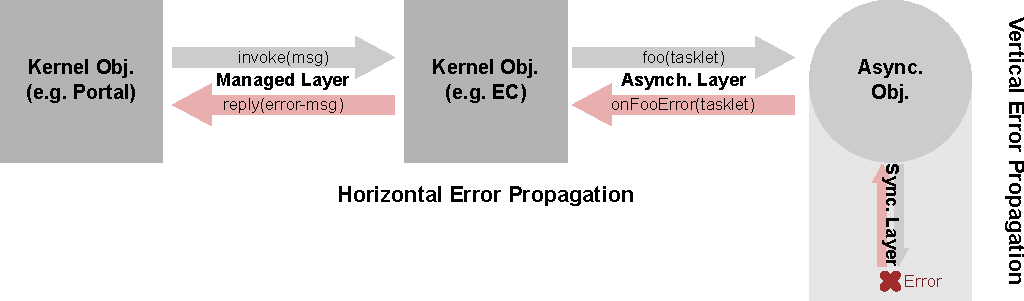
\includegraphics[width=\textwidth]{fig/error-propagation.pdf}
  \caption{Vertical and horizontal error propagation across different layers.}
  \label{fig:error-propagation}
\end{figure}

\paragraph{Synchronous Error Propagation:}
In a \emph{synchronous} control flow, errors are propagated \emph{vertically} up in the stack. In the  current \mythos implementation, \emph{vertical error propagation} is implemented via return values with the \lstinline$optional$ type. A function returning a optional value can either return \emph{a concrete value} or an \emph{error code and no value}. This is different from, e.g., returning a null pointer, which is in itself a possible value and does not allow returning a error code. When required, this mechanism might be switched out for another vertical error propagation mechanism, for example \emph{C++ language level exceptions}.

\paragraph{Error Propagation between Async. Objects:}
If the error can not be handled in the current synchronous control flow, it must be propagated \emph{horizontally} between \emph{asynchronous objects}. 
\emph{Horizontal error propagation} is implemented by exploiting the \emph{client/server pattern} \marginnote{See also~\ref{sec:concurrency_control}} between asynchronous objects. Instead of calling the \emph{response handler} of the client, the server responds by calling an separate \emph{error handler}. This separates all handling of non-synchronous errors into the error handler, freeing the response handler from verbose error checking. Hence, all errors are propagated to the client.
The error handler can then decide whether it can handle the error, for example by retrying, or propagates the error even further. An asynchronous object might enter an \emph{error state} where it replies to all pending and incoming requests through a designated error handler, unrelated to the semantic of the request. This mechanism might be used in order to isolate objects in which a hardware exception has occurred.

\paragraph{Error Propagation between Kernel Objects:}\todo{this paragraph depends much on the invocation process}
On a higher layer, hence the \emph{Managed Layer}, error still must be propagated horizontally between different objects. However, in the managed layer, only communication through messages is possible. Here, the error is propagated via an error message in a well-defined format.\todo{See also~\ref{invokationformat}}

As \emph{invocation} also is the main communication mechanism between the \emph{application layer} and kernel objects, this is the way how errors are propagated back to the user.
Typically, kernel objects perform a first sanity check on the \emph{invocation request message} before starting to carry out the request and potentially delegating sub-tasks as asynchronous calls.

\paragraph{Error Handling in the Application Layer:}
\hspace{0em}\marginnote{See also~\ref{sec:error-dyn}}
An application must assume that, potentially, every invocation will return a error message. Application level services might implement sophisticated strategies such as \emph{supervisor trees} \cite{Armstrong2003} in order to systematically handle errors.
On the other hand, \emph{hardware exceptions} and \emph{lookup faults} in the Capability Space are translated into invocations to a \emph{exception handler kernel object} which is determined by the \emph{Execution Context}.

\paragraph{Discussion.}
Choices OS implements a wide variety of error detection and correction methods \cite{DavidCampbell2007}:
Code Reloading recovers corrupted code sections, whereas Component Micro-Reboot can recover from corrupted data structures.
In the mindset of microkernels, \emph{restartable system components} and their corresponding \emph{supervisors} are canonically implemented outside of the kernel. In-kernel code is expected to be correct, whether proven by verification or assumed after intensive review of the small kernel code base. On the other hand, this does not prevent kernel code and data structures from being corrupted from hardware fault. Choices OS implements restartable components in user-mode.% and a supervisor/watchdog in kernel?
On the error detection side, Choices OS implements \emph{in-kernel C++ exceptions} as a general error handling mechanism, and transforms processor exceptions into language level exceptions.

\subsection{Image-based Debugging Facilities}
\label{sec:core-dump}

% problem

% solution
Because the system memory in \mythos is only 4GiB large, it feasible to create an image of the whole system memory by using DMA from the host. Host accesses to the coprocessor memory are cache-coherent if the host-side caching is disabled.

Although it is possible create a kernel image without further kernel support, concurrent changes to the kernel memory can easily lead to an inconsistent image.
\mythos supports two different methods of obtaining a consistent kernel image: \emph{Snapshot Images} capture a consistence state by issuing a non-maskable interrupt (NMI), which dumps the processor state into the stack, and waiting \emph{in the interrupt handler} until the image is captured. In contrast, a \emph{Checkpoint Image} is created by using a interrupt to force all threads into the kernel, but instead of waiting in the interrupt handler,  all threads wait \emph{before the next Monitor or Execution Context is dispatched}. This allows to create an kernel image that is easier to analyse, since there are no ``non-commited transactions'' of asynchronous object monitors.

%\paragraph{Discussion.}

% TODO: TempMemoryAccess mit host-spezifischen IPhysMemoryMapper

% TODO: Infrastructure for Systematic Testing

%\chapter{Kernel-Level Scheduling and Concurrency Control}
\label{chapter:kernel-scheduling}



\chapter{Extensions for x86-64 and Intel XeonPhi KNC}

\begin{description}
\item[Control Channel:]
At least the first user-mode supervisor requires a communication channel to external tools on the host processor. \mythos does not aim to be a self-sufficient kernel and the control channel is the only initial interface from the user into the running system. Depending on the target platform, different implementations are needed, for example via PCIe shared memory on the XeonPhi versus a virtual serial IO port on emulators. Control Channels behave similar to Portals as communication endpoints and badged reference capabilities can be used to multiplex virtual channels. 
\item[Debug Channel:] this kernel object provides a simple interface to the kernel's internal debug and trace messages subsystem. It is needed to see what the first supervisor does. Additional channels can be set up and configured by the supervisor.
\end{description}

The channel kernel objects could be replaced by platform-specific code in the supervisor. However, the initial channel via shared memory has to be at a fixed physical address in order to simplify the connection initiation. Channels via IO ports requires additional kernel support to enable io port access for the user-mode supervisor. Both would require additional kernel code while increasing the supervisor's complexity. Therefore, we choose to use custom platform-specific kernel objects for this purpose.


%%% -------------------------------------------------------------------
\section{Short Messages over PCIe2}
\label{sec:short-message-channel-pci}

% problem
The communication between host services, such as the application launcher and
the \mythos services on the many-core accelerators, is carried out via
asynchronous message passing over PCIe2. As already explained, a similar
mechanism can be established between different \mythos instances or components
hosted on different processors, which are backed by shared memory. In this
particular case, the majority of messages relates to control and configuration
akin to remote method invocations or remote system calls. These require just
small messages with a size limit in the order of a few cache lines.

Data transfers may need larger messages. One way to implement them, is splitting
the transfer into multiple small messages, which does not need additional
services. In the long term, dedicated mechanisms for large data transfers, for
example via DMA engines, can be added. These would be coordinated through short
messages.

% requirements
Separate message channels are needed for each direction, that is from host to
accelerator and from accelerator to host. On the producer site, support for
multiple concurrent producers is desirable. This ensures, that all threads can
send messages without the need for locking based mutual access or forwarding to
a proxy thread. On the consumer side, such support for concurrent access is not
strictly necessary. A main thread would be responsible to pull new messages and
convert them into local tasks. A single consumer queue can be combined with a
non-blocking mutual exclusion mechanism to hand over the work to an idle thread.

The PCIe 2.0 network allows to map the accelerator's physical memory into the
logical address space of applications running on the host processor. The host
service can directly write and read the accelerator's memory almost like normal
shared memory. However, careful protocol design is necessary because the PCIe
2.0 network does not keep the caches coherent, atomic operations like
fetch-and-add are not supported, and the involved processors may have a
different view on the logical and physical address spaces.

The interaction across multiple address spaces implies the need for memory
pinning. The host operating system and \mythos must be instructed to never
migrate the frames that contain the communication channel data. Otherwise,
processors will read from and write to wrong positions, which are not observed
by their counterparts. The easiest way to achieve this is by placing all shared
communication data on the \mythos side. There we, know the physical address of
the channel and can ensure that the data will not be moved. For shared data on
the host side, which runs a Linux system for example, two steps are needed:
First, the allocated pages have to be pinned in order to prevent migration and,
second, their physical addresses have to be provided to the \mythos side. These
need to be translated then into accelerator-physical addresses in order to
become accessible from \mythos.

\subsection{Logical View: Slotted Circular Buffer}

Using a fixed size memory area is the easiest approach for host to accelerator
communication because just this area needs to be mapped into the logical address
spaces once. Hence, a slotted circular buffer design was chosen: The messages
are stored in a fixed size array with slots of fixed size (a few cache lines).
The producer and consumer sides use independent counters for their logical read
and write positions. The actual positions are modulo the number of buffer slots.
Each slot contains a state header for flow control between producers and
consumers. The producer writes sequentially into different slots of the circular
buffer while the consumer tries to catch-up the producer counter. The flow
control information is provided for each slot and it is used to establish an
access protocol between the producer and the consumer, which will be explained
later in this chapter.

The unidirectional channel is split into three data structures:
ProducerSide, ConsumerSide, and ChannelData. This allows to place the respective
parts into the appropriate memory, which enables the local use of atomic
operations. Just the ChannelData is in the shared memory, which restricts it to
ordinary read/write access and C++11 atomic load and store operations.

The ProducerSide and ConsumerSide objects contain the respective logical
read/write positions and a pointer to the the ChannelData according to the local
logical address space. No access to the other end's state is needed.

\subsection{Physical View: Consumer vs. Producer Side}

For host to accelerator direction, the ProducerSide is placed in host memory
while ConsumerSide and ChannelData are placed in the accelerator's memory. For
the reverse direction, the ProducerSide and ChannelData are placed in the
accelerator's memory and the ConsumerSide is placed in the host memory.

The host has the ChannelData mapped with CacheDisabled and
WriteCombining flags. The write combining makes sending more
efficient. Ideally, the incoming channel's data should be mapped with
caching enabled. 
% TODO: what is the benefit of that, since incoming data will change 
% throughout the communication process? 
Unfortunately, the currently used driver interface
does not support this mode.

\subsection{Dynamic View: Cache Control}

Initially, the producer and consumer side logical positions are zero. The slot
headers are initialized accordingly to be recognized as ``free''.

A producer acquires a logical write position by atomically incrementing a local
write counter. This supports concurrent producers. A producer then polls the
header of a respective slot until the slot is marked ``free'' (by being equal to
the acquired logical position). Then, the message data is written into the slot
and, finally, the slot is marked as ``occupied'' by setting a respective bit.

The consumer polls the slot of its current logical read position. If the slot is
marked as ``occupied'', the data is copied or processed directly. Then, the
consumer writes the slot's next logical position into the header in order to
mark it as free and selects the next responsible producer at the same time.
Finally, the consumer has to invalidate the slot from its L1 and L2 caches and
increment the logical read position.

Access to shared memory over PCIe is not cache coherent. Reads to remote memory
can be cached in the local cache, but writes to this memory will not invalidate
these replica. Hence, the memory has to be mapped in \texttt{Cache Disabled}
mode or the communication protocol has to implement proper manual cache line
evictions. Usually, writes over PCIe should invalidate the destination's caches
automatically. Unfortunately, currently this does not seem to work for writes
from host to XeonPhi. Hence, the \texttt{CLEVICT0} and \texttt{CLEVICT1}
instructions were used for manual cache line evictions.

The \texttt{CLFLUSH} and \texttt{MFENCE} instructions are not available on the
XeonPhi. The new \texttt{CLEVICTx} instructions evict the requested cache line
from the local L1 or respectively L2 cache but do not broadcast the evict
request to other caches. Hence, all threads that read from \texttt{ChannelData}
have to evict their data before reading the next message.

\emph{Future: Concurrent consumer support is possible by using a second bit in
the slot header to mark the slot as locked by a consumer. This is done with an
atomic compare-and-swap such that just a single consumer can succeed. All other
consumers proceed to the next slots. Unfortunately, compare-and-swap is
available only on the side that has the \texttt{ChannelData} in its local
memory.}

\subsection{Development View}

Because the cache invalidation works differently on host and XeonPhi, two
different implementations of the of the producer and consumer sides of the
circular buffer are needed. These versions can be also be adapted more easily to
specific needs of the respective the side. In our current implementation
\texttt{ProducerSide} is specialized in the classes
\texttt{PCIeRingProducerX86} (for the host) and \texttt{PCIeRingProducerPhi}
(for the \mythos side). Both extend a generic interface \texttt{ISendChannel}.
Likewise, a \texttt{ConsumerSide} is implemented in the classes
\texttt{PCIeRingConsumerX86} and \texttt{PCIeRingConsumerPhi}. Both extend the
interface \texttt{IRecvChannel}.

The basic interface provided by \texttt{ISendChannel} has the methods
\texttt{acquireSend()} and \texttt{trySend()}. The acquire method returns the
logical write position, which is then handed to the send method.
\texttt{trySend()} has to be repeated for the provided position until it
succeeds. This non-blocking interface allows higher software levels to intermix
polling for incoming messages.
  
The basic interface provided by \texttt{IRecvChannel} contains the methods
\texttt{hasMessages()}, \texttt{tryRead()}, and \texttt{finishRead()}. The first
method can be used to check whether there is a pending message without trying to
read or write anything. \texttt{tryRead()} returns a pointer to message data and
might lock an appropriate slot for concurrent consumer support. After a message
has been processed, its address is provided to \texttt{finishRead()}, which
flushes the respective caches and marks the slot as free.

\emph{Implementation Note: The \texttt{ChannelData} structure is generic and has
a slot type attribute as well as a slot count attribute. The slot type is
combined with the channels slot header to define the actual slots and slot size.
In consequence, the ProducerSide and ConsumerSide classes get the actual
ChannelData type as template type argument.}

%%% -------------------------------------------------------------------
\section{Textual Debug and Binary Trace Output}
\label{sec:debug-channel}

\mythos components produce a configurable amount of textual debug and log
messages via the \texttt{mlog} subsystem.  The \texttt{mlog} subsystem is
integrated within all mythos modules and provides user interfaces for creating,
filtering and sending log messages to customizable log sinks. One such sink is
for example the debug output channel to the host. Currently the system is
configured to send all levels of debug information of all subsystems over the
PCIe2 channel to the host, where it can be further processed, e.g. stored into a
file or printed on a terminal console. A per-module configuration of a
debug-level is realizable as well.

Textual messages have a variable unbounded length and should be able to contain
multi-line messages. Besides this, all hardware threads can produce messages
concurrently and their output should be sequentialized for better readability
(a multiple producers channel). Writing messages to a single output channel can
be a blocking operation, because the communication is just one-way and, thus, no
deadlocks are possible. Performance is not important because production systems
would disable almost all debugging outputs.

In order to reduce the implementation effort and potential for errors,
the short message channel from Section~\ref{sec:short-message-channel-pci} is
reused. Just a more specific message format had to be defined.

\todo{this might belong into the more general dev view}
Several different \texttt{mlog} channels for different subsystems, e.g. memory management and userspace, are provided.
Additional channels can easily be added. Each channel can output messages of different priority levels, as indicated by the programmer, which can be filtered before output. Thereby, developers can specify to see only important messages from the system, while getting detailed information from the subsystem, they are currently working on, without altering existing code.
Textual debug messages are stored into an output buffer together with a timestamp, the originating hardware thread ID, the number of remaining messages and the length of the message. This output buffer can then be accessed externally to output the messages.
Trace messages use the same \texttt{mlog} infrastructure, but are distinguished from debug messages by a type identifier. A different output buffer is used for trace messages to improve performance.

An appropriate terminal application on the host implements the receiver side of
the debug communication channel. The process needs to run with superuser access
rights, in order to be capable of reading and writing to the channel regions
within the mapped physical address space of the extension card. Every received
message is processed according to its type and printed on screen. The output can
be of course also forwarded to a log file.

% \subsection{Logical Structure: Debug Message Format and Terminal App}
% 
% type ID (text, trace buffer register, trace buffer full)
% 
% for text messages: timestamp, thread ID, number of remaining messages in multi-part
% messages, byte length and text
% 
% for trace management: physical address of the trace buffer
% 
% \mythos terminal application on the host. 
% 
% \subsection{Deployment}
% 
% \subsection{Dynamic Interactions}
% 
% \subsection{Implementation}


%%% -------------------------------------------------------------------
\section{Local and Global TLB Invalidation}

% TODO

see “MOV—Move to/from Control Registers” and Section 4.10.4.1, “Operations that Invalidate TLBs and Paging-Structure Caches,” of the Intel® 64 and IA-32 Architectures Software Developer’s Manual, Volume 3A


%%% -------------------------------------------------------------------
\section{Global Descriptor Table}

% Wir müssen das Layout der GDT doch stärker festlegen, weil die systemcall und interrupt handler im Assemblercode Konstanten von den Segment Selectors brauchen. Also die GDTs doch nach cpu/* verlegen und einen header file mit defines für den assembler code hinzufügen

%%% -------------------------------------------------------------------
\section{LAPIC for Timer Interrupts and IPIs}

% http://www.lowlevel.eu/wiki/LAPIC

% APIC timer interrupts gehen doch. Er mag nur den 0x0a divider (128) nicht. mit kleineren teilerfaktoren z.b. 0x0b (1) geht es! 

% logical instead of physical addressing mode?

% move apic out of DRAM address range?

%%% -------------------------------------------------------------------
\section{Interrupt Handler Maps}

% Eine Komponenten, die eine gemeinsame oder thread-lokale IDT verwaltet und Methoden zur Verfügung stellt, über die man Interrupt-Handler registrieren kann.
% Wir müssen auch überlegen, wie man wahlweise Interrupt Handler über Call Gates versus Task-State Segment einbinden kann.

% Den Zeiger auf die Tabelle der Interrupt Handler als Core-Local Variable und die Tabelle um einen Parameter (void*) pro Handler erweitern. Die eigentlichen Interrupt Handler bekommen neben Informationen über den Interrupt auch diesen Parameter übergeben. Dann müssen sie dies nicht selbst aus Core-Localen Variablen heraussuchen und es wird noch einfacher generische Handler wiederzuverwenden, wenn man nur den Parameter ändert.
% Der CLV Zeiger auf die Handler-Tabelle kann zu Beginn für alle auf die selbe Tabelle zeigen. Aber wir können das später leicht auf core-private Tabellen ändern.


%%% -------------------------------------------------------------------
\section{Architecture-Specific Debugging Support}

% bluescreen guru meditation: Datei und Zeile falls vorhanden, aktuelle Registerinhalte, Binärer Stackdump? addressraum layout dump?


%%% -------------------------------------------------------------------
\section{XeonPhi DMA Engines}

The XeonPhi processor has a couple of DMA engines for bulk data transfers over the PCIe network. In order to use this, the physical memory address of the source and destination have to be known. The host side runs Linux, which can move pages in the physical address space. Hence, the host's memory areas used for DMA transfers have to be locked (aka pinned). Then, the second challenge is to find the physical address of these areas. From this perspective it seems easier, to implement a small Linux kernel module for XeonPhi-to-Host communication. Intel's solution is called "SCIF" and does a lot more than we need.

%Step 1: work through a modern linux kernel module tutorial. Create a simple character device with custom mmap and ioctl methods.
%Step 2: define interface semantics -- how can a user process communicate with the mythos kernel and exchange data...

% Literature:
%    page 27 in http://www.intel.com/content/dam/www/public/us/en/documents/product-briefs/xeon-phi-coprocessor-system-software-developers-guide.pdf
%    http://www.linuxvoice.com/be-a-kernel-hacker/
%    http://linux.die.net/man/2/mlock
%    mpss-3.5.1-linux.tar from https://software.intel.com/en-us/articles/intel-manycore-platform-software-stack-mpss and in this archive the file src/mpss-modules*.src.rpm
%    http://www.xml.com/ldd/chapter/book/ch13.html von diesem Buch gibt es im Internet ev. neuere Versionen...
%    https://www.kernel.org/doc/Documentation/DMA-API-HOWTO.txt

%%% -------------------------------------------------------------------
\section{Sizes}

\paragraph{Warning} This whole section is not up-to-date.\todo{Update}

\begin{tabular}{lLRr}
\toprule
\multicolumn{4}{l}{\textbf{Base Sizes}} \\
name & symbol & relation & bits \\
\midrule
machine word & MWORD & - & 64 \\
machine word aligned & MW_ALIGN & - & 3 \\
cache line & CL & 64*8 & 512 \\
cache aligned & CL_ALIGN & - & 6 \\
physical address & PHY_ADDR & - & 64 \\
logical address & LOG_ADDR & - & 48 \\
system space address & SYS_ADDR & - & 32 \\
in-page offset & PAGE_OFF & - & 12 \\
page table index & PT_IDX & - & 9 \\
\bottomrule
\toprule
\multicolumn{4}{l}{\textbf{Derived Sizes}} \\
name & symbol & relation & bits \\
\midrule
capability word & CAP_WORD & 2*MWORD & 128 \\
frame pointer & FRAME_PTR & PHY_ADDR-PAGE_OFF & 52 \\
object pointer & OBJ_PTR & SYS_ADDR-CL_ALIGN & 26 \\
\bottomrule
\end{tabular}

\subsection{Capabilities}

\begin{tabular}{LRr}
\toprule
name & type & bits \\
CAP_SLOT & 4*MWORD & 256 \\
\midrule 
prev & SYS_ADDR & 32 \\
next & SYS_ADDR & 32 \\
cap & CAP_WORD &  128\\
\midrule
overall & = & 182\\
\bottomrule
\end{tabular}

\begin{tabular}{LRr}
\toprule
name & type & bits \\
FRAME_CAP & CAP_WORD & 128 \\
\midrule 
obj & OBJ_PTR & 26 \\
prop & >= 5 bits & 5 \\
\midrule 
frame & FRAME_PTR & 52 \\
frame_rights & >= 3 bits & 3 \\
size & 2 bits & 2 \\
\midrule
overall & >= & 88\\
\bottomrule
\end{tabular}


\begin{tabular}{LRr}
\toprule
name & type & bits \\
MAPPED_FRAME_CAP & CAP_WORD & 128 \\
\midrule 
obj & OBJ_PTR & 26 \\
prop & >= 5 bits & 5 \\
\midrule
frame_rights & >= 3 bits & 3 \\
index & PT_IDX & 9 \\
table & OBJ_PTR & 26 \\
%parent & SYS_ADDR - CAP_SLOT_ALIGN & 29 \\
\midrule
overall & >= & 95\\
\bottomrule
\end{tabular}


\begin{tabular}{LRr}
\toprule
name & type & bits \\
MAPPED_TABLE_CAP & CAP_WORD & 128 \\
\midrule 
obj & OBJ_PTR & 26 \\
prop & >= 5 bits & 5 \\
\midrule
index & PT_IDX & 9 \\
table & 26 & 26 \\
\midrule
overall & >= & 95\\
\bottomrule
\end{tabular}

% ------------------------------------------------------------------------------
\bibliographystyle{alpha}
\bibliography{literature}

\end{document}
